\documentclass[a4paper,landscape,8pt]{extarticle}

\usepackage[a4paper,margin=0.7cm]{geometry}

\usepackage{fancyhdr}
\pagestyle{fancy}
\fancyfoot[R]{\vspace{-35pt}\Huge\thepage}

\usepackage{multicol}
\setlength\columnsep{20pt}
\setlength{\columnseprule}{0.1pt} 

\setlength\parindent{0pt}

\usepackage[ngerman]{babel} % Silbentrennung
\usepackage[utf8]{inputenc} % Umlaute
\usepackage{microtype}

\usepackage{hyperref}

\usepackage{float}
\usepackage{graphicx}

\usepackage{comment}

\usepackage{amsmath}
\usepackage{amssymb}

\usepackage{cancel}

\usepackage{color}
\usepackage{xcolor}

\usepackage{color}
\definecolor{defcolor}{rgb}{0.75, 1, 0.75}
\definecolor{thmcolor}{rgb}{1, 0.75, 0.75}
%\definecolor{trkcolor}{rgb}{1, 0.7, 0}
\definecolor{trkcolor}{rgb}{0.7, 0.95, 1}
\definecolor{bspcolor}{rgb}{1, 0.95, 0.43}
\definecolor{titlecolor}{rgb}{0,0,0}

\usepackage{booktabs}

\newenvironment{rcases}
  {\left.\begin{aligned}}
  {\end{aligned}\right\rbrace}
  
\usepackage{enumitem}
\setlist{noitemsep,topsep=3pt,parsep=3pt,partopsep=3pt,leftmargin=18pt}
\renewcommand\labelitemi{{\boldmath$\cdot$}}
\newcommand{\listarrow}{
\smash{\scalebox{1.5}[1.75]{\rotatebox[origin=c]{180}{$\Lsh$}}}
}

\newcommand{\N}{\mathbb{N}}
\newcommand{\Z}{\mathbb{Z}}
\newcommand{\Q}{\mathbb{Q}}
\newcommand{\R}{\mathbb{R}}
\newcommand{\C}{\mathbb{C}}

\renewcommand\Re{\operatorname{Re}}
\renewcommand\Im{\operatorname{Im}}

\newcommand{\abs}[1]{\left\lvert #1 \right\rvert}
\newcommand{\norm}[1]{\left\lVert #1 \right\rVert}
\newcommand{\scprod}[1]{\left\langle #1 \right\rangle}
\newcommand{\ceil}[1]{\left\lceil #1 \right\rceil}
\newcommand{\floor}[1]{\left\lfloor #1 \right\rfloor}

\newcommand{\diag}{\operatorname{diag}}

\newcommand{\hl}[1]{\colorbox{black!7}{$#1$}}

\newcommand{\setsep}{\ \vert \ }

\newcommand{\todo}{\textcolor{red}{TODO }}

\newcommand{\sep}{\vspace{5pt}\noindent\hrule\vspace{5pt}}

\usepackage{xifthen}
\newcommand{\emptyarg}[1][]{\ifthenelse{\isempty{#1}}{}{\ (#1)}}

% % % % %
% Structural
% % % % %

\newcommand{\Def}[1][]{\colorbox{defcolor}{\color{titlecolor}{\textbf{Def.\emptyarg[#1]}}}\kern+0.3ex}

\newcommand{\Satz}[1][]{\colorbox{thmcolor}{\color{titlecolor}{\textbf{Thm.\emptyarg[#1]}}}\kern+0.3ex}

\newcommand{\Lemma}[1][]{\colorbox{thmcolor}{\color{titlecolor}{\textbf{Lem.\emptyarg[#1]}}}\kern+0.3ex}

\newcommand{\Korollar}[1][]{\colorbox{thmcolor}{\color{titlecolor}{\textbf{Kor.\emptyarg[#1]}}}\kern+0.3ex}

\newcommand{\Trick}[1][]{\colorbox{trkcolor}{\color{titlecolor}{\textbf{Trick:\emptyarg[#1]}}}\kern+0.3ex}

\newcommand{\Vorgehen}[1][]{\colorbox{trkcolor}{\color{titlecolor}{\textbf{Vorgehen:\emptyarg[#1]}}}\kern+0.3ex}

\newcommand{\Bsp}[1][]{\colorbox{bspcolor}{\color{titlecolor}{\textbf{Bsp:\emptyarg[#1]}}}\kern+0.3ex}

% % % % %
% In Text
% % % % %

\newcommand{\Bem}{\textbf{Bem: }}
\newcommand{\Beweis}{\textbf{Beweis: }}
\newcommand{\Achtung}{\textbf{Achtung: }}
\newcommand{\Wichtig}{\textbf{Wichtig: }}

% % % % %
% Colors
% % % % %

\definecolor{defcolor}{rgb}{0.75, 1, 0.75}
\definecolor{thmcolor}{rgb}{1, 0.75, 0.75}
%\definecolor{trkcolor}{rgb}{1, 0.7, 0}
\definecolor{trkcolor}{rgb}{0.7, 0.95, 1}
\definecolor{bspcolor}{rgb}{1, 0.95, 0.43}
\definecolor{titlecolor}{rgb}{0,0,0}

% % % % %
% Math
% % % % %

\DeclareMathOperator{\arcsinh}{arcsinh}
\DeclareMathOperator{\arccosh}{arccosh}
\DeclareMathOperator{\arctanh}{arctanh}
\DeclareMathOperator{\arc}{arc}

\renewcommand\div{\operatorname{div}}
\DeclareMathOperator{\rot}{rot}
\newcommand{\laplace}{\Delta}

\DeclareMathOperator{\cis}{cis}

\DeclareMathOperator{\grad}{grad}
\DeclareMathOperator{\Hess}{Hess}

\newcommand{\N}{\mathbb{N}}
\newcommand{\Z}{\mathbb{Z}}
\newcommand{\Q}{\mathbb{Q}}
\newcommand{\R}{\mathbb{R}}
\newcommand{\C}{\mathbb{C}}

\renewcommand\Re{\operatorname{Re}}
\renewcommand\Im{\operatorname{Im}}

\newcommand{\abs}[1]{\left\lvert #1 \right\rvert}
\newcommand{\norm}[1]{\left\lVert #1 \right\rVert}
\newcommand{\scprod}[1]{\left\langle #1 \right\rangle}
\newcommand{\ceil}[1]{\left\lceil #1 \right\rceil}
\newcommand{\floor}[1]{\left\lfloor #1 \right\rfloor}

\newcommand{\diag}{\operatorname{diag}}

\newcommand{\hl}[1]{\colorbox{black!7}{$#1$}}

% % % % %
% Layout
% % % % %

\newcommand{\setsep}{\ \vert \ }

\newcommand{\todo}{\textcolor{red}{TODO }}

\newcommand{\sep}{\vspace{5pt}\noindent\hrule\vspace{5pt}}

%\newcommand{\Def}{\textbf{Definition: }}
%\newcommand{\Satz}{\textbf{Satz: }}
%\newcommand{\Lemma}{\textbf{Lemma: }}
%\newcommand{\Korollar}{\textbf{Korollar: }}
%\newcommand{\Bsp}{\textbf{Bsp: }}
\newcommand{\ZZ}{\textbf{Z.Z.: }}
\newcommand{\Bem}{\textbf{Bem: }}
\newcommand{\Beweis}{\textbf{Beweis: }}
%\newcommand{\Vorgehen}{\textbf{Vorgehen: }}
%\newcommand{\Trick}{\textbf{Trick: }}
\newcommand{\Achtung}{\textbf{Achtung: }}
\newcommand{\Wichtig}{\textbf{Wichtig: }}

\DeclareMathOperator{\arcsinh}{arcsinh}
\DeclareMathOperator{\arccosh}{arccosh}
\DeclareMathOperator{\arctanh}{arctanh}
\DeclareMathOperator{\arc}{arc}

\renewcommand\div{\operatorname{div}}
\DeclareMathOperator{\rot}{rot}
\newcommand{\laplace}{\Delta}

\DeclareMathOperator{\cis}{cis}

\DeclareMathOperator{\grad}{grad}
\DeclareMathOperator{\Hess}{Hess}

% TODO remove command
\renewcommand*{\newpage}{ \ }

%\renewcommand*{\part}{\ }


% package to define custom environments
\usepackage{environ}

% boolean variable to show contents
\newif\ifshowwarmup
%\showwarmuptrue % set it to true
\showwarmupfalse % set it to false

% definition of custom environment
\NewEnviron{warmup}{\ifshowwarmup \BODY \fi}

% shorthand for custom environment
%\def\WU#1\UW{\begin{warmup}#1\end{warmup}}

% Ultra shortening of Document
%
% http://www.terminally-incoherent.com/blog/
%2007/09/19/latex-squeezing-the-vertical-white-space/
%\setlength{\parskip}{0pt}
%\setlength{\parsep}{0pt}
%\setlength{\headsep}{0pt}
%\setlength{\topskip}{0pt}
%\setlength{\topmargin}{0pt}
%\setlength{\topsep}{0pt}
%\setlength{\partopsep}{0pt}
%\linespread{0.8}
%\usepackage[compact]{titlesec}
%\titlespacing{\section}{0pt}{*0}{*0}
%\titlespacing{\subsection}{0pt}{*0}{*0}
%\titlespacing{\subsubsection}{0pt}{*0}{*0}
%\usepackage{savetrees} %(alternative)

% Use custom numbering
\setcounter{secnumdepth}{0}

%\title{Analysis}
%\date{}

\begin{document}

\setlength{\belowdisplayskip}{4pt} \setlength{\belowdisplayshortskip}{4pt}
\setlength{\abovedisplayskip}{4pt} \setlength{\abovedisplayshortskip}{4pt}

% allow page break in align* environment
\allowdisplaybreaks

\begin{multicols*}{4}
\raggedcolumns

%\maketitle

\setcounter{tocdepth}{2}
\tableofcontents

\part{Grundlagen}
 
\section{3. Supremum und Infimum}

\Def \textbf{(Supremum und Infimum)} Das Supremum von einer Menge $A$
(geschrieben $\sup A$) ist die kleinste obere Schranke von $A$. Das Infimum von
$A$ (geschrieben $\inf A$) ist die grösste untere Schranke von $A$. Falls $A$
nach oben und/oder nach unten unebschränkt ist, so setzen wir
\[
\sup A = +\infty, \qquad \inf A = -\infty.
\]

\Bem Supremum und Infimum einer Menge $A$ sind immer eindeutig, müssen aber kein
Element der Menge $A$ sein.

\sep

\Def \textbf{(Maximum und Minimum)} Falls aber $\sup A \in A$, so heisst $\sup
A$ das \emph{Maximum} von $A$ und geschrieben wird
\[
\sup A = \max A.
\]
Analog, falls $\inf A \in A$, so heisst $\inf A$ das \emph{Minimum} von $A$ und
man notiert
\[
\inf A = \min A.
\]

\sep

\Satz[Rechnen mit $\sup$/$\inf$]

Seien $B,C\subset\R$ nicht leer, dann gelten die folgenden Formeln
\[
\sup(B+C) = \sup B + \sup C,
\]
\[
\inf(B+C) = \inf B + \inf C,
\]
\[
\sup(B\cup C) = \max \{\sup B, \sup C\},
\]
\[
\inf(B\cup C)=\min\{\inf B,\inf C\}.
\]
Dabei bezeichnet $B+C$ die folgende Menge
\[
B+C := \{b+c \setsep b\in B, c\in C\}.
\]


\sep

\textbf{Bestimmung von Supremum und Infimum}

\Trick Zuerst ein paar Therme aufschreiben, um ein Gefühl für die Situation zu
kriegen.

\Trick Zusammengesetzte Ausdrücke gemäss Satz als $B+C$ oder $B\cup C$ auffassen
und dann separat lösen. Bei $B\cup C$ kann man z.B. die Menge als Folge
aufschreiben und in gerade ($B$) und ungerade ($C$) Glieder unterteilen.

\begin{warmup}
\sep

\Bsp Es sei das Supremum und Infimum (und Maximum und Minimum der Menge falls
existent) der folgenden Menge zu bestimmen.
\[
A := \left\{x \setsep \frac{\abs{x-5}}{\abs{x+2}}\leq 1\right\}
\]
\Trick Betrag aufklappen
\[
\frac{\abs{x-5}}{\abs{x+2}}\leq 1 \Longleftrightarrow -1 \leq \frac{x-5}{x+2}
\leq 1.
\]
Die zwei Ungleichungen werden separat gelöst.

\Trick Multiplikation mit $x$ umgehen und Konstanten mit $x$-Ausdruck erweitern.

\begin{itemize}
  \item \[
\frac{x-5}{x+2} \leq 1 \Longleftrightarrow
\frac{x-5}{x+2} -1 \leq 0 \Longleftrightarrow
\frac{-7}{x+2} \leq 0 
\]
\[
\Longleftrightarrow x > -2 .
\]
\item \[
-1 \leq \frac{x-5}{x+2} \Longleftrightarrow
0 \leq \frac{x-5}{x+2}+1  \Longleftrightarrow
0 \leq \frac{2x-3}{x+2}
\]
\[
\Longleftrightarrow x<-2 \text{ oder } \frac{3}{2} \leq x.
\]
\end{itemize}

Nun bilden wir die Schnittmenge beider Lösungsmengen, womit
\[
A=[\tfrac{3}{2},\infty).
\]
Somit ist $\inf A = \tfrac{3}{2}$, $\sup A = \infty$, $\min A = \tfrac{3}{2}$
und $\max A$ existiert nicht.

\sep

\Bsp Zu bestimmen sei das Supremum und Infimum (Maximum und Minimum falls
existent) der folgenden Menge
\[
A= \left\{3n+\frac{2}{m} \setsep n,m\in M\right \}
\]
Die Aufgabe wird sehr einfach gelöst, indem wir die Menge $A$ als $B+C$
auffassen, wobei
\[
B = \{3n \setsep n\in \N\}, \quad C= \left\{\frac{2}{m}\setsep m\in \N\right\}.
\]
Wir betrachten nun diese zwei Mengen separat. Es gilt:
\[
\sup A = \sup (B+C) = \sup B + \sup C = +\infty + 2 = +\infty
\]
\[
\inf A = \inf (B+C) = \inf B + \inf C = 3 + 0 = 3.
\]
Da $3\not\in A$ (es wird für $n=1$ und $m\to\infty$ angenommen), besitzt $A$
kein Minimum. Auch das Maximum existiert nicht.

\sep

\Bsp Zu bestimmen sei das Supremum und Infimum (Maximum und Minimum falls
existent) der folgenden Menge
\[
A=\left\{
\frac{(-1)^n}{n+2} \setsep n\in \N
\right\}
\]
Dazu teilen wir die Menge $A$ in $B\cup C$ auf, wobei $B$ alle Glieder für $n$
gerade und $C$ alle glieder für $n$ ungerade enthält. Danach bestimmen wir die
Infima und Suprema der Mengen separat und bestimmen dann das Supremum und
Infimum von $A$ mit der Rechenregel, usw\ldots
\end{warmup}

\sep

\newpage

\part{Folgen und Reihen}

\section{5. Folgen}

\subsection{5.1 Folgen}

\Def Eine \emph{Folge} ist eine geordnete Liste von Zahlen
\[
a_1,a_2,a_3,\cdots,a_n,\cdots .
\]
Eine reelle Folge definiert also eine Abbildung
\[
a_n \colon \N \to \R, \qquad n \mapsto a_n.
\]

\Bem Analog können wir auch Folgen nach $\R^n$, $\C$ oder anderen Räumen
betrachten.

\Bem Darstellungsmöglichkeiten: explizit, oder rekursiv.

\sep

\subsection{5.2 Konvergenz und Divergenz einer Folge}

\subsubsection{5.2.1 Konvergenz}

\Def Eine Folge $a_n$ \emph{konvergiert} gegen $a\in \R$, falls
\[
\forall \epsilon > 0 \ \exists N=N(\epsilon)\in\N, \ \forall n\geq
N \colon \abs{a_n-a} < \epsilon.
\]
Notiert wird
\[
\lim_{n\to\inf} a_n = a.
\]

\begin{warmup}
\todo Bild aktivieren
%\begin{figure}[H]
% 	\centering
%  	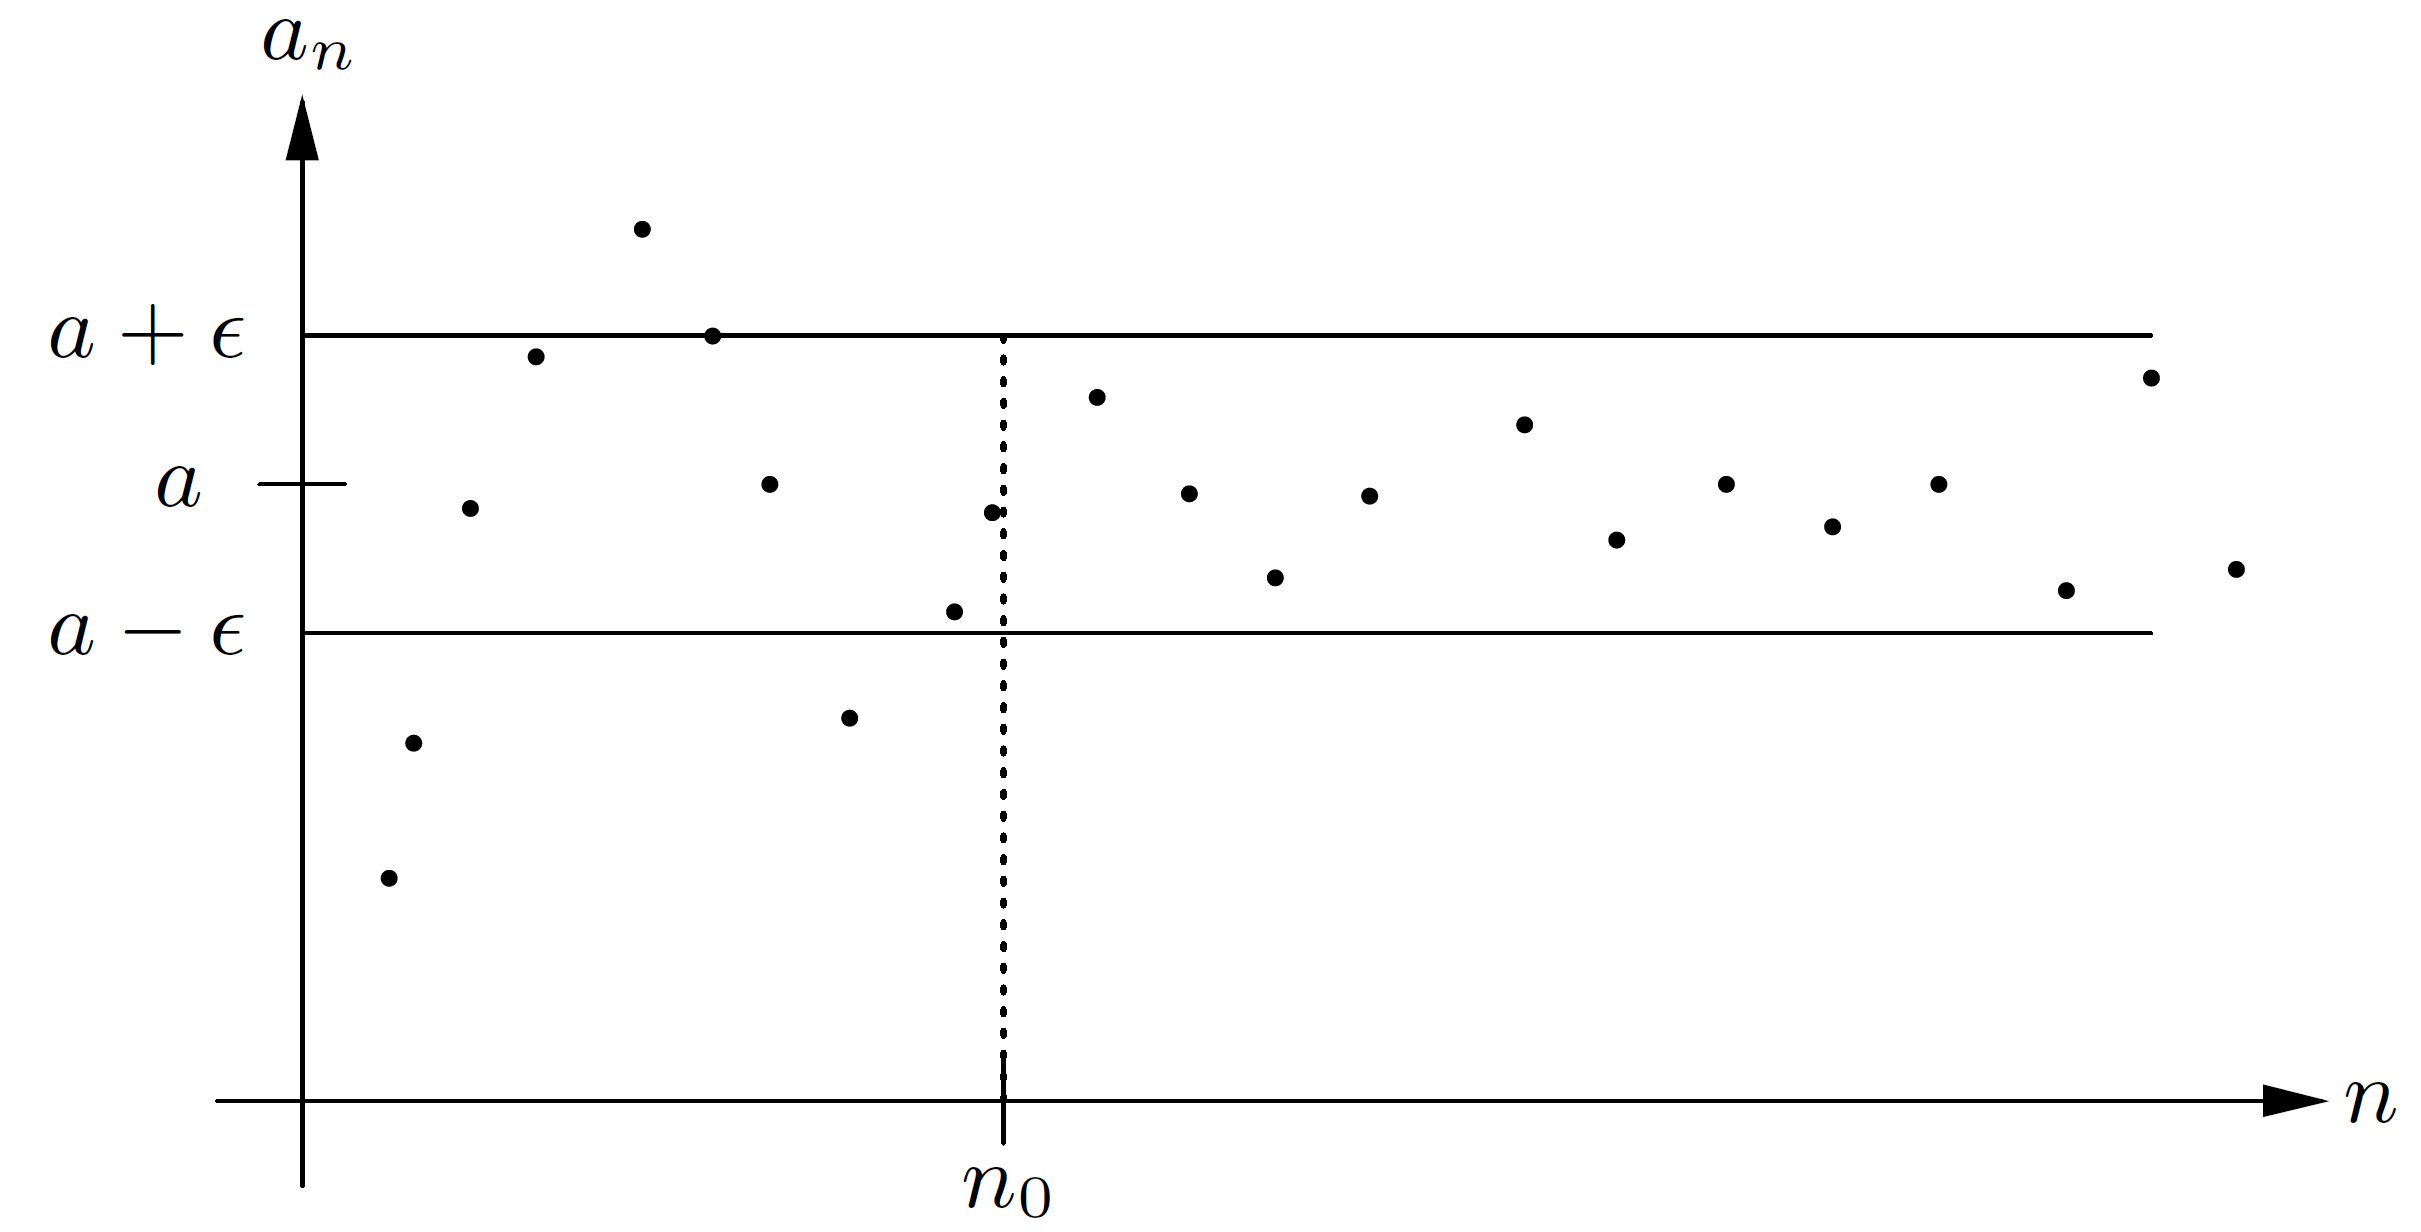
\includegraphics[width=0.95\linewidth]{img/konvergenz.png}
%\end{figure}
\end{warmup}

\begin{warmup}
\Bem Einfach ausgedrückt: Eine Folge $a_n$ konvergiert gegen $a\in \R$, falls
für jede beliebig klein gewählte Zahl $\epsilon > 0$ (z.B. $\epsilon =
10^{-10} \text{ oder }\epsilon = 0.00345$) eine von $\epsilon$ abhängige grosse
Zahl $N$ derart existiert, dass alle Folgeglieder $a_n$ mit $n\geq N$ in dem
Streifen $(a-\epsilon,a+\epsilon)$ liegen.

Da die Zahl $\epsilon$ beliebig klein gewählt werden kann, heisst dies, dass für
grosse $n$ die Folgenglieder $a_n$ beliebig nahe am Grenzwert $a$ liegen.
\end{warmup}

\Bem Man sagt, also dass der Grenzwert \emph{existiert}, falls der
Limes nicht $\pm \infty$ ist, und nicht $\pm c \neq
0$ ist. D.h. wenn der Grenzwert genau eine einzige Zahl
$a\in(-\infty,\infty)=\R$ ist, sagt man, dass er \emph{existiert}.

\sep

\Satz Grenzwerte sind eindeutig. Genauer: Ist $a_n$ sowohl gegen $a$ als auch
gegen $b$ konvergent, so gilt $a=b$.

\sep

\textbf{Beweis eines Grenzwertes mittels der Definition}

\Vorgehen Ungleichung mit Definition von und Grenzwert aufschreiben, $a_n$ und
$a$ einsetzen, nach $n$ (von $a_n$) auflösen, bzw. Ungleichung formulieren.

\begin{warmup}
\Bsp \ZZ $\lim_{n\to\infty}\frac{1}{n}=0$.
\[
\abs{a_n - a}= \abs{\tfrac{1}{n} - 0} = \abs{\tfrac{1}{n}} \stackrel{!}{<}
\epsilon \Longrightarrow n > \tfrac{1}{\epsilon}
\]
Das heisst, um ein passendes $N\in \N$ zu finden, wählen wir einfach
\[
N := \ceil{\tfrac{1}{e}}
\]
Da $\tfrac{1}{\epsilon}$ nicht unbedingt in $\N$, sondern eher in $\R$ ist.

Für alle $n\geq N$ gilt somit $\abs{\frac{1}{n}-0}<\epsilon$. Das entspricht
genau der Definition von $\lim_{n\to\infty} \frac{1}{n}=0$.

\Bsp \ZZ $\lim_{n\to\infty} \frac{3n^2+4}{2n^2+1}=\frac{3}{2}$.
\[
\abs{a_n - a} = \abs{\tfrac{3n^2+4}{2n^2+1}-\tfrac{3}{2}}
= \abs{\tfrac{6n^2+8-6n^2-3}{4n^2+2}} 
= \tfrac{5}{4n^2+2} \stackrel{!}{<} \epsilon
\]
\[
\Longrightarrow 4n^2+2 > \tfrac{5}{\epsilon} \Longrightarrow n >
\sqrt{\tfrac{5}{4\epsilon}-\tfrac{1}{2}}.
\]
Das heisst wir wählen
\[
N:= \ceil{\sqrt{\tfrac{5}{4\epsilon}-\tfrac{1}{2}}} \quad \text{dann gilt:}
\quad
\forall n\geq N : \abs{\tfrac{3n^2+4}{2n^2+1}-\tfrac{3}{2}} < \epsilon.
\]
Das entspricht genau der Definition von $\lim_{n\to\infty}
\frac{3n^2+4}{2n^2+1}=\frac{3}{2}$.
\end{warmup}

\Bsp \ZZ $\lim_{n\to\infty} n^{\frac{1}{n}} = 1$.
\[
\abs{a_n - a}=\abs{n^{\frac{1}{n}}-1} \stackrel{!}{<} \epsilon
\Longrightarrow
n < (\epsilon + 1)^n.
\]
\Trick Die letzte Ungleichung ist nicht einfach zu lösen, aber es gibt einen
Trick dafür: Wir formen sie in eine stärkere aber einfachere Ungleichung um,
anhand des binomischen Lehrsatzes, meistens genügt es dafür das zweite oder
dritte Glied zu nehmen:
\[
(1+\epsilon)^n = \underbrace{1 + n\epsilon}_{\geq 0} + \tfrac{n(n-1)}{2}\epsilon
^2
\underbrace{+ \ldots + \epsilon ^n}_{\geq 0}
\geq 
\tfrac{n(n-1)}{2}\epsilon^2
\]
Die Idee ist jetzt, die Ungleichung $n<(\epsilon + 1)^n$ durch 
\[
n < \tfrac{n(n-1)}{2}\epsilon^2
\]
zu ersetzen. Die neue Ungleichung ist stärker, da jede Lösung der zweiten
Ungleichung  auch eine Lösung der ersten Ungleichung ist.
\[
n < \tfrac{n(n-1)}{2}\epsilon^2
\Longrightarrow 
1 < \tfrac{(n-1)}{2}\epsilon^2
\Longrightarrow 
\tfrac{2}{\epsilon^2}+1 < n
\]
Das heisst für ein gegebenes $\epsilon$, wenn wir $N$ so wählen:
\[
N:= \ceil{\tfrac{2}{\epsilon^2}+1}
\quad \text{ dann gilt } \quad 
\forall n \geq N : \abs{n^{\frac{1}{n}}-1} < \epsilon
\]
Das heisst, alle Folgeglieder sind beliebig nahe an $1$, was der Definition 
$\lim_{n\to\infty} n^{\frac{1}{n}} = 1$ entspricht.

\sep

\subsubsection{5.2.2 Divergenz}

\Def Eine Folge $a_n$ ist \emph{divergent}, falls
\[
\forall K > 0 \ \exists N=N(K)\in\N, \text{ s.d. } \forall n\geq N \colon
\abs{a_n} > K.
\]
\begin{warmup}
Notiert wird
\[
\lim_{n\to\infty} a_n = \infty.
\]

\todo{Wirklich $+\infty$ ?}

\todo: Bild
\end{warmup}

\Bem Einfach ausgedrückt: Eine Folge $a_n$ divergiert, falls für jede beliebig
gross gewählte Zahl $K>0$ eine von $K$ abhängige grosse Zahl $N$ existiert, derart
dass alle Folgenglieder $a_n$ mit $n \geq N$ im Betrag grösser als $K$ sind.

\Wichtig Da die Zahl $K$ beliebig gross gewählt werden kann, bedeutet dies, dass
für grosse $n$ die Folgenglieder $a_n$ beliebig gross sein können.

\sep

\Vorgehen[Bew. von Diverg. mittels Def.]

Wähle $K>0$ beliebig gross, finde ein $N\in\N$ sodass $\forall n\geq N$ gilt:
$n>\ldots K \ldots$. D.h. löse nach $n$ aus $a_n$ auf.

\begin{warmup}
\sep

\textbf{Beweis von Divergenz mittels der Definition}

\Bsp \ZZ $\lim_{n\to\infty} 3^{2n-1}= + \infty$.
Wir wählen eine beliebig grosse Zahl $K>0$. Dann müssen wir eine Zahl $N\in\N$
finden, derart dass $\forall n\geq N$ folgendes gilt
\[
\abs{a_n}=3^{2n-1} \stackrel{!}{>} K
\Longrightarrow
2n-1 > \log_3(K) = \tfrac{\log(K)}{\log(3)}
\]
\[
\Longrightarrow n > \tfrac{1}{2}\left(\tfrac{\log(K)}{\log(3)}+1\right)
\]
Es wird also $N:=\ceil{\tfrac{1}{2}\left(\tfrac{\log(K)}{\log(3)}+1\right)}$
gesetzt, sodass für alle $n\geq N$ folgendes gilt (nach Konstruktion)
\[
\abs{a_n} \geq K.
\]
Das entspricht genau der Def. von $\lim_{n\to\infty} 3^{2n-1}= + \infty$.

\sep
\end{warmup}

\subsection{5.3 Rechnen mit Grenzwerten}

\subsubsection{5.3.1 Rechenregeln}

Für die Bestimmung von Grenzwerten werden die folgenden Regeln benutzt:

\Satz Sind $a_n$ und $b_n$ konvergent mit Gernzwerten $a$ bzw. $b$, dann folgt
\begin{enumerate}
  \item $\begin{aligned}[t]\lim_{n\to\infty}(a_n+b_n) = a + b\end{aligned}$
  \item $\begin{aligned}\lim_{n\to\infty}a_n\cdot b_n = a \cdot b\end{aligned}$
  \item Falls $b_n,b\neq 0$, so gilt
  $\begin{aligned}\lim_{n\to\infty}\frac{a_n}{b_n}=\frac{a}{b}\end{aligned}$
  \item Falls $a_n\leq b_n \ \forall n \in \N$, so gilt $a\leq b$
\end{enumerate}

\sep

\begin{warmup}
\textbf{Beispiele und Tricks zum Rechnen mit Grenzwerten}

\Bsp In diesem Fall können wir die 3. Regel nicht wirklich anwenden, da
weder der Nenner noch der Zähler konvergieren. Eine einfache Umformung löst das
Problem:
\[
\lim_{n\to\infty} \frac{n}{n+1}
= \lim_{n\to\infty} \frac{n}{n(1+\frac{1}{n})}
= \lim_{n\to\infty} \frac{1}{1+\frac{1}{n}}
\stackrel{(3,1)}{=} = \tfrac{1}{1+0} = 1.
\]
\end{warmup}

\Trick Man schreibt also einen Faktor vor den nenner oder Zähler, den man gerne
kürzen möchte, streicht ihn dann heraus und fährt mit einem Term der sich für
die Regeln besser eignet weiter.

\begin{warmup}
\sep


\Bsp Hier kann man nicht gleich die 3. und 1. Regel anwenden, da man Summen und
Differenzen von $n$ hat, eine kleine Umformung hilft:
\[
a_n=\tfrac{n^2+4n-2}{2n^2-5n}
=\tfrac{n^2(1+\frac{4}{n}-\frac{2}{n^2})}{n^2(2 -\frac{5}{n})}
=\tfrac{1+\frac{4}{n}-\frac{2}{n^2}}{2 -\frac{5}{n}}
\to \tfrac{1}{2} \ (\text{für } n\to\infty)
\]
\end{warmup}

\Trick Das war eine Schreibweise, wie man sich den Limes sparen kann.

\Trick Grösste Potenz herausklammern, kürzen, so dass die Faktoren der
dominanten Potenzen übrig bleiben und ein Verhältnis erzeugen. Kann man auch im
Kopf machen.

\begin{warmup}
\sep

\Bsp 
\begin{align*}
a_n &= \sqrt{n}(\sqrt{n+2}-\sqrt{n})\\
&=\sqrt{n}(\sqrt{n+2}-\sqrt{n}) \cdot
\frac{\sqrt{n+2}+\sqrt{n}}{\sqrt{n+2}+\sqrt{n}}\\
&= \frac{\sqrt{n}((n+2)-n)}{\sqrt{n+2}+\sqrt{n}}
= \frac{2\sqrt{n}}{\sqrt{n+2}+\sqrt{n}}\\
&= \frac{2\sqrt{n}}{\sqrt{n}\sqrt{1+\frac{2}{n}}+\sqrt{n}}
= \frac{2}{\sqrt{1+\frac{2}{n}}+1} \to 1 \ (\text{für }
n\to\infty)
\end{align*}
\end{warmup}

\Trick Mit $1$ bzw. dem Konjugierten
des Nenners, Zählers oder Terms multiplizieren.

\Trick Wie vorher Faktor herausklammern, den man kürzen möchte.

\subsubsection{5.3.2 Das Sandwich Theorem}

\Satz (Sandwich Theorem) Es seien die drei Folgen $b_n \leq a_n \leq c_n$.
gegeben. Falls $b_n$ und $c_n$ konvergent sind mit $\lim_{n\to\infty} b_n =
\lim_{n\to\infty} c_n = L$, so ist auch $a_n$ konvergent und
\[
\lim_{n\to\infty} a_n = L.
\]

\begin{warmup}
\sep

\textbf{Grenzwerte bestimmen mit Sandwich Theorem}

\Bsp $a_n:= \frac{2n}{2^n}$

Für $n\geq 1$ gilt $2n \geq 1$, und für $n\geq 4$ gilt $2^n\geq n^2$. Deshalb
gilt:
\[
\frac{1}{2^n} \leq \frac{2n}{2^n} \leq \frac{2n}{n^2} = \frac{2}{n}  \
(\text{für }n\geq 4)
\]
Da die untere und obere Abschätzung beide gegen 0 konvergieren für $n\to\infty$,
konvergiert $a_n$ auch gegen 0.

\sep
\end{warmup}

\Trick Es reicht wenn die Abschätzung erst ab eine gewissen $n_0$ gilt.

\begin{warmup}
\sep
\end{warmup}

\Trick \begin{itemize}
  \item \textbf{Untere Abschätzung}: Zähler kleiner und/oder Nenner grösser
  \item \textbf{Obere Abschätzung}: Zähler grösser und/oder Nenner kleiner
\end{itemize}

\begin{warmup}
\sep

\Bsp $b_n:= \sqrt[n]{3^n+5^n}$
\[
\sqrt[n]{5^n} \leq \sqrt[n]{3^n+5^n} \leq \sqrt[n]{5^n+5^n} = 5\sqrt[n]{2} \leq
5 \sqrt[n]{n}
\]
Da die Äusseren Folgen nach 1 konvergieren konvergiert $b_n$ ebenfalls nach 1.

\sep
\end{warmup}

\subsection{5.4 Monotonie und Konvergenz}

\subsubsection{5.4.1 Monotonie und Beschränktheit}

\Def Eine Folge $a_n$ heisst
\begin{itemize}
  \item \emph{(streng) monoton wachsend}, falls \\ $a_n \ (<) \leq a_{n+1} \quad
  \forall n \text{ ab einem gewissen } n_0.$
  \item \emph{(streng) monoton fallend}, falls \\ $a_n \ (>) \geq a_{n+1} \quad
  \forall n \text{ ab einem gewissen } n_0.$
  \item \emph{nach oben bzw. nach unten beschränkt}, falls\\
  $\exists C \in \R, \text{ s.d. } \forall n \in \N \quad a_n \leq C \text{
  bzw. } a_n \geq C.$
\end{itemize}

\sep

\Trick Eine sehr einfache Methode, um die Monotonie zu zeigen, ist folgende. Man
ersetzt $n$ durch die kontinuierliche Variable $x$ und berechnet die Ableitung
nach $x$. Gilt $a'(x)\geq 0$ respektive $a'(x)\leq 0$, so ist die Folge monoton
wachsend respektive monoton fallend. (Nicht vergessen: $\forall n\in\N : n
\geq 0$).

\sep

\Satz Konvergente Folgen sind immer beschränkt:
\[
a_n \text{ konvergent} \Longrightarrow a_n \text{ beschränkt}.
\]
\Achtung
\[
a_n \text{ beschränkt} \not\Longrightarrow a_n \text{ konvergent}.
\]

\sep

\subsubsection{5.4.2 Monotone Konvergenz}

Falls zusätzlich Monotonie angenommen wird gilt auch quasi die Umkehrung des
vorangehenden Satzes.

\sep

\Satz \textbf{(Monotone Konvergenz)} Sei $a_n$ nach oben (bzw. nach unten)
beschränkt und monoton wachsend (bzw. fallend), dann ist $a_n$ konvergent.
\[
a_n \text{ na. o./u. besr. } \land \  a_n \text{ mon. wa./fa. }
\Longrightarrow a_n \text{ konv.}
\]

\Bem Dieser Satz ist besonders nützlich um die Konvergenz einer rekursiv
definierten Folge nachzuweisen.

\sep

\Vorgehen
\begin{enumerate}
  \item Berechne ein paar Terme von $a_n$ um ein Gefühl zu bekommen	
  \item Beweise mittels Induktion, dass die Folge monoton wachsend/fallend ist
  \item Beweise mittels Induktion, dass die Folge beschränkt ist, nimm dazu
  einen Grezwert, oder eine obere Schranke.
  \item Gelingen die beiden vorherigen Schritte, kann man daraus anhand des
  Satzes über Monotone Konvergenz folgern, dass $a_n\to a$ konvergiert. Um $a$
  zu bestimmen ersetzt man einfach $a_n$ bzw. $a_{n-1}$ in der
  Rekursionsgleichung durch $a$ und löst nach $a$ auf.
\end{enumerate}

\begin{warmup}
\sep

\textbf{Rekursiv definierte Folgen untersuchen mittels Monotoner Konvergenz:}

\Bsp Untersuche die rekursiv definierte Folge auf Konvergenz:
\[
a_1 = \sqrt{2} \qquad a_{n+1} =\sqrt{2 + a_n}
\]
Vorgehen
\begin{enumerate}
  \item Zuerst berechnen wir einige Terme um ein Gefühl für einen Möglichen
  Grenzwert zu bekommen. Wie wir sehen ist er wahrscheinlich 2.
  \item Dann beweisen wir, dass die Folge monoton wachsend ist mittels
  vollständiger Induktion 
  \[
  \forall n \in \N : a_n \leq a_{n+1}
  \]
  \item Dann beweisen, dass die Folge beschränkt ist mittels vollständiger
  Induktion. Als obere Schranke, dient der Grenzwert, den wir ermittelt haben.
  \[
  \forall n\in \N : a_n \leq 2
  \]
  \item Da $a_n$ beschränkt und monoton wachsend ist, muss $a_n$ gemäss dem
  Satz über Monotone konvergieren gegen einen Grenzwert $a$. Der Grenzwert kann
  ganz einfach bestimmt werden. Da $a_n$ und also auch $a_{n+1}$ gegen $a$ 
  konvergieren, können wir beide mit $a$ ersetzen 
  \[
  	a_{n+1} = \sqrt{2 + a_{n+1}} \Longrightarrow a = \sqrt{2+a}
  \]
  Wir bekommen somit eine Gleichung für den noch unbekannten Grenzwert $a$
  \[
  a = \sqrt{2+a} \Longrightarrow a^2 = 2 + a \Longrightarrow a^2-a-2=0
  \Longrightarrow a= 2.
  \]
\end{enumerate}

\sep

\Bsp Betrachte die rekursiv definierte Folge
\[
a_0 = 0, \quad a_{n+1} = \left(\frac{a_n}{2}\right)^2+1
\]
Zeige, dass die Folge $a_n$ monoton wachsend und nach oben beschränkt ist. Warum
folgt daraus die Konvergenz von $a_n$? Wie lautet der Grenzwert?

Wir berechnen zuerst einige Terme
\[
a_0 = 0, \quad a_1 = 1, \quad a_2 = \frac{5}{4}, \quad a_3 = \frac{89}{64},
\quad \ldots
\]
Die Zahlen suggerieren, dass die Folge monoton wachsend ist. Wir zeigen es per
Induktion, durchs ausrechnen haben wir die Verankerung schon gezeigt, hier noch
der Induktionsschritt. Anstatt $a_{n+1}\geq a_n$ zu zeigen, zeigen wir die dazu
äquivalente Aussage $a_{n+1}-a_n\geq 0$:
\[
a_{n+1} - a_n = \frac{a_n^2}{4} +1 -a_n = \frac{a_n^2-4a_n+4}{4} =
\frac{(a_n-2)^2}{4}\geq 0.
\]
Wir zeigen mittels vollständiger Induktion, dass $a_n\leq 2 \ \forall n\in\N$
gilt

Verankerung ($n=0$): $a_0 = 0 \leq 2$.

Induktionsschritt ($n\Longrightarrow n+1$): Wir nehmen an, dass
\[
a_n\leq 2
\]
gilt (Induktionsannahme). Es folgt
\[
a_{n+1}=\frac{a_n^2}{4}+1 \stackrel{a_n\leq 2}{\leq} \frac{2^2}{4} + 1 = 2.
\]
Nach dem Satz über monotone Konvergenz folgt, dass $a_n$ konvergiert. Was ist
der Grenzwert $a=\lim_{n\to\infty} a_n$? Da mit $a_n$ auch $a_{n+1}$ gegen $a$
konvergiert, gilt
\[
a_{n+1} =\left(\frac{a_n}{2}\right)^2 +
1
\Rightarrow a = \frac{a^2}{4} + 1
\Rightarrow \frac{(a-2)^2}{4} = 0
\Rightarrow a = 2.
\]

\sep
\end{warmup}

\Trick Sollte man eine Folge $a_n$ erhalten, die alternierend ist, dann kann man
den Grenzwert $a$ zuerst berechnen, und dann zeigen, dass die Absolutbeträge
folgender Folge
\[
b_n = a_n - a
\]
monoton fallend sind, d.h. $\abs{b_n}$ ist monoton fallend. Dann zeigt man, dass
$\abs{b_n}$ beschränkt ist. Somit konvergiert auch $b_n$ (ohne Betrag) und
ferner auch $a_n$.


\sep


\subsection{5.5 Teilfolgen}

\Def Sei $\Lambda \subset \N $ eine unendliche Teilmenge der natürlichen Zahlen
und $a_n$ eine Folge. Die Folgenglieder $a_n$ mit $n\in \Lambda$ bilden eine
\emph{Teilfolge} $\{a_n\}_{n\in\Lambda}$.

\Achtung $\Lambda$ muss unendlich viele Elemente enthalten!

\Achtung $\Lambda$ muss streng monoton wachsend sein.

\sep

\subsubsection{5.5.1 Der Satz von Bolzano-Weierstrass}

\Satz \textbf{(Bolzano-Weierstrass)} Jede bschränkte Folge in $\R$ besitzt eine
konvergente Teilfolge.
\[
a_n \text{ beschr. } \Longrightarrow \exists \Lambda \subset \N \text{ s.d.
}\{a_n\}_{n\in\Lambda} \text{ konv.}
\]

\sep

\subsection{5.6 Limes superior und Limes inferior}

\Def Sei $a_n$ eine beschränkte und nicht notwendigerweise konvergente Folge.
Für alle $n\in\N$ definiere
\[
b_n :=\sup \{a_k\setsep k\geq n\} = \sup\{a_n,a_n+1, \cdots\}.
\]
Explizit:
\begin{align*}
b_0 &= \sup\{a_0,a_1,a_2,\ldots\}\\
b_1 &= \sup\{a_1,a_2,a_3,\ldots\}\\
b_2 &= \sup\{a_2,a_3,a_4,\ldots\}\\
&\ \vdots
\end{align*}
Das heisst $b_n$ ist eine Teilfolge von $a_n$. Wir fragen uns. Ist $b_n$
konvergent? Die Folge $b_n$ ist monoton fallend, d.h.
\[
b_n \geq b_{n+1},
\]
weil für die Bestimmung von $b_{n+1}$ das Supremum über eine kleinere Anzahl von
Folgegliedern von $a_n$ genommen wird als für $b_n$. Die Folge $b_n$ ist auch
beschränkt, weil $a_n$ beschränkt ist. Der Satz über monotone Konvergenz
impliziert somit, dass $b_n$ konvergiert. Der Limes von $b_n$ wird \emph{Limes
superior} von $a_n$ genannt. Notiert wird
\[
\lim_{n\to\infty} b_n = b =: \limsup_{n\to\infty} a_n.
\]
Analog kann man für alle $n\in\N$ die Folge
\[
c_n:=\inf\{a_k\setsep k\geq n\} = \inf\{a_n, a_{n+1}, \ldots\}
\]
betrachten. Die so definierte Teilfolge $c_n$ ist monoton wachsend, weil für die
Bestimmung von $c_{n+1}$ das Infimum über eine kleinere Anzahl von
Folgengliedern von $a_n$ bestimmt wird, als für $c_n$. Sie ist auch beschränkt,
da $a_n$ beschränkt ist, und folglich konvergent. Der Limes von $c_n$ heisst
\emph{Limes inferior} von $a_n$. Notiert wird
\[
\lim_{n\to\infty}c_n= c =:\liminf_{n\to\infty} a_n.
\]
\Bem Falls die Folge nach unten oder nach oben unbeschränkt ist, setzt man
\[
\limsup_{n\to\infty} a_n = +\infty \quad \text{bzw.}\quad
\liminf_{n\to\infty} a_n = -\infty.
\]
\Bem Falls die Folge selbst konvergent ist, stimmen $\limsup_{n\to\infty} a_n$
und $\liminf_{n\to\infty} a_n$ überein und sind gleich $\lim_{n\to\infty} a_n$.

\sep

\Satz Es gilt
\[
\lim_{n\to\infty} a_n = a \Longleftrightarrow \limsup_{n\to\infty} a_n =
\liminf_{n\to\infty} a_n = \lim_{n\to\infty} a_n
\]

\Bem In anderen Worten: Für konvergente Folgen ist die Betrachtung mit $\limsup$
und $\liminf$ unnötig, da es keinen Unterschied zwischen $\limsup$. $\liminf$
und dem üblichen Limes gibt. Dieser Unterschied wird relevant, sobald $a_n$
selbst nicht konvergiert, wie dies zum Beispiel bei stückweise definierten
Folgen der Fall ist.

\sep

\Bsp
\[
\limsup_{n\to\infty} n \sin^2\left(\frac{n\pi}{2}\right) = +\infty
\quad
\liminf_{n\to\infty} n \sin^2\left(\frac{n\pi}{2}\right) = 0
\]
\Bsp
\begin{align*}
\limsup_{n\to\infty} \sqrt[n]{\abs{5^n+(-5)^n}} &\stackrel{n \text{
gerade}}{=} \limsup_{n\to\infty} 
\sqrt[n]{2\cdot 5^n}\\ &= \limsup_{n\to\infty}  5 \sqrt[n]{2} = 5.
\end{align*}

\sep

\subsection{5.7 Cauchy Folgen}

\Def Eine Folge $a_n$ heisst \emph{Cauchy Folge} falls
\[
\forall\epsilon > 0 \ \exists N = N(\epsilon)\ \forall n,m\geq N : \ 
\abs{a_n-a_m}\leq \epsilon.
\]
Anschaulich gesprochen ist eine Folge genau dann eine Cauchy-Folge, wenn ihre
Folgenglieder für wachsende Indizes immer enger zusammenrücken.

\sep 

\Satz (Cauchy-Kriterium) Sei $a_n$ eine reelle (oder komplexe) Folge. Dann gilt:
\[
a_n \text{ konvergiert} \Longleftrightarrow a_n \text{ ist eine Cauchy-Folge}.
\]

\Bem Konvergente Folgen sind immer Cauchy-Folgen. Denn bei einer konvergenten
Folge kommen die Folgenglieder $a_n$ nicht nur dem Grenzwert $a$ beliebig nahe,
sondern die Folgenglieder kommen sich auch untereinander ab einem gewissen Index
beliebig nahe.

Umgekehrt, sind auch reelle (oder
komplexe) Cauchy Folgen konvergent. Es gibt aber Situationen (z.B bei
rationalen Folgen) wo dies nicht der Fall ist.

Wenn man zum Beispiel, eine Folge in $\Q$ betrachtet, die in $\R$ nach
$\sqrt{2}$ konvergieren würde, in $\Q$ ist sie sehrwohl Cauchy-konvergent, aber
sie ist in $\Q$ nicht konvergent, da $\sqrt{2}\not\in\Q$ und der Grenzwert somit
nicht existiert.
\[
\text{Konvergente Folgen } \subseteq \text{ Cauchy Folgen}
\]
\Beweis Au der Definition von der Konvergenz existiert also der GW
$a=\lim_{n\to\infty} a_n$, somit gilt für alle $n,m\geq N$:
\begin{align*}
\abs{a_m-a_n} &= \abs{a_m - a + a - a_n}
\\ &\leq
\underbrace{\abs{a_m-a}}_{<\epsilon}
+\underbrace{\abs{a-a_n}}_{<\epsilon} < 2\epsilon.
\end{align*}
Somit ist jede konvergente Folge $a_n$ eine Cauchy Folge.


\sep

\Def Metrische Räume, welche die Eigenschaft haben, dass jede Cauchy-Folge
konvergiert, werden \emph{(metrisch) vollständige Räume} genannt.

\Bsp $\N$, $\R$ und $\C$ sind vollständige Räume. $\Q$ hingegen nicht.

\Bem In $\N$ sind die Cauchy Folgen, falls $\epsilon < 1$ gewählt wirt einfach
ab $N(\epsilon)$ konstant. Somit ist $\N$ auch ein vollstänidger Raum.

\sep

\textbf{Beweise von Konvergenz/Divergenz anhand des Cauchy Kriteriums}

Cauchy-Folgen liefern im Prinzip ein handliches Kriterium für die Konvergenz
einer Folge in $\R$, denn es genügt zu zeigen, dass eine vorgelegte Folge eine
oder keine Cauchy-Folge ist, um Konvergenz oder Divergenz nachzuweisen, ohne den
Grenzwert bereits zu kennen zu müssen. Dieses Kriterium ist jedoch nur selten
geeignet, da wir den Grenzwert der zu untersuchenden Folge durch dieses
Verfahren nicht ermitteln können.

\Trick Bei beweisen über die Definition von Cauchy-Konvergenz ist es immer eine
gute Idee, o.B.d.A. $m\geq n$ (oder $n\geq m$) zu fixieren.

\sep

\Vorgehen $\epsilon$ fixieren, o.B.d.A. sei $m\geq n$, Terme zusammennehmen,
nach oben abschätzen, $m$ rauskürzen, Formel für $n$ in Abhängigkeit von
$\epsilon$ ermitteln.


\begin{warmup}
\sep

\Vorgehen Widerspruchsbeweis \todo

\sep

\Bsp Ist die Folge $a_n=\frac{n-1}{2n}$ konvergent?
Wir überprüfen, ob $\frac{n-1}{2n}$ eine Cauchy-Folge ist. Dazu wählen wir ein
(beliebig kleines) $\epsilon$. Nun, sei o.B.d.A. $m\geq n$:
\begin{align*}
\abs{a_n - a_m} &= \abs{\frac{n-1}{2n}-\frac{m-1}{2m}}
= \abs{\frac{m(n-1) -n(m-1)}{2mn}}\\
&= \abs{\frac{mn - m -mn +n}{2mn}} = \abs{\frac{n-m}{2mn}}\\
&\stackrel{m\geq n}{=} \frac{m-n}{2mn} \leq \frac{m}{2mn}=\frac{1}{2n}
\stackrel{!}{<}\epsilon 
\end{align*}
\[
\Longrightarrow N:=\ceil{\frac{1}{\epsilon}}.
\]
Da ein solches $N(\epsilon)$ gefunden werden kann, ist die folge
Cauchy-konvergent. Da alle Cauchy-Folgen in $\R$ konvergieren ist $a_n$ somit
konvergent.

\sep

\Bsp (Nicht (Cauchy) konvergent, harmonische Reihe) Ist die harmonische Reihe
\[
\sum_{k=1}^\infty \frac{1}{k} = \lim_{n\to\infty} \sum_{k=1}^n\frac{1}{k}
\]
konvergent? (Hinweis: betrachte die Folge $a_n = \sum_{k=1}^n\frac{1}{k}$ und
überlege, ob $a_n$ eine Cauchy-Folge ist.)

Die harmonische Reihe ist als Grenzwert der Folge $a_n$ definiert. Wir
überprüfen, üb $a_n$ eine Cauchy-Folge ist. Wir betrachten dazu
\[
a_{2n} - a_n = \frac{1}{2n} + \underbrace{\frac{1}{2n-1}}_{\leq \frac{1}{2n}} +
\ldots +
\underbrace{\frac{1}{n+1}}_{\leq \frac{1}{2n}} \geq n\cdot\frac{1}{2n} =
\frac{1}{2}.
\]
Die Folge $a_n$ kann daher keine Cauchy-Folge sein, sie ist also divergent.

\sep

\Bsp ((Cauchy) konvergent, alternierende harmonische Reihe)
Ist die folgende Reihe
\[
\sum_{k=1}^{\infty} \frac{(-1)^k}{k}
= \lim_{n\to\infty} \sum_{k=1}^{n} \frac{(-1)^k}{k}
\]
konvergent? (Hinweis: betrachte die Folge $a_n=\sum_{k=1}^{n} \frac{(-1)^k}{k}$
und überlege, ob $a_n$ eine Cauchy-Folge ist.)

Sei $\epsilon > 0$, und o.B.d.A $m\geq n$, dann suchen wir ein $N(\epsilon)$, so
dass gilt
\begin{align*}
\abs{a_m - a_n}
&= \abs{ \sum_{k=1}^{m} \frac{(-1)^k}{k} - 
 \sum_{k=1}^{n} \frac{(-1)^k}{k}}
 \stackrel{m>n}{=} \abs{ \sum_{k=n+1}^{m} \frac{(-1)^k}{k} }\\
&= \abs{ \frac{(-1)^{n+1}}{n+1} + \frac{(-1)^{n+2}}{n+2} + \cdots
\frac{(-1)^{m}}{m}}\\
&= \abs{(-1)^{n+1}\left(\frac{1}{n+1}-\frac{1}{n+2}+\cdots
+\frac{(-1)^{n+m+1}}{m}\right)}\\
&= \abs{\frac{1}{n+1}-\frac{1}{n+2}+\cdots
+\frac{(-1)^{n+m+1}}{m}}\\
\end{align*}
Wir untersuchen nun die Terme ab $n+2$
\[
\abs{\frac{1}{n+1}-\left(\underbrace{\frac{1}{n+2}-\frac{1}{n+3}}_{\geq
0}+\cdots +\frac{(-1)^{n+m+1}}{m}\right)}\\
\]
Das Argument mit $\geq 0$ kann für alle aufeinanderfolgenden Termen fortgeführt
werden. Falls $m+n$ gerade ist geht es in Zweierpäärchen auf, falls $m+n$
ungerade ist bleibt $1/m$ alleine übrig, und das ist auch $\geq 0$.

Daraus folgt, dass der Term folgendermassen abgeschätzt werden kann.
\begin{align*}
\abs{a_m - a_n}
&= \abs{\frac{1}{n+1}-\frac{1}{n+2}+\cdots+\frac{(-1)^{n+m+1}}{m}}\\
&\leq \frac{1}{n+1} \stackrel{!}{<} \epsilon \Longrightarrow N :=
\ceil{\frac{1}{\epsilon}-1}.
\end{align*}

Somit ist die alternierende Reihe konvergent, da für jedes $\epsilon>0$ ein
$N(\epsilon)$ gefunden werden, kann so dass alle Folgenglieder ab $N(\epsilon)$
einen kleineren Abstand zueinander als $\epsilon$ haben.

\sep
\end{warmup}


\newpage

\section{6. Grenzwerte von Funktionen}

Bisher haben wir nur Grenzwerte von Folgen $a_n$ für $n\to\infty$ betrachtet.
Jetzt wollen wir auch beliebige Funktionsausdrücke $f(x)$ mit $x\in\R$
betrachten und deren Verhalten für $x\to a$ untersuchen.

\subsection{6.1 Der Grenzwert einer Funktion}

\Def Sei $f$ eine Funktion, welche auf einem offenen Intervall $I\subset \R	$
definiert ist, das den Punkt $a$ enthält. Man sagt $f$ besitzt an der Stelle $a$
den Grenzwert $L\in \R$, geschrieben
\[
\lim_{x\to a} f(x) = L,
\]
falls
\[
\forall \epsilon > 0 \ \exists \delta > 0 \ \forall x, \ 
\abs{x-a}<\delta \colon \abs{f(x)-L}<\epsilon.
\]

\begin{warmup}
\todo{Bild aktivieren}
%\begin{figure}[H]
	%\centering
  	%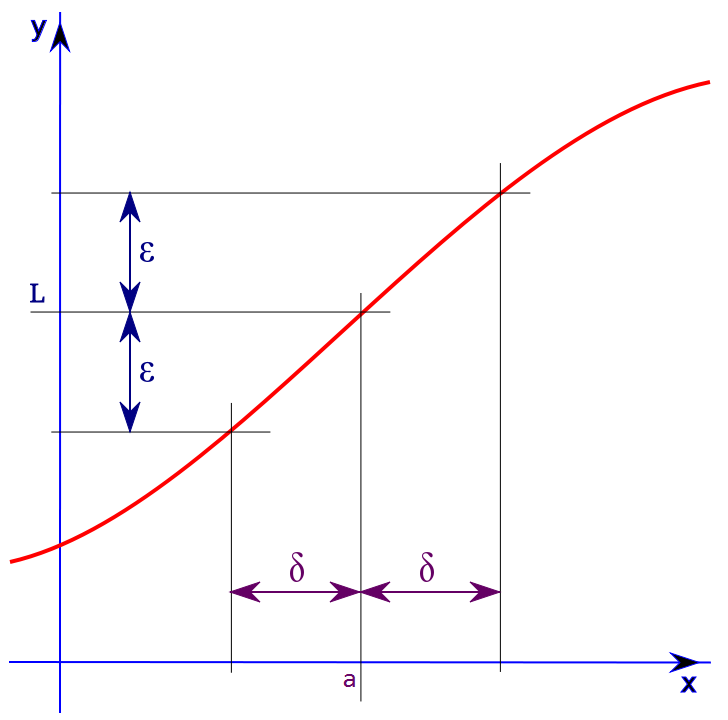
\includegraphics[width=0.5\linewidth]{img/epsilon-delta.png}
%\end{figure}
\end{warmup}

\Bem In Worten: $\lim_{x\to a} f(x)=L$ bedeutet, dass für jede beliebig klein
gewählte Zahl $\epsilon > 0$ eine Zahl $\delta > 0$ existiert, welche i. Allg.
von $\epsilon$ abhängt, sodass für alle $x$ in $(a - \delta, a + \delta)$ gilt
$f(x)\in (L-\epsilon, L+\epsilon)$.

\sep

Es ist of nützlich, links- und rechtsseitige Grenzwerte zu definieren.

\Def $f\colon I\subset \R \to \R$ hat an der Stelle $a\in I$ den
\emph{linksseitigen Grenzwert} $L\in\R$, geschrieben
\[
\lim_{x\to a^-} f(x) = L,
\]
falls
\[
\forall\epsilon > 0 \ \exists \delta >0, \text{ s.d. } \forall x\in(a-\delta,a)
\colon \abs{f(x)-L}<\epsilon.
\]
Analog hat $f$ an der Stelle $a$ den \emph{rechtsseitigen Grenzwert} $L\in\R$,
geschrieben
\[
\lim_{x\to a^+} f(x) = L,
\]
falls
\[
\forall\epsilon > 0 \ \exists \delta >0, \text{ s.d. } \forall
x\in(a,a+\delta) \colon \abs{f(x)-L}<\epsilon.
\]

\sep

\Satz Sei $f\colon I\subset\R\to\R$ und $a\in I$. Die folgenden Aussagen sind
äquivalent:
\begin{enumerate}[label=\roman*)]
  \item $f$ besitzt in $a$ den Grenzwert $L$;
  \item $f$ besitzt an der Stelle $a$ einen linksseitigen und einen
  rechtsseitigen Grenzwert und für diese gilt
  \[
  \lim_{x\to a^-} f(x) = \lim_{x\to a^+} f(x) = L.
  \]
\end{enumerate}

\sep

Auch in den Fällen, wo der Grenzwert an der Stelle $a$ unendlich ist, kann man
analoge Definitionen aufstellen.

-

\Def $\lim_{x\to a} f(x)= + \infty$ bedeutet, dass
\[
\forall M>0 \ \exists\delta > 0, \text{ s.d. } \forall x, \ \abs{x-a}<\delta
\text{ gilt } f(x) > M. 
\]
D.h. egal wie gross wir $M$ wählen, wir finden immer noch ein $\delta$, so dass
für alle $x$ in dieser Umgebung $f(x)$ grösser als $M$ ist.

-

\Def $\lim_{x\to a} f(x)= - \infty$ bedeutet, dass
\[
\forall M<0 \ \exists\delta > 0, \text{ s.d. } \forall x, \ \abs{x-a}<\delta
\text{ gilt } f(x) < M. 
\]
Analog: Egal wie gross wir eine negative Zal $M$ wählen\ldots

-

\Def $\lim_{x\to a} f(x)= \infty$ bedeutet, dass
\[
\forall M>0 \ \exists\delta > 0, \text{ s.d. } \forall x, \ \abs{x-a}<\delta
\colon \abs{f(x)} > M. 
\]
\Bsp $a_n:=\frac{1}{x}$ konvergiert von rechts gegen $+\infty$ und von links
gegen $-\infty$. Es ist also einfach eine Zusammensetzung der oberen beiden
Definitionen.

-

\Def $\lim_{x\to \infty} f(x)= \infty$ bedeutet, dass
\[
\forall M>0 \ \exists N > 0, \text{ s.d.} \forall x, \ \abs{x}>N
\text{ gilt } \abs{f(x)} > M. 
\]
D.h. egal wie gross wir $M$ wählen, wir finden immer ein $N$, so dass alle $x$,
$\abs{x}\geq N$ der Funktionswert $f(x)$ im Betrag grösser ist als $M$.

\sep

\Vorgehen[Ber. v. GW mittels $\epsilon$-$\delta$-Def.]

\ZZ $f(x)\to a$ für $x\to x_0$. \Beweis Fixiere $\epsilon >0$ als beliebig
klein, dann zeige, dass es ein $\delta > 0$, sodass für alle
$x\in(x-\delta,x+\delta)$ gilt:
$\abs{f(x)-a}<\epsilon$. Dazu schreibt man die Gleichung $\abs{f(x)-a}<\epsilon$
auf, oft läuft es aufs Aufklappen des Betrags hinaus.
Bringe dann $x$ in die Mitte der Ungleichungen, links und rechts sollte ein Term
in Abhängigkeit von $\epsilon$ stehen. Die beiden Therme bilden die
$\delta$-Umgebung von $x$ für ein $\epsilon$, diese kann man Gleichsetzen mit
$(a-\delta_1, a+\delta_2)$ , dadurch bestimmt man dann $\delta_1$ und
$\delta_2$. Schlussendlich ergibt sich, dass für $\delta:=\min{\delta_1,
\delta_2}$ die obige ungleichung erfüllt ist.

\begin{warmup}
\sep

\textbf{Berechnung von Grenzwerten mittels der $\epsilon-\delta$-Definition}

\Bsp \ZZ $\lim_{x\to 5} \frac{x-5}{\sqrt{x}-\sqrt{5}}=2\sqrt{5}$

Dazu wählen wir ein beliebig kleines $\epsilon > 0$ aus. Wir müssen zeigen, dass
es ein $\delta<0$ gibt, sodass für alle $x\in(5-\delta,5+\delta)$ Folgendes gilt
\[
\abs{\frac{x-5}{\sqrt{x}-\sqrt{5}}-2\sqrt{5}} \stackrel{!}{<} \epsilon.
\]
Eine kleine Umformung (Trick mit Konjugiertem, resp. 1 multiplizieren) liefert
\[
\abs{\frac{x-5}{\sqrt{x}-\sqrt{5}}-2\sqrt{5}} = \abs{\sqrt{x}-\sqrt{5}}
\stackrel{!}{<} \epsilon
\Longrightarrow
-\epsilon< \sqrt{x} - \sqrt{5} < \epsilon
\]
\Trick Bei der letzten Implikation haben wir den Betrag aufgeklappt.

Nun können wir weiterfahren
\begin{align*}
&-\epsilon < \sqrt{x} - \sqrt{5} < \epsilon\\
\Longleftrightarrow \quad
&\sqrt{5}-\epsilon < \sqrt{x} < \sqrt{5} + \epsilon\\
\Longleftrightarrow \quad
&(\sqrt{5}-\epsilon)^2 < x < (\sqrt{5} + \epsilon)^2
\end{align*}

Das bedeutet, dass für alle $x$, die die obige Ungleichung erfüllen
$\abs{f(x)-2\sqrt{5}}<\epsilon $ gilt.

Da $\epsilon$ eine sehr kleine Zahl ist, liegen die Werte
$(\sqrt{5}-\epsilon)^2$ und $(\sqrt{5} + \epsilon)^2$ sehr nahe an 5, also
definiert $((\sqrt{5}-\epsilon)^2,(\sqrt{5} + \epsilon)^2)$ eine
$\delta$-Umgebung von $5$. Das Intervall $((\sqrt{5}-\epsilon)^2,(\sqrt{5} +
\epsilon)^2)$ schreiben wir als
\[
(5-\delta_1,5+\delta_2),
\]
mit $\delta_1= 5-(\sqrt{5}-\epsilon)^2$ und $\delta_2= (\sqrt{5}+\epsilon)^2-5$.
Das Intervall ist asymmetrisch.  Wir setzen somit $\delta =
\min\{\delta_1,\delta_2\}$, damit wir mit Sicherheit
$\abs{f(x)-2\sqrt{5}}<\epsilon$ erfüllen. Für die so gewählte Zahl $\delta$ gilt
also
\[
\abs{x-5}<\delta \Longrightarrow \abs{f(x)-2\sqrt{5}}<\epsilon.
\]
Das ist genau die Definition von $\lim_{x\to 5}
\frac{x-5}{\sqrt{x}-\sqrt{5}}=2\sqrt{5}$.

-

\Bsp \ZZ $\lim_{x\to 0}\frac{1}{x^2}=+\infty$

Wir wählen ein beliebig grosses $M>0$. Wir müssen überprüfen, ob ein $\delta>0$
existiert, sodass für alle $\abs{x-0}<\delta$ folgendes gilt
\[
\frac{1}{x^2}\stackrel{!}{>}M.
\]
Das impliziert
\[
\frac{1}{x^2}\stackrel > M \Longrightarrow
x^2 > \frac{1}{M} \Longrightarrow
\abs{x}<\frac{1}{\sqrt{M}}.
\]
Dies bedeutet, dass für alle $x$ mit $\abs{x}<\frac{1}{\sqrt{M}}$ das folgende
gilt $1/x^2 > M$. Wir setzen also $\delta = 1/\sqrt{M}$. Für die so gewählte
Zahl $\delta$ gilt
\[
\abs{x-0}<\delta \Longrightarrow \frac{1}{x^2} > M.
\]
Das entspricht genau der Definition von $\lim_{x\to 0}\frac{1}{x^2}=+\infty$.


\sep

\end{warmup}



\newpage

\section{7. Rechnen mit Grenzwerten}

In diesem Kapitel studieren wir nützliche Techniken, um Grenzwerte von
Funktionen effizient berechnen zu können.

\subsection{7.1 Prinzip}

\Satz Falls die Grenzwerte
\[
\lim_{x\to a} f(x) \quad \text{und} \quad \lim_{x\to a} g(x)
\]
existieren, so werden die Grenzwerte mittels der folgenden Rechenregeln
ermittelt

\begin{enumerate}[label=\arabic*)]
  \itemsep5px 
  \item $\begin{aligned}[t]
  \lim_{x\to a} \left(f(x) \pm g(x)\right)
  =
  \lim_{x\to a} f(x) \pm \lim_{x\to a} g(x)
  \end{aligned}$
  \item $\begin{aligned}[t]
  \lim_{x\to a} \left(c\cdot f(x)\right)
  = c\cdot \lim_{x\to a} f(x)
  \end{aligned}$
  \item $\begin{aligned}[t]
  \lim_{x\to a} \left(f(x) \cdot g(x)\right)
  =
  \lim_{x\to a} f(x) \cdot \lim_{x\to a} g(x)
  \end{aligned}$
  \item $\begin{aligned}[t]
  \lim_{x\to a} \frac{f(x)}{g(x)}
  =
  \frac{\lim_{x\to a} f(x)}{\lim_{x\to a} g(x)}, \quad \text{falls }\lim_{x\to
  a} g(x)\neq 0
  \end{aligned}$
  \item $\begin{aligned}[t]
  \lim_{x\to a} f(x)^{g(x)}
  =
  \left(\lim_{x\to a} f(x)\right)^{\lim_{x\to a} g(x)}
  \end{aligned}$
\end{enumerate}

\sep

\subsection{7.2 (Un)-entscheidbare Situationen}

Die Rechenregeln, die wir im vorigen Abschnitt kennengelernt haben, gelten nur,
falls die Grenzwerte $\lim_{x\to a} f(x)$ und $\lim_{x\to a} g(x)$ beide
existieren.

In speziellen Situationen darf man sie trotzdem verwenden, auch wenn einer oder
beide Grenzwerte nicht existieren. Man notiert oft

\textbf{Entscheidbare Fälle}
\[
\frac{1}{0} = \infty,
\quad
\frac{1}{\infty} = 0,
\quad
\infty + \infty = \infty,
\]
\[
0 + \infty = \infty,
\quad
0^\infty = 0,
\quad
\infty^\infty = \infty.
\]
Die folgenden Fälle nennen wir \emph{unentscheidbar}. Hier ist das Resultat als
nicht a-priori entscheidbar.

\textbf{Unentscheidbare Fälle}
\[
\frac{0}{0}, \quad \frac{\infty}{\infty}, \quad \infty-\infty, \quad
1^{\infty}, \quad \infty^{0}, \quad 0^0, \quad 0\cdot\infty.
\]
Diese Fälle brauchen eine spezielle Betrachtung. Die verschiedenen Tricks,
welche wir in den folgenen Abschnitten kennenlernen werden, dienen dazu, diese
problematischen Fälle zu untersuchen.

\begin{warmup}
\subsection{Overview of Limit Tricks}

Bei unetscheidbaren Situationen können folgende Tricks helfen:

\begin{itemize}
  \item Binomische Formeln rückwärts anwenden, d.h. faktorisieren und kürzen.
  \item Grösste Potenz in Brüchen Faktorisieren und kürzen.
  \item Bekannte Limites verwenden (Aufteilen in Faktoren)
  \item Trigonometrische Identitäten
  \item Logarithmische Identitäten
  \item Dominante Terme erkennen
  \item Mit Sandwich Theorem nach unten und oben abschätzen. Dann aufgrund von
  Gleichheit und Eindeutigkeit argumentieren.
  \item \todo Zusammenfassende Liste
\end{itemize}
\end{warmup}

\subsection{7.3 Das Sandwich Theorem}

\Satz Aus $g(x)\leq f(x)\leq h(x)$ für $x$ in der Nähe von $a$ und
\[
\lim_{x\to a} g(x) = \lim_{x\to a} h(x) = L
\]
folgt
\[
\lim_{x\to a} f(x) = L.
\]

\sep

\Bsp Zu bestimmen sei $\lim_{x\to 0}\sqrt{x}e^{\sin(\frac{\pi}{x})}$.

Wir schätzen dazu nach unten und oben ab
\[
0\leftarrow \sqrt{x}e^{-1} \leq \sqrt{x}e^{\sin(\frac{\pi}{x})} \leq
\sqrt{x}e^{1}\rightarrow 0 \ \ \ (\text{für }x\to \infty)
\]
Es folgt, dass der Grenzwert 0 ist.

\sep

\subsection{7.4 Dominanzen}

\Def Es seien $f(x)$ und $g(x)$ zwei Funktionen, mit
\[
\lim_{x\to a} f(x) = \infty \quad\text{und}\quad \lim_{x\to a}g(x) = \infty,
\]
für $a\in\R\cup\{\infty\}$. Wir sagen, dass ``$f$ die Fkt. $g$ dominiert'',
falls
\[
\lim_{x\to a} \frac{f(x)}{g(x)}=\infty
\]
ist. Geschrieben wird $g\prec f$. Falls
\[
\lim_{x\to a} \frac{f(x)}{g(x)}=A\neq 0,
\]
so sind $f$ und $g$ sozusagen von der gleichen Ordnung, weil keine der beiden
die andere dominiert für $x\to a$.
\sep

Im Allgemeinen gelten die folgenden Dominanzen

Für $x\to+\infty$:
\[
\cdots \prec \log(\log(x)) \prec \log(x) \prec x^\alpha \prec 
e^x, \ \alpha^x \prec x! \prec x^x
\]
Wobei für $x^\alpha$ man folgendermassen sortiert:
\[
\cdots \prec x^{1/4}<x^{1/2} \prec x^1  \prec x^2 \prec x^3 \prec \cdots
\]
Für $x\to 0$:
\[
\cdots \prec \log(\log(x)) \prec \log(x) \prec \left(\tfrac{1}{x}\right)^\alpha
\prec \tfrac{1}{\alpha^x} \prec \tfrac{1}{x!} \prec \tfrac{1}{x^x} \prec \ldots
\]

\Bem Konstante, fallende und trigonometrische Funktionen müssen speziell
betrachtet werden.

\Bem auch Grenzwerte zu anderen Werten als 0 und $\infty$ müssen speziell
betrachtet werden.

\sep

\Bsp In den folgenden Beispielen sind die Dominanten Terme markiert:
\[
\lim_{x\to 0}
\tfrac{x^2-\frac{23}{x}-\log(x)^{234}
+\hl{\frac{1}{x^2}}}{\hl{\frac{3}{\sqrt{x}x^{3/2}}}-345\log(x)^{3445}-x^3}
\to
\tfrac{\frac{1}{x^2}}{\frac{3}{\sqrt{x}x^{3/2}}}
\to
\tfrac{1}{3}
\]
\[
\lim_{x\to+\infty} \frac{\hl{4x^2}+x-1}{\hl{8x^3}+3x^2-5} \to
\frac{4x^2}{8x^3}\to 0
\]
\[
\lim_{x\to+\infty} \frac{\hl{e^{5x}}+7x^2}{\hl{x^5}+x \arctan x}
\to
\frac{e^{5x}}{x^5}
\to
+\infty
\]

\sep

\subsection{7.5 Der Wurzeltrick}

Das ist eine sehr nützliche Methode, gewisse Grenzwerte zu bestimmen, welche
Wurzeln enthalten. Oft multipliziert man damit mit einem konjugierten Term, so
dass man die zweite Binomische Formel anwendet. Bei drei Wurzeln kann man zum
Teil auch die dritte binomische Formel anwenden. Am besten erklärt sich die
Methode mit ein paar Beispielen:

\Vorgehen Oft multipliziert man mit $1$, und verwendet dabei eine Binomische
Formel, das die Wurzeln dan Quadriert und somit das Problem evtl. schon
beseitigt.

\begin{warmup}
\Bsp (Einfacher Fall, 3. Bin Formel)
\begin{align*}
\lim_{x\to 1}\frac{\sqrt{x}-1}{x-1} 
& =\lim_{x\to 1}\frac{\sqrt{x}-1}{x-1} \cdot
\overbrace{\frac{\sqrt{x}+1}{\sqrt{x}+1}}^{=1 \ \text{(Konj.)}}\\
&=\lim_{x\to 1}\frac{x-1}{(x-1)\sqrt{x}+1}=\lim_{x\to 1}\frac{1}{\sqrt{x}+1} =
\frac{1}{2}.
\end{align*}

\Bsp (Innerhalb von Wurzel, 3. Bin Formel)

\begin{align*}
\lim_{x\to 0^-} &\frac{x}{\sqrt{\sqrt{1+4x^2}-1}}\\
&= \lim_{x\to 0^-} \frac{x}{\sqrt{\sqrt{1+4x^2}-1}} \cdot
    \frac{\sqrt{\sqrt{1+4x^2}+1}}{\sqrt{\sqrt{1+4x^2}+1}}\\
&= \lim_{x\to 0^-} \frac{x\sqrt{\sqrt{1+4x^2}+1}}{\sqrt{1+4x^2-1}}\\
&= \lim_{x\to 0^-} \frac{x\sqrt{\sqrt{1+4x^2}+1}}{\sqrt{4x^2}}\\
&= \lim_{x\to 0^-} \frac{x\sqrt{1+1}}{\sqrt{4x^2}}
\stackrel{*}{=} \lim_{x\to 0^-} \frac{x\sqrt{2}}{-2x}
=-\frac{\sqrt{2}}{2}=-\frac{1}{\sqrt{2}}\\
\end{align*}
(*) Man bemerke, dass hier $-2x$ und nicht $2x$ genommen wurde, da $x\to0^-$.

\end{warmup}

\Bsp Höhere Bin. Formeln: $(a-b)(a^2+ab+b^2)$

Hier hat es 3 Wurzelterme und deshalb reicht die 3. Bin Formel nicht, es muss
eine höhere Binomische Formel genommen werden.
\begin{align*}
&\lim_{x\to+\infty} \sqrt{x}(\sqrt[3]{x+1}-\sqrt[3]{x-1})
\\
&
=\lim_{x\to+\infty} \sqrt{x}(\sqrt[3]{x+1}-\sqrt[3]{x-1})
\cdot\tfrac{\sqrt[3]{(x+1)^2}+\sqrt[3]{(x+1)(x-1)}
+\sqrt[3]{(x-1)^2}}{\sqrt[3]{(x+1)^2}+\sqrt[3]{(x+1)(x-1)}+\sqrt[3]{(x-1)^2}}
\\
&=\lim_{x\to+\infty}
\sqrt{x}\frac{(x+1)-(x-1)}{(\sqrt[3]{(x+1)^2}+\sqrt[3]{(x+1)(x-1)}+\sqrt[3]{(x-1)^2})}
\\
&=\lim_{x\to+\infty}
\sqrt{x}\frac{2}{(\sqrt[3]{(x+1)^2}+\sqrt[3]{(x+1)(x-1)}+\sqrt[3]{(x-1)^2})}
\\
&=\lim_{x\to+\infty}
\sqrt{x}\frac{2}{(\sqrt[3]{x^2}+\sqrt[3]{x^2}+\sqrt[3]{x^2})}
=
\lim_{x\to+\infty}\frac{2x^{1/2}}{3x^{2/3}} =0
\end{align*}

\subsection{7.6 Fund.lim. $\lim_{x\to\infty} \left(1 +
\frac{1}{x}\right)^x=e$}

Dieser Limes wird oft bei Problemen vom Typ $1^{\infty}$ verwendet. Es ist
wichtig sich zu merken, dass
\[
\lim_{x\to\infty} \left(1 + \frac{1}{x}\right)^x = e
\quad \text{und}\quad
\lim_{x\to 0} \left(1 + x\right)^{\frac{1}{x}} = e.
\]

\sep

Diese fundamentalen Grenzwerte ergeben die folgenden sehr nützlichen Regeln
\[
\lim_{x\to a} \left(1 + \frac{1}{\odot}\right)^{\odot} = e
\]
wobei $\odot$ ein beliebiger Ausdruck in $x$ ist, mit $\odot\to\infty$ für
$x\to a$. Äquivalent dazu
\[
\lim_{x\to a} \left(1 + \odot\right)^{\frac{1}{\odot}} = e
\]
wobei $\odot$ ein beliebiger Ausdruck in $x$ ist, mit $\odot\to 0$ für $x\to a$.

\sep

Zwei weitere nützliche Formeln, falls $x$ nur in einfacher Form vorkommt, sind:
\[
\lim_{x\to\infty} \left(1+\frac{a}{bx}\right)^{cx} = e^{\frac{ac}{b}},
\quad
\lim_{x\to 0} \left(1 + ax\right)^{\frac{c}{bx}} = e^{\frac{ac}{b}}.
\]

\sep

\Vorgehen Man versucht die gegebenen Grenzwerte in eine der oben genannten
Formen zu bringen. Man Addiert dazu zuerst 0 (Falls der $\odot$ gegen 0 gehen
soll), oder schreibt den Zähler hinunter in den Nenner als Nenner des Nenners
(Falls der $\odot$ gegen $\infty$ gehen soll), so dass mindestens der Nenner
im Bruch steht, dann entfernt man die 1 und erhält dan den übrig bleibenden Term.
 Im Exponenten multipliziert man dann mit 1, bzw. dem Term und dessen Kehrwert.
  Danach wendet man die Regel des Fundamentallimes an und zieht den Limes
   ins Argument hinein und bestimmt den schlussendlichen Grenzwert.

\sep

\Bsp
\[
\lim_{x\to+\infty} \left(1-\tfrac{3}{x}\right)^{2x}
=
\lim_{x\to+\infty} \left(1+\tfrac{1}{\hl{\tfrac{x}{-3}}}\right)^{2x}
\]
\[
=
\lim_{x\to+\infty}
\left(1+\tfrac{1}{\tfrac{x}{-3}}\right)^{\hl{\tfrac{x}{-3}\cdot
\tfrac{-3}{x}} \cdot 2x}
=
\lim_{x\to+\infty} e^{\frac{-3}{x}\cdot 2x}
\]
\[
=
e^{-6}.
\]

\sep

\begin{warmup}
\Bsp
\[
\lim_{x\to 0} \frac{1}{x} \ln\left(\frac{1+x}{1-x}\right) =
\lim_{x\to 0} \ln\left(\left(\frac{1+x}{1-x}\right)^{\frac{1}{x}}\right)
\]
\[
=\lim_{x\to 0}
\ln\left(\left(\frac{1\hl{-x+x}+x}{1-x}\right)^{\frac{1}{x}}\right)
\]
\[
=\lim_{x\to 0}
\ln\left(\left(1+\frac{2x}{1-x}\right)^{\frac{1}{x}}\right)
\]
\[
=\lim_{x\to 0}
\ln\left(\left(1+\frac{2x}{1-x}\right)^{\hl{\frac{1-x}{2x}
\cdot\frac{2x}{1-x}}\cdot\frac{1}{x}}\right)
\]
\[
=\lim_{x\to 0}
\ln\left(e^{\frac{2x}{1-x}\cdot\frac{1}{x}}\right)
=\lim_{x\to 0} \frac{2x}{1-x}\cdot\frac{1}{x} = 2.
\]
\Bem In den letzten Schritten haben wir die Stetigkeit von $\ln(x)$ und $e^x$
ausgenutzt, und den Limes ins Argument gezogen.
\end{warmup}

\subsection{7.7 Fundamentallimes $\lim_{x\to 0}\frac{\sin(x)}{x}=1$}

\begin{warmup}
\todo{Bild aktivieren}
\end{warmup}

Man kann zeigen, dass
\[
\lim_{x\to 0} \frac{\sin(x)}{x} = 1 \quad \left(\text{ somit auch }
\lim_{x\to 0} \frac{x}{\sin(x)} = 1\right)
\]
Dieser fundamentale Grenzwert ergibt die folgende nützliche Regel
\[
\lim_{x\to a} \frac{\sin(\odot)}{\odot} = 1
\qquad
\lim_{x\to a} \otimes \sin\left(\frac{1}{\otimes}\right)
\]
wobei $\odot$ ein beliebiger Ausdruck in $x$ ist, für den $\odot\to 0$ für
$x\to a$ gilt und $\otimes$ ein beliebiger Ausdruck in $x$ ist, für den
$\otimes\to 0$ für $x\to a$ gilt.

\sep

\Vorgehen Die Strategie ist, den Limes in der Form $\lim_{x\to 0}
\frac{\sin\odot}{\odot}$ zu schreiben, mit $\odot\to 0$ für $x\to 0$. Oft
multipliziert man dabei mit 1, benutzt dann den Fundamentallimes und betrachtet
dann die übrig bleibenden Terme.

\sep

\Bsp
\[
\lim_{x\to 0} \frac{\sin(3x)}{\sin(4x)}
=
\lim_{x\to 0} \frac{\sin(3x)}{\sin(4x)} \cdot \frac{3x}{3x} \cdot \frac{4x}{4x}
\]
\[
= \lim_{x\to 0} \underbrace{\frac{\sin(3x)}{3x}}_{\to 1} \cdot
\underbrace{\frac{4x}{\sin(4x)}}_{\to 1}
\cdot
\frac{3x}{4x} = \frac{3}{4}.
\]

\sep

\begin{warmup}
\Bsp

\todo Bsp 7.7.3 und 7.7.4 anschauen (waren schwieriger)
\end{warmup}


\subsection{7.8 Der Satz von Bernoulli-de l'Hôpital}

\Satz (Bernoulli-de l'Hôpital) Es seien $f$ und $g$ zwei in einer Umgebung des
Punktes $a$ (auch $a=\infty$) definierte und differenzierbare Funktionen, mit
$g'\neq 0$. Falls entweder $\lim_{x\to a} f(x) = \lim_{x\to a} g(x) = 0$ oder
$\lim_{x\to a} f(x) = \lim_{x\to a} g(x) = \infty$, so gilt
\[
\lim_{x\to a} \frac{f(x)}{g(x)} = \lim_{x\to a} \frac{f'(x)}{g'(x)}.
\]

\subsubsection{7.8.1 Der Satz von Bernoulli-de l'Hôpital für ``$\frac{0}{0}$''
und ``$\frac{\infty}{\infty}$''}

Sollte sich so eine Situation ergeben, muss man einfach den Zähler und Nenner
separat ableiten. Eventuell muss man die Regel mehrmals anwenden.

Je nach dem können verschiedene Probleme auftreten, wofür es Lösungen gibt
\begin{itemize}
  \item Man erhält ursprünglichen Grenzwert zurück: andere Methoden
  anwenden.
  \item Bruch wird immer komplizierter: Evtl. hilft das Umkehren des Bruches.
\end{itemize}

\begin{warmup}
\Bsp (Einfaches Beispiel)
\[
\lim_{x\to\frac{\pi}{2}} \frac{\overbrace{x \cos(x)}^{\to 0}}{\underbrace{x -
\tfrac{\pi}{2}}_{\to 0}}
\stackrel{H.}{=}
\lim_{x\to\frac{\pi}{2}} \frac{\cos(x)-x\sin(x)}{1} = -\frac{\pi}{2}
\]
\Bsp (Bruch umkehren, falls kein Fortschritt)
\begin{align*}
\lim_{x\to 0^+} \frac{e^{-\frac{1}{x}}}{x} &\stackrel{H.}{=}
\lim_{x\to 0^+} \frac{\frac{1}{x^2}e^{-\frac{1}{x}}}{1} =
\lim_{x\to 0^+} \frac{e^{-\frac{1}{x}}}{x^2}\\
&\stackrel{H.}{=}
\lim_{x\to 0^+} \frac{\frac{1}{x^2}e^{-\frac{1}{x}}}{2x}
=\lim_{x\to 0^+} \frac{e^{-\frac{1}{x}}}{2x^3}
\end{align*}
Wie man erkennen kann macht man so mit der Regel keinen Fortschritt (Potenzen
im Nenner werden immer grösser), wenn man den Bruch umkehrt aber schon, von
einer $\frac{0}{0}$-Situation wird es zu einer
$\frac{\infty}{\infty}$-Situation:
\begin{align*}
\lim_{x\to 0^+} \frac{e^{-\frac{1}{x}}}{x}
= \lim_{x\to 0^+} \frac{\frac{1}{x}}{e^{\frac{1}{x}}} \stackrel{H.}{=}
\lim_{x\to 0^+} \frac{-\frac{1}{x^2}}{\frac{-1}{x^2}e^{\frac{1}{x}}}
= \lim_{x\to 0^+} e^{-\frac{1}{x}}=0.
\end{align*}
\end{warmup}

\subsubsection{7.8.2 Der Satz von Bernoulli-de l'Hôpital für die Fälle
``$0\cdot\infty$'', ``$\infty - \infty$''}

Einige einfache Umformungen erlauben es Grenzwerte vom Typ ``$0\cdot\infty$''
oder ``$\infty - \infty$'' in die Form ``$\frac{0}{0}$'' oder
``$\frac{\infty}{\infty}$'' umzuschreiben, um sie mit der Regel von BdH. zu
lösen.

Den Grenzwert
\[
\lim_{x\to a} f(x) g(x)
\]
mit $\lim_{x\to a}f(x)=0$ und $\lim_{x\to a}g(x)=\infty$ kann man zum Beispiel
wie folgt umformen
\[
\lim_{x\to a} f(x) g(x) = \lim_{x\to a} \frac{f(x)}{1/g(x)} 
\Longrightarrow \text{Typ } \frac{0}{0}
\]
\[
\lim_{x\to a} f(x) g(x) = \lim_{x\to a} \frac{g(x)}{1/f(x)} \Longrightarrow
\text{Typ } \frac{\infty}{\infty}
\]

Grenzwerte vom Typ $\infty - \infty$ werden oft durch Umformen (Brüche auf
gemeinsamen Nenner bringen, Trigonometrische Identitäten anwenden, \ldots) in
eine BdH-kompatible Form gebracht.

\begin{warmup}
\sep

\Bsp Der Grenzwert ist von Typ ``$0\cdot\infty$'' und wird in die Form
``$\frac{0}{0}$'' gebracht.
\begin{align*}
\lim_{x\to+\infty}x(\sqrt[x]{e}-1) &=
\lim_{x\to+\infty}\frac{\sqrt[x]{e}-1}{\frac{1}{x}} =
\lim_{x\to+\infty}\frac{e^\frac{1}{x}-1}{\frac{1}{x}}\\
& \stackrel{H.}{=}
\lim_{x\to+\infty}\frac{\frac{-1}{x^2}e^{\frac{1}{x}}}{\frac{-1}{x^2}}
= \lim_{x\to+\infty} e^{\frac{1}{x}} = 1.
\end{align*}
\Bsp Der Grenzwert ist vom Typ ``$\infty - \infty$'' und wird in die Form
$\frac{0}{0}$ gebracht.
\begin{align*}
\lim_{x\to 0} &\left(\frac{1}{x} - \frac{1}{\log(1+x)}\right)
=\lim_{x\to 0} \frac{\log(1+x)-x}{x\log(1+x)}\\
&\stackrel{H.}{=}
\lim_{x\to 0} \frac{\frac{1}{1+x}-1}{\log(1+x)+\frac{x}{x+1}}
\stackrel{H.}{=}
\lim_{x\to 0} \frac{-\frac{1}{1+x^2}}{\frac{1}{1+x}+
\frac{1}{(1+x)^2}}=-\frac{1}{2}
\end{align*}
\Bsp Der Grenzwert ist vom Typ ``$\infty - \infty$'' und wird in die Form
$\frac{0}{0}$ gebracht.
\[
\lim_{x\to\frac{\pi}{2}^-} \left(\tan(x)-\frac{1}{\cos(x)}\right)
=\lim_{x\to\frac{\pi}{2}^-}
\left(\frac{\sin(x)}{\cos(x)}-\frac{1}{\cos(x)}\right)
\]
\[
=\lim_{x\to\frac{\pi}{2}^-} \frac{\sin(x)-1}{\cos(x)} \stackrel{H.}{=}
\lim_{x\to\frac{\pi}{2}^-} \frac{\cos(x)}{-\sin(x)}=0.
\]
\end{warmup}

\sep

\subsection{7.9 Der $e^{\ln(x)}$-Trick}

Grenzwerte vom Typ
\[
\lim_{x\to a} f(x)^{g(x)},
\]
wobei eine der folgenden Situationen auftritt: $0^0$, $\infty^0$, $1^\infty$.
Können folgendermassen umgeschrieben werden
\[
f(x)^{g(x)} = e^{g(x)\cdot \ln(f(x))}
\]
und dann kann der Grenzwert für die Funktion im Exponenten mit Hilfe des Satzes
von BdH. gelöst werden. Da die Funktion $e^{\square}$ stetig ist, kann der Limes
jeweils hineingezogen werden.

\Achtung Nicht vergessen, den berechnenten grenzwert wieder bei $e^{\square}$
einzusetzen, falls er separat behandelt wurde.

\begin{warmup}
\sep

\Bsp
\[
\lim_{x\to 0^+} x^{\sin(x)}
= \lim_{x\to 0^+} e^{\ln(x^{\sin(x)})}
= \lim_{x\to 0^+} e^{\sin(x)\ln(x)}
\]
Da $e^{\square}$ stetig ist können wir den Limes in den Exponenten hineinziehen
und separat untersuchen und nachher wieder einsetzen.
\begin{align*}
\lim_{x\to 0^+} &\sin(x)\ln(x) = \lim_{x\to 0^+}
\frac{\ln(x)}{\frac{1}{\sin(x)}}
\stackrel{H.}{=}
\lim_{x\to 0^+} \frac{\frac{1}{x}}{\frac{-\cos(x)}{\sin^2(x)}}\\
&= \lim_{x\to 0^+} \frac{-\sin^2(x)}{x\cos(x)}
= \lim_{x\to 0^+} \frac{-\sin(x)}{x}\cdot\frac{\sin(x)}{\cos(x)}=0.
\end{align*}
\Achtung Nicht vergessen, dann den berechneten Grenzwert wieder bei $e^\square$
einzusetzen! Damit ergibt sich der folgende Grenzwert:
\[
\lim_{x\to 0^+} x^{\sin(x)}
= e^{\lim_{x\to 0^+} \sin(x)\ln(x)}
=e^0 = 1.
\]
\end{warmup}
 
\subsection{7.10 Taylor, der Retter}

Durch eine Approximation durch Taylor-Reichen und durch betrachten der
Dominanten Terme lassen sich Grenzwerte of leicht bestimmen. Oft, sind folgende
Taylor-Entwicklungen um $x=0$ nützlich:

\begin{align*}
e^z	      
&= \sum_{k=0}^{\infty} \frac{z^k}{k!} 
= 1 + z + \frac{z^2}{2}+\frac{z^3}{3!}+\frac{z^4}{4!}+\cdots
\\
\sin(\varphi)  
& =\sum_{k=0}^{\infty} (-1)^k \frac{\varphi^{2k}}{(2k)!}
= \varphi - \frac{\varphi^3}{3!} + \frac{\varphi^5}{5!}+\cdots
\\
\sinh(z)
& = \sum_{k=0}^{\infty} \frac{z^{2k+1}}{(2k+1)!}
= z + \frac{z^3}{3!} + \frac{z^5}{5!}+\cdots
\\
\cos(\varphi)  
& = \sum_{k=0}^{\infty} (-1)^k \frac{\varphi^{2k+1}}{(2k+1)!}
= 1 - \frac{\varphi^2}{2!} + \frac{\varphi^4}{4!}+\cdots
\\
\cosh(z)
& =
\sum_{k=0}^\infty \frac{z^{2k}}{(2k)!}
= 1 + \frac{z^2}{2!} + \frac{z^4}{4!}+\cdots
\\
\tan(\varphi)  
& = \ldots \text{kompliziert} \ldots
= 1 + \frac{\varphi^3}{3} + \frac{2\varphi^5}{15}+\cdots
\\
\tanh(z)
& = \ldots \text{kompliziert} \ldots
= 1 - \frac{z^3}{3} + \frac{2z^5}{15}-\cdots
\\
\ln(1+z)
& = \sum_{k=1}^{\infty} \frac{(-1)^{k+1}}{k} z^k
= z - \frac{z^2}{2} + \frac{z^3}{3} + \cdots
\\
(1+z)^\alpha
& = \sum_{k=0}^\infty \binom{\alpha}{k} z^k
= 1 + \alpha z + \frac{\alpha(\alpha -1)}{2!}z^2 + \cdots .
\end{align*}

\sep

\begin{warmup}
\todo Bis ans Ende des Kapitels, falls relevant.
\end{warmup}

\newpage

\section{8. Reihen}

Sei $(a_n)_{n\in \N_0}$ eine gegebene reelle oder komplexe Folge. Anfangend von
dieser Folge kann man eine neue Folge $(S_N)_{N\in \N_0}$ durch Summation der
ersten $N$ Glieder von $a_n$ definieren
\[
S_N = a_0 + a_1 + \cdots + a_N = \sum_{n=0}^{N}a_n.
\]
$S_N$ heisst \emph{Partialsumme} von $a_n$. Ist die Folge $S_N$ der
Partialsummen von $a_n$ konvergent, so heist deren Limes $S=\lim_{N\to
\infty}S_N$ \emph{(unendliche) Reihe} der Folge $a_n$. Notiert wird
\[
S = \lim_{N \to \infty} S_N = \lim_{N\to \infty} \sum_{n=0}^N a_n =
\sum_{n=0}^{\infty} a_n.
\]
Ist die Partialsumme divergent, so heisst die Reihe divergent. \emph{Reihenrest
heisst der Wert}
\[
R_N = S - S_N = \sum_{n=N+1}^\infty a_n.
\]

\sep

Die Aussage $\lim_{N\to \infty}S_N = S$ ist gleichbedeutend mit $\lim_{N\to
\infty}R_N = 0$. In anderen Worten: Die Reihe $\sum_{n=0}^\infty a_n$
konvergiert genau dann, wenn 
\[
\lim_{N\to\infty} \sum_{n=N+1}^\infty a_n = 0
\]
gilt. Das ist als \emph{Cauchy Kriterium} bekannt. Der Term $a_n$ heisst das
\emph{allgemeine Glied} der Reihe.

\sep

\Satz (Summenregel für Reihen) Sind $\sum_n a_n$ und $\sum_n b_n$ zwei
konvergente Reihen, so sind auch $\sum_n (a_n + b_n)$ und $\sum_n (a_n - b_n)$
konvergent und es gilt
\[
\sum_n (a_n \pm b_n) = \sum_n a_n \pm \sum_n b_n.
\]

\Bem Diese Regel folg direkt aus den Regeln für Grenzwerten. Sie eignet sich
fürs Aufteilen von Reihen, sofern die aufgeteilten Teile konvergent sind. 

\Bsp $\sum_n (1 - 1)$ dürfte z.B. nicht aufgeteilt werden.

\sep

\subsection{8.1 Konvergenzkriterien}

\emph{Konvergenzkriterien} sind Mittel zur Entscheidung darüber, ob
bzw. unter welchen Bedingungen eine vorgelegte Reihe konvergiert oder
divergiert, ohne ihre Summe explizit berechnen zu müssen.

\subsubsection{Konvergenzkrit. 1: Mittels der Definition}

Die Definition der Reihe $\sum_{n=0}^\infty a_n$
\[
\sum_{n=0}^{\infty}a_n \stackrel{\text{Def.}}{=} \lim_{N\to \infty}
\sum_{n=0}^{N} a_n
\]
kann man als Konvergenzkriterium benutzen. Man geht wie folgt vor: Man findet,
in Abhängigkeit von $N$, eine allgemeine Formel für die Partialsumme $S_N$ und
bildet den Grenzwert $\lim_{N\to\infty} S_N$. Existiert $\lim_{N\to\infty} S_N$,
so ist die Reihe konvergent. Existiert $\lim_{N\to\infty} S_N$ nicht, so ist die
Reihe nicht konvergent. Diese Methode ist besonders geeignet, wenn man den Wert
von einer Reihe explizit berechnen will.


\Vorgehen 

\begin{enumerate}
  \item Eventuell $a_n$ umformen (siehe Tricks unten).
  \item Partialsummen $S_1=$, $S_2=$, $S_3=$, \ldots untereinander aufschreiben.
  \item Explizite Formel für $S_N=$ bilden indem man anhand der berechneten
  Partialsummen versucht das Muster zu erkennen (z.B.
  alle Terme bis auf ersten und letzten kürzen sich weg., wie bei Mengol-Reihe)
\end{enumerate}

\textbf{Umform-Tricks:}
\begin{itemize}
  \item Eventuell PBZ von $a_n$ bestimmen (z.B. mit $0$ addieren), Beispiele:
	\[
	a_n:=
	\tfrac{1}{n(n+1)} = \tfrac{1+n-n}{n(n+1)} = \tfrac{n+1}{n(n+1)} -
	\tfrac{n}{n(n+1)} = \tfrac{1}{n} - \tfrac{1}{n+1}
	\]
	\[
	a_n:= \tfrac{1}{(n+x)(x+n-1)} = \tfrac{1+n-n+x-x}{(n+x)(x+n-1)} = \ldots
	\]
	Dadurch kann man in den nächsten Schritten die allgemeine Formel eventuell
	besser erkennen.
  \item Falls Logarithmen enthalten sind Exponenten herausnehmen, oder
  Multiplikationen/Divisionen in Summen/Subtraktionen zerlegen.
  \item Falls Wurzeln enthalten sind mit dem Konjugierten bzw. $1$
  multiplizieren.  
\end{itemize}

\sep

\subsubsection{Konvergenzkrit. 2: ``$\lim_{n\to \infty} a_n = 0$''}

Die Konvergenz einer Reihe ist mit einem notwendigen Grenzwertkriterium für
$a_n$ verbunden
\[
\sum_{n=0}^\infty a_n \text{ konvergiert } \Longrightarrow \lim_{n\to\infty} a_n
= 0.
\]
Wenn die Reihe $\sum_n a_n$ konvergiert, so müssen ihre Glieder eine Nullfolge
bilden (d.h. eine Folge mit Limes Null). Ist $\lim_{n\to\infty} a_n$ ungleich
Null, so konvergiert $\sum_{n=0}^{\infty} a_n$ nicht. Die Bedingung
$\lim_{n\to\infty} a_n=0$ ist notwendig (d.h. damit die Reihe konvergiert, muss
sie erfüllt sein), aber nicht hinreichend (d.h. es existieren divergente
Reihen, deren Glieder eine Nullfolge bilden, wie zum Beispiel
$\sum_{n=1}^\infty 1/n$). Mit diesem Kriterium können wir also nur die
Divergenz, aber im Allgemeinen nicht die Konvergenz einer Reihe nachweisen.

\begin{warmup}
\sep

\Bsp Es sei zu untersuchen, ob die folgende Reihen konvergiert:
\[
\sum_{n=1}^\infty n \sin \left(\frac{1}{n}\right)
\]

Wir zeigen, dass die Reihe nicht konvergieren kann, weil die Folge $a_n$ keine
Nullfolge ist:
\[
\lim_{n\to \infty} a_n = \lim_{n\to\infty} n \sin \left(\frac{1}{n}\right)
= \lim_{n\to\infty} \frac{\sin\left(\frac{1}{n}\right)}{\frac{1}{n}}
= \lim_{x\to 0} \frac{\sin (x)}{x} = 1 \neq 0.
\]
(Substitutionstrick: $x:=\frac{1}{n}$, für $n\to \infty$ geht
$x\to 0$).

\end{warmup}

\sep

\subsubsection{Konvergenzkrit. 3: Majoranten und Minorantenkriterium}

\Satz[Majorantenkrit.] Es seien $a_n,b_n > 0$ mit
\[
a_n\geq b_n \quad \forall n \text{ ab einem gewissen } n_0.
\]
Dann gilt
\[
\sum_n a_n \text{ konvergiert } \Longrightarrow \sum_n b_n \text{ konvergiert}.
\]

\Satz[Minorantenkrit.] Es seien $a_n, b_n > 0$ mit
\[
a_n\geq b_n \quad \forall n \text{ ab einem gewissen } n_0.
\]
Dann gilt
\[
\sum_n b_n \text{ divergiert } \Longrightarrow \sum_n a_n \text{ divergiert}.
\]

Beim \emph{Majorantenkriterium} schätzt man die Folge $b_n$ nach oben durch
$a_n$ ab. Ist die Reihe $\sum_n a_n$ konvergent, so ist es auch $\sum_n b_n$
(gesprochen: $\sum_n a_n$ ist eine \emph{Majorante} von $\sum_n b_n$).

Beim \emph{Minorantenkriterium} wird die Folge $a_n$ nach unten durch $b_n$
abgeschätzt. Ist die Reihe $\sum_n b_n$ divergent, so ist es auch $\sum_n a_n$
(gesprochen: $\sum_n b_n$ ist eine \emph{Minorante} von $\sum_n a_n$).

\Bem Die Ungleichung $a_n\geq b_n$ braucht nicht für alle $n\in \N$ zu gelten,
sondern sie ist im Allg. nur ab einem gewissen $n_0$ gültig (z.B. $n_0=3$). In
einer solchen Situation, wo also die gewünschte Abschätzung am Anfang nicht
gültig ist, kann man die Reihe in zwei Teile aufspalten.
\[
\sum_{n=0}^{\infty} a_n = \sum_{n=0}^{n_0-1} a_n + \sum_{n=n_0}^{\infty} a_n
\]
Das heist für die Konvergenz einer Reihe spielt das Verhalten am Anfang (der
endlich vielen glieder bis $n_0$) keine Rolle.

\sep

Beide Kriterien stützen sich auf den Vergmeich mit Reihen, deren
Konvergenzverhalten bekannt ist. Insbesondere ist es wichtig sich zu merken,
dass
\\
\\
\textbf{Geometrische Reihe}:
\[
\sum_{n=0}^{\infty} q^n \text{ konvergiert} \Longleftrightarrow \abs{q}<1
\]
\\
\textbf{Riemannsche} $\zeta$\textbf{-Funktion}:
\[
\zeta(s)=\sum_{n=1}^{\infty} \frac{1}{n^s} \text{ konvergiert}
\Longleftrightarrow s > 1
\]
\textbf{Harmonische Reihe} (Spezialvall von $\zeta(s)$, $s=1$)
\[
\zeta(1) = \sum_{n=1}^{\infty}\frac{1}{n} \text{ divergiert}
\]

\begin{warmup}
\sep

\Bsp
\[
a_n:=\frac{1}{\sqrt{n}(n+1)}\leq
\frac{1}{\sqrt{n}n}=\frac{1}{n^{3/2}}=\zeta(\tfrac{3}{2}) \Longrightarrow
\sum_{n=1}^{\infty} a_n \text{ konv.}
\]
\Bsp
\[
b_n:=\frac{3n^2+1}{n^4+n+1} \leq \frac{3n^2+1}{n^4}=\frac{3}{n^2}+\frac{1}{n^4}
= 3\cdot \zeta(2) + \zeta(4)\]
\[ \Longrightarrow \sum_{n=1}^{\infty} b_n
\text{ konvergent}
\]
\Bsp Hier spalten wir die Reihe auf und wählen $n_0	= 3$:
\[
\sum_{n=1}^{\infty}\frac{\log(n)}{n}
= 0 + \frac{\log(2)}{2}
+ \sum_{n=3}^{\infty}\frac{\log(n)}{n}
\]
Für den den zweiten Term benutzen wir die Ungleichung
\[
\frac{\log(n)}{n} \geq \frac{1}{n} = \zeta(1) \Longrightarrow
\sum_{n=3}^{\infty}\frac{\log(n)}{n} \text{ divergent}
\]
Somit ist auch die ganze Reihe divergent.

\Bsp Durch geschicktes Abschätzen erhält man:
\[
c_n:=\frac{\log(n)}{(n+1)^2} \leq
\frac{\log(n)}{n^2} \leq
\frac{\sqrt{n}}{n^2} \leq
\frac{1}{n^{3/2}} = \zeta(\tfrac{3}{2})
\]
\[
\Longrightarrow
\sum{c_n} \text{ konvergent} 
\]
\Bsp
\[
d_n:= \frac{2^n+1}{3^n+1} \leq
\frac{2^n+1}{3^n} =
\left(\frac{2}{3}\right)^n
+ \left(\frac{1}{3}\right)^n 
\]
Die Reihe $\sum \left(\frac{2}{3}\right)^n
+ \left(\frac{1}{3}\right)^n$ konvergiert (geometrische Reihe mit $q=2/3$ und
$q=1/3$). Somit ist auch $\sum \frac{2^n+1}{3^n}$ konvergent.

\Bsp
\[
\sum_{n=1}^\infty \frac{1}{1+\tfrac{1}{2} + \tfrac{1}{3} + \cdots +
\tfrac{1}{n}}\geq
\sum_{n=1}^\infty \frac{1}{n} \text{ (harmonische  Reihe)} 
\]
Da die harmonische Reihe divergent ist, ist auch die linke Reihe divergent.
\end{warmup}

\sep

\subsubsection{Konvergenzkrit. 4: Das Vergleichskriterium}

Das \emph{Vergleichskriterium} hat breite Anwendungen, wel es erlaubt, über das
Konvergenzverhalten einer komplizierten Reihe schnell zu entscheiden.

Seien $\sum_n a_n$ und $\sum_n b_n$ zwei gegebene Reihen mit $a_n,b_n>0$.
Wir unterscheiden drei verschiedene Fälle:

\begin{enumerate}
  \item Wenn der Grenzwert
$\lim_{n\to\infty}\frac{a_n}{b_n}$ existiert und
\[
\lim_{n\to\infty}\frac{a_n}{b_n}=A\in (0,\infty)
\]
gilt, dann haben die Reihen $\sum_n a_n$ und $\sum_n b_n$ dasselbe
Konvergenzverhalten. In anderen Worten: Ist $\sum_n b_n$ divergent, so ist es
auch $\sum_n a_n$. Ist $\sum_n b_n$ konvergent, so ist es auch $\sum_n a_n$.

\item Falls
\[
\lim_{n\to\infty} \frac{a_n}{b_n} = 0,
\]
so ist $\sum_n b_n$ sozusagen grösser als $\sum_n a_n$. Es gilt also
\begin{itemize}
  \item $\sum_n a_n \text{ divergent} \Longrightarrow \sum_n b_n \text{
  divergent}$;
  \item $\sum_n b_n \text{ konv.} 
  \Longrightarrow \sum_n a_n \text{ konv.}$
\end{itemize}
\item Falls,
\[
\lim_{n\to\infty}\frac{a_n}{b_n} = \infty,
\]
so ist $\sum_n b_n$ sozusagen kleiner als $\sum_n a_n$. Es gilt also
\begin{itemize}
  \item $\sum_n a_n \text{ konv.}\Longrightarrow \sum_n b_n \text{
  konv.}$;
  \item $\sum_n b_n \text{ divergent} \Longrightarrow \sum_n a_n \text{
  divergent}$.
\end{itemize}
\end{enumerate}


\begin{warmup}
\sep

\Bsp Zu Bestimmen sei das Konvergenzverhalten folgender Reihe
\[
\sum_{n=1}^{\infty} \frac{2n^2+2n+3}{6n^5+6}
\]
Wenn $n$ gross ist, sind $2n^2$ und $6n^5$ die dominanten Termie im Zähler bzwe.
Nenner. Der Ausdruck $\frac{2n^2+2n+3}{6n^5+6}$ benimmt sich also wie
$\frac{1}{n^3}$. Intuitiv würde man also argumentieren, dass die Reihen
\[
\sum_{n=1}^{\infty} \frac{2n^2+2n+3}{6n^5+6} \text{ und } \sum_{n=1}^\infty
\frac{1}{n^3}
\]
dasselbe Konvergenzverhalten aufweisen. Da $\sum_{n=1}^\infty\frac{1}{n^3}$
konvergiert (Riemann mit $s=3$), ist auch die gegebene Reihe konvergent. Das
Vergleichskriterium erlaubt es das obige Argument formal zu formulieren. Wir
vergleichen $a_n:= \frac{2n^2+2n+3}{6n^5+6}$ mit $b_n := \frac{1}{n^3}$
\begin{align*}
\lim_{n\to\infty}\frac{a_n}{b_n} &=
\lim_{n\to\infty}\frac{\frac{2n^2+2n+3}{6n^5+6}}{\frac{1}{n^3}}
= \lim_{n\to\infty}\frac{n^3(2n^2+2n+3)}{6n^5+6}\\
&= \lim_{n\to\infty} \frac{2n^5}{6n^5} = \frac{1}{3} \in (0,\infty) \quad
\text{(1. Fall)}
\end{align*}
Das entspricht dem ersten Fall den wir unterscheiden. Nach dem
Vergleichskriterium ist somit, da $\sum_n b_n$ konvergent ist es auch $\sum_n
a_n$.
\end{warmup}

\sep

\subsubsection{Konvergenzkrit. 5: Das Quotientenkrit.}

\Satz[Quotientenkriterium] Es sei $\sum_n a_n$ mit $a_n\neq 0$ gegeben. Dann
gilt
\begin{itemize}
  \item $
  \lim_{n\to\infty}\abs{\frac{a_{n+1}}{a_n}} > 1 \Longrightarrow \sum_n a_n
  \text{ divergiert},
  $
  \item $
  \lim_{n\to\infty}\abs{\frac{a_{n+1}}{a_n}} < 1 \Longrightarrow \sum_n a_n
  \text{ konvergiert},
  $
  \item $
  \lim_{n\to\infty}\abs{\frac{a_{n+1}}{a_n}} = 1 \Longrightarrow 
  \text{ Kriterium versagt.}
  $
\end{itemize}

\Bem Das Quotientenkriterium ist extrem einfach anzuwenden und eignet sich
besonders wenn in $a_n$ Faktoren wie $n!$, $a^n$ oder Polynome vorkommen.
Beachte, dass das Quotientenkriterium eine hinreichende Bedingung für die
Konvergenz von Reihen ist, allerdings keine notwendige. Es gibt also Reihen, die
keinen Grenzwert $\lim_{n\to\infty} \frac{a_{n+1}}{a_n}$ haben und dennoch
konvergieren. (Es ist nur eine Implikation, keine Äquivalenz).

\begin{warmup}
\sep

\Bsp Für welche $x\in \R$ ist
\[
\sum_{n=1}^{\infty}\frac{x^nn!}{n^n}
\]
konvergent?
Mit dem Konvergenzkriterium können wir eine Ungleichung, die $x$ beinhaltet
herstellen:
\begin{align*}
\lim_{n\to\infty} \abs{\frac{a_{n+1}}{a_n}}
&= \lim_{n\to\infty} \frac{\abs{x}^{n+1}(n+1)!n^n}{(n+1)^{n+1}\abs{x}^nn!}
= \lim_{n\to\infty} \frac{\abs{x}(n+1)n^n}{(n+1)^{n+1}}\\
&= \lim_{n\to\infty} \abs{x} \left(\frac{n}{n+1}\right)^n
= \lim_{n\to\infty} \abs{x} \left(\frac{n+1-1}{n+1}\right)^n\\
&= \lim_{n\to\infty} \abs{x} \left(1-\frac{1}{n+1}\right)^n
=\abs{x}\cdot\frac{1}{e} \stackrel{!}{<} 1.
\end{align*}
Das bedeutet, dass die gegebene Reihe für $\abs{x}<e$ konvergiert und für
$\abs{x}>e$ divergiert. Für $\abs{x}=1$ versagt das Quotientenkriterium, weil
$\lim_{n\to\infty}\abs{\frac{a_{n+1}}{a_n}}=1$. Deshalb müssen wir anders
vorgehen. Wir setzen $\abs{x}=e$ ein und benutzen einen wichtigen Merksatz
($(1+1/n)^n<e$ für alle $n\in \N$) um das Verhalten von $\frac{a_{n+1}}{a_n}$ zu
untersuchen: Es gilt für $\abs{x}=e$:
\[
\abs{\frac{a_{n+1}}{a_n}}=e\underbrace{\left(\frac{n}{n+1}\right)^{n}}_{>1/e}
> e\cdot \frac{1}{e} = 1.
\]
Diese Ungleichung besagt, $\abs{a_{n+1}}>\abs{a_n}$, d.h. dass $\abs{a_n}$
monoton wachsend ist. Darum kann der Grenzwert von $a_n$ nicht Null sein, d.h.
$a_n$ ist keine Nullfolge. Somit ist nach dem Konvergenzkriterium 2 die Reihe
für $\abs{x}=e$ divergent.
\end{warmup}

\sep

\subsubsection{Konvergenzkrit. 6: Das Wurzelkriterium}

\Satz[Wurzelkriterium] Betrachte die Reihe $\sum_n a_n$. Es gilt
\begin{itemize}
  \item $\lim_{n\to\infty} \sqrt[n]{\abs{a_n}}>1 \Longrightarrow \sum_n a_n
  \text { divergiert}$,
  \item $\lim_{n\to\infty} \sqrt[n]{\abs{a_n}}=1 
  \Longrightarrow \text {Kriterium versagt}$,
  \item $\lim_{n\to\infty} \sqrt[n]{\abs{a_n}}<1 \Longrightarrow \sum_n a_n
  \text { konvergiert}$.
\end{itemize}

\Bem Das Wurzelkriterium eignet sich besonders, wenn das allgemeine Glied $a_n$
von der Form $a_n = (b_n)^n$ ist.

\begin{warmup}
\sep

\Bsp Für welche $x\in \R$ ist
\[
\sum_{n=1}^{\infty} \frac{n^3}{n^2+n+5}\left(\frac{x}{5}\right)^{2n-2}
\] 
konvergent? Wir wollen zuerst die Form von $a_n$ einfacher machen. Dazu benutzen
wir das Vergleichskriterium. Wir erkennen, dass $n^2$ der dominante Term im
Nenner ist, sodass
\[
\frac{n^3}{n^2+n+5}\left(\frac{x}{5}\right)^{2n-2}
\sim
\frac{n^3}{n^2}\left(\frac{x}{5}\right)^{2n-2}
=
n\left(\frac{x}{5}\right)^{2n-2}.
\]
Die Reihen
\[
\sum_{n=1}^\infty\frac{n^3}{n^2+n+5}\left(\frac{x}{5}\right)^{2n-2}
\text{ und }
\sum_{n=1}^\infty n\left(\frac{x}{5}\right)^{2n-2}
\]
besitzen somit dasselbe Konvergenzverhalten, sodass es keine Rolle spielt welche der
beiden Reihen wir untersuchen. Wir betrachten $\sum_{n=1}^\infty n
(\frac{x}{5})^{2n-2}$ und wenden das Wurzelkriterium an
\begin{align*}
\lim_{n\to\infty}\sqrt[n]{\abs{a_n}}
&=
\lim_{n\to\infty} n^{1/n} \left(\frac{\abs{x}}{5}\right)^{\frac{2n-2}{n}}\\
&=
\lim_{n\to\infty} n^{1/n}
\left(\frac{\abs{x}}{5}\right)^{2-\tfrac{2}{n}}\\
&=
\lim_{n\to\infty} \left(\frac{\abs{x}}{5}\right)^2
=\frac{x^2}{25}\stackrel{!}{<} 1.
\end{align*}

Das impliziert $x^2<25$ also $\abs{x}<5$. Somit dist die Reihe für $\abs{x}<5$
konvergent und für $\abs{x} > 5$ divergiert sie.

\sep

\todo{Beispiel mit folge die nur stückweise definiert ist. Mit limsup?}
\end{warmup}

\sep

\subsubsection{Quotientenkriterium vs. Wurzelkriterium}

\Satz (Cauchy d'Alembert) Existiert der Grenzwert $\lim_{n\to
\infty}\abs{\frac{a_{n+1}}{a_n}}$ so gilt
\[
\lim_{n\to\infty}\abs{\frac{a_{n+1}}{a_n}} =
\lim_{n\to\infty}\sqrt[n]{\abs{a_n}}.
\]
\Bem Der Satz besagt also, dass wenn das Quotientenkriterium versagt, so tut es
auch das Wurzelkriterium.

\begin{warmup}
\todo überprüfen ob das so stimmt- evtl. Ungleichung hinschreiben (siehe
Skript).
\end{warmup}

\sep

\subsubsection{Konvergenzkrit. 7: Das Integralkriterium}

\Satz[Integralkriterium] Stellen wir die Glieder der Reihe
$\sum_{n=p}^{\infty}a_n$ als Funktionswerte $a_n=f(n)$ einer 
im Intervall $[p,\infty)$ stetigen Funktion
$f(x)$ dar, so gilt das Integralkriterium

Die Reihe $\sum_{n=p}^{\infty}a_n$ erfülle
\[
(1) \ a_n \geq 0	\quad
(2) \ a_n \text{ mon. fallend (d.h. } a_{n} \geq a_{n+1} \text{)}
\]
Dann gilt
\[
\sum_{n=p}^{\infty}a_n \text{ konvergiert }
\Longleftrightarrow
\int_p^\infty a(x) \ dx \text{ konvergiert}.
\]
\Bem Für monoton fallende, positive Folgen $a_n$ haben also
$\sum_{n=p}^{\infty}a_n$ und $\int_p^\infty a(x) \ dx$ dasselbe
Konvergenzverhalten. Das bedeutet aber nicht, dass $\sum_{n=p}^{\infty}a_n$ und
$\int_p^\infty a(x) \ dx$ denselben Wert haben.

\Satz Im Allgemeinen gelten die folgenden Abschätzungen
\[
\sum_{n=p+1}^{\infty}a_n
\leq
\int_p^\infty a(x) \ dx
\leq 
\sum_{n=p}^{\infty}a_n
\]
\todo herausfinden, ob das nur für eine Folge mit den obigen Eigenschaften gilt
\sep

\begin{warmup}
\todo \Bsp

\sep
\end{warmup}

\subsubsection{Konvergenzkrit. 8: Leibnitz-Kriterium}

\Satz[Leibnitz Kriterium] Es sei die alternierende Reihe $\sum_n (-1)^na_n$
gegeben. Falls die Folgenden Bedingungen erfüllt sind,
\begin{enumerate}[label=(\arabic*)]
  \item $a_n\geq 0$
  \item $\lim_{n\to\infty}a_n=0$
  \item $a_n$ monoton fallend
\end{enumerate}
konvergiert die Reihe $\sum_n (-1)^na_n$.

\sep

\subsubsection{Konvergenzkrit. 9: Absolute Konvergenz}

\Def Eine Reihe $\sum_{n} a_n$ heiist \emph{absolut konvergent}, falls
$\sum_{n} \abs{a_n}$ konvergiert.

\Satz[Absolute Konvergenz] Jede absolut konvergente Reihe ist konvergent.
\[
\sum_{n=n_0}^{\infty} \abs{a_n} \text{ konvergiert }
\Longrightarrow
\sum_{n=n_0}^{\infty} a_n \text{ konvergiert }
\]

\begin{warmup}
\sep

\Vorgehen Diese Implikation ist oft nützlich: Kann man eine Reihe auf absolute
Konvergenz nachweisen, so kann man auf die Konvergenz derselben Reihe
schliessen. Der Vorteil ist, dass im Gegensatz zur gegebenen Reihe, für die
Reihe der Absolutbeträge die Konvergenz oft leicht nachzuweisen ist.

\sep

\Bsp
\[
\sum_{n=1}^{\infty} (-1)^n \left(\frac{2n + 100}{3n+1}\right)^n
\]
Bei dieser Reihe kann man anhand des Wurzelkriteriums zeigen, dass sie absolut
konvergent ist, womit die Konvergenz der ursprünglichen Reihe folgt.

\sep

\Bsp
\[
\sum_{n=1}^{\infty} \frac{\sin(n)}{n!}
\]
Da $\sin(n)$ immer wieder das Vorzeichen wechselt, ist es einfacher die
Absolutbeträge zu betrachten. Nach oben können wir die Reihe durch.
\[
\sum_{n=1}^{\infty} \frac{1}{n!}
\]
abschätzen. Da diese Reihe anhand des Quotientenkriteriums konvergiert,
konvergiert die absolute Reihe und somit die ursprüngliche Reihe.
\end{warmup}

\sep

\textbf{Konvergenzkrit.: Stirling'sche Formel}

Oft ist es auch nützlich $n!$ durch die Stirling'sche Formel anzunähern
\[
n! \sim \sqrt{2\pi n} \left(\frac{e}{n}\right)^n, \qquad n\to \infty
\]
Die Formel Rechts hat also dasselbe asymptotische Verhalten wie $n!$.

\sep

\textbf{Konvergenzkrit.: Alternating Series Test}

A series of the form
\[
\sum_{n=1}^\infty (-1)^{n-1} a_n = a_1 - a_2 + a_3 - \cdots \!
\]
Or,
\[
 \sum_{n=1}^\infty (-1)^{n} a_n = - a_1 + a_2 - a_3 + \cdots \!
\]
where $a_n$ are positive, is called an alternating series.

The alternating series test then says: if 
\begin{itemize}
  \item $a_n$ decreases monotonically,
  \item and $\lim_{n \to \infty} a_n = 0$
\end{itemize}
then the alternating series converges.

\sep

\subsection{8.X Reihen konkret ausrechnen}

\textbf{Geometrische Reihe}
\[
S_n = a_0\sum_{k=0}^n q^k = a_0\frac{1-q^{n+1}}{1-q} = a_0 \frac{q^{n+1}-1}{q-1}
\]
\[
S = a_0\sum_{k=0}^\infty = \frac{1}{1-q} \qquad \text{ falls } \abs{q}<1
\]
\Wichtig Auf die Indizes achten! Sie beginnt bei $k=0$ somit ist das erste Glied
1. Falls bei $k=1$ begonnen wird muss man $-1$ addieren!

\sep

\textbf{Arithmetische Reihe}
\[
S_n = \sum_{k=0}^{n}\left(k\cdot d + a_0\right)= (a_0+a_n) \cdot \frac{(n+1)}{2}
\]
wobei
\[
a_i = i\cdot d + a_0 \quad \forall i\geq 1
\]
und wobei $d$ die Differenz zwischen zwei Folgegliedern ist.
\[
a_i = i(\underbrace{a_{n+1}-a_n}_{=d}) + a_0
\]
Ein spezialfall der arithmetischen Reihe ist
\[
\sum_{k=0}^n k = n\cdot \frac{(n+1)}{2}
\]

\sep

\textbf{Alternierende Harmonische Reihe}
\[
\sum_{k=1}^{\infty} \frac{(-1)^{k+1}}{k} = \ln(2)
\]

\sep 

\Trick Oft lassen sich die Werte von unendlichen Reihen mithilfe der obigen
Formeln bestimmen. Ein weiterer Trick ist verschiedene Repräsentationen von
derselben Reihe $S$ zu finden, und dann die folgende Identität anzuwenden
\[
S = 2S - S
\]

\begin{warmup}
\Bsp 
\[
S=\sum_{n=1}^{\infty} n^2\left(\frac{1}{2}\right)^n
=\sum_{n=0}^{\infty} n^2\left(\frac{1}{2}\right)^n
=\sum_{n=0}^{\infty} (n+1)^2\left(\frac{1}{2}\right)^{n+1}
\]
Nun wenden wir den Trick an
\begin{align*}
S &= 2S - S\\
&= 2 \sum_{n=0}^{\infty} (n+1)^2\left(\frac{1}{2}\right)^{n+1}
-\sum_{n=0}^{\infty} n^2\left(\frac{1}{2}\right)^n\\
&= \sum_{n=0}^{\infty} (n+1)^2\left(\frac{1}{2}\right)^{n}
-\sum_{n=0}^{\infty} n^2\left(\frac{1}{2}\right)^n\\
&= \sum_{n=0}^{\infty} \left(\frac{1}{2}\right)^{n} ((n+1)^2-n^2)\\
&= \sum_{n=0}^{\infty} \left(\frac{1}{2}\right)^{n} (n^2+2n+1-n^2)\\
&= \sum_{n=0}^{\infty} \left(\frac{1}{2}\right)^{n} (2n+1)\\
&= \sum_{n=0}^{\infty} 2n\left(\frac{1}{2}\right)^{n}
+\sum_{n=0}^{\infty} \left(\frac{1}{2}\right)^n\\
&= 2\sum_{n=0}^{\infty} n\left(\frac{1}{2}\right)^{n}
+\frac{1}{1-\frac{1}{2}}\\
\end{align*}
Der Wert von $\sum_{n=0}^{\infty} n\left(\frac{1}{2}\right)^{n}$ ergibt 2, was
mit demselben Trick $S=2S-S$ gefunden werden kann. Somit ergibt es
\[
S = 2\sum_{n=0}^{\infty} n\left(\frac{1}{2}\right)^{n}
+\frac{1}{1-\frac{1}{2}} = 2\cdot 2 + 2 = 6.
\]

\sep
\end{warmup}

\Trick Oft kann man durch verschieben der Indizes und herausnehmen von
Reihengliedern die Terme so umformen, dass die Reihe einfacher zu berechnen
wird.


\newpage

\section{9. Potenzreihen}

\begin{warmup}
\Def Eine \emph{Potenzreihe} ist eine Reihe der Form
\[
\sum_{n=0}^\infty a_n x^n = a_0 + a_1x + a_2 x^2 + \cdots + a_n x^n + \cdots
\]
worin $x$ eine reelle (oder komplexe) Variable ist und $(a_n)_{n\in \N}$ eine
reelle (oder komplexe) Folge.

\Bem Potenzreihen sind ein spezieller Typ von Reihen, es sind sozusagen Polynome
bis eventuell zum Grad $\infty$.

\Bem Manchmal gibt man den etwas allgemeineren Begriff einer Potenzreihe mit
einem Entwicklungspunkt $x_0$ an
\[
\sum_{n=0}^\infty a_n (x-x_0)^n,
\]
Diese allgemeineren Potenzreihen bringen uns nure etwas mehr Schreibarbeit, aber
keine grundlegenden Unterschiede. Somit werden wir einfch den Fall $x_0 =
0$ betrachten.

\sep

\end{warmup}

\Def Eine Potenzreihe kann man als eine Funktion 
\[
f(x)=\sum_{n=0}^\infty a_n
(x-x_0)^n
\]
auffassen. Sie hat somit einen Definitionsbereich. Dies ist der
\emph{Konvergenzbereich}, also die Menge von allen $x$ in $\R$ oder $\C$, für
welche der Ausdruck $f(x)$ konvergiert
\[
B_f = \left\{x \in \R \ (\text{oder } \C) \mid \sum_{n=0}^\infty a_n
x^n \text{ konvergiert}\right\}
\]
Ein wichtiges Resultat über Potenzreihen ist, dass der Konvergenzradius $B_f$
kreisförmig ist, in dem Sinne, dass ein $\rho \in [0,\infty]$ existiert (der
sogenannte \emph{Konvergenzradius}), sodass
\[
\begin{cases}
\abs{x-x_0}< \rho \quad \Longrightarrow \quad \sum_{n=0}^\infty a_nx^n \text{
konvergiert}\\
\abs{x-x_0}> \rho \quad \Longrightarrow \quad \sum_{n=0}^\infty a_nx^n \text{
divergiert}\\
\end{cases}
\]
Für den Fall $\abs{x}=\rho$ (d.h. am Rand des Konvergenzkreises) ist keine
Aussage über Konvergenz a priori möglich: Man muss den Einzelfall betrachten..

\begin{warmup}
\sep

\Bsp Ein Beispiel einer Potenzreihe kennen wir bereits: die geometrische Reihe
\[
\sum_{n=0}^{\infty} x^n.
\]
Die geometrische Reihe konvergiert für alle $\abs{x}<1$ und divergiert für
$\abs{x}\geq 1$. Sie besitzt somit den Konvergenzradius $\rho = 1$. Auf der
Menge der Konvergenzpunkte $B_f = \{x\in\R \setsep \abs{x}<1\}$ stellt die
geometrische Reihe die folgende Funktion dar
\[
f(x)=\sum_{n=0}^{\infty}x^n = \frac{1}{1-x}.
\]

\end{warmup}

\sep

\Satz (Konvergenzradius) Für den Konvergenzradius $\rho$ der Potenzreihe
$f(x)=\sum_{n=0}^\infty a_nx^n$ gelten die folgenden Formeln
\begin{align*}
& \qquad \text{Eher geeignet falls }a_n=\ldots\\
\rho = \lim_{n\to\infty} \abs{\frac{a_n}{a_{n+1}}}, &\qquad n!, \ \alpha^{n}
\text{ oder Polynom}\\
\rho = \frac{1}{\lim_{n\to\infty}\sqrt[n]{\abs{a_n}}}. &\qquad(b_n)^n
\end{align*}
Beide Formeln folgen unmittelbar aus dem Quotienten- bzw. Wurzelkriterium.

\begin{warmup}
\Wichtig Um die gesamte Konvergenzmenge zu erhalten, ist es wichtig, den Rand,
also alle $x$ für die gilt $\abs{x}=\rho$ zu untersuchen!

\Vorgehen Bestimme Konvergenradius $\rho$ mit der obigen Formel. Das ergibt den
Konvergenzbereich $(-\rho,+\rho)$ Setze $\pm\rho$ jeweils in die Potenzreihe ein
und bestimme die Konvergenz der Reihe, eventuell wird dann der Konvergenzbereich
$(-\rho,\rho]$ oder ähnliches.

\end{warmup}

\sep

\Bsp Die geometrische Reihe ist eine Potenzreihe, die für alle $\abs{x}<1$
konvergiert

\begin{warmup}
\sep

\Bsp Bestimme die Konvergenzmenge von
\[
\sum_{n=0}^\infty \frac{(-3)^nx^n}{\sqrt{n+1}}.
\]
Wir benuzten die erste Formel für den Konvergenzradius und bekommen
\[
\rho =
\lim_{n\to\infty}\abs{\frac{a_{n+1}}{a_n}}
=\lim_{n\to\infty}\frac{3^n\cdot\sqrt{n+2}}{3^{n+1}\cdot\sqrt{n+1}}
= \lim_{n\to\infty}\frac{1}{3}\cdot\frac{\sqrt{n+2}}{\sqrt{n+1}}=\frac{1}{3}.
\]
Der Konvergenzradius ist somit gleich $\frac{1}{3}$. Die gegebene Potenzreihe
konvergiert somit für $\abs{x}<\frac{1}{3}$ und divergiert für
$\abs{x}>\frac{1}{3}$. Die Fälle $x=\pm \frac{1}{3}$ müssen wir separat
untersuchen:

Fall $x=\frac{1}{3}$: Wir setzen für $x$ den Wert $\frac{1}{3}$ ein und bekommen
\[
\sum_{n=0}^{\infty} = \frac{(-1)^n}{\sqrt{n+1}}.
\]
Es handelt sich um eine alternierende Reihe. Mit dem Leibnitz Kriterium kann man
zeigen, dass die Reihe konvergiert (wir hatten dieses Kriterium nicht).

Fall $x=-\frac{1}{3}$: Wir setzen für $x$ den Wert $-\frac{1}{3}$ ein und
bekommen
\[
\sum_{n=0}^{\infty} = \frac{1}{\sqrt{n+1}}.
\]
Diese Reihe ist divergent (z.B. Vergleichskriterium mit $1/\sqrt{n}$).

Zusammenfassend ist also die Konvergenzmenge der Potenzreihe
$(-\frac{1}{3};\frac{1}{3}]$.
\end{warmup}

\subsection{9.2 Differenziation und Integration von Potenzreihen}

Sei $\sum_{n=0}^\infty a_n x^n$ eine Potenzreihe mit dem Konvergenzradius
$\rho$. Dann ist die durch $f(x)=\sum_{n=0}^\infty a_n x^n$ definierte Funktion
auf $\{x \setsep \abs{x}<\rho\}$, also im Inneren des Konvergenzkreises,
differenzierbar und die Ableitung, sowie das Integral dürfen Glied für
Glied berechnet werden
\[
f'(x)=\sum_{n=0}^\infty n\cdot a_n x^{n-1} \quad  
F(x) = \sum_{n=0}^\infty \tfrac{1}{n+1}a_n x^{n+1}
\]




\newpage

\part{Differenzialrech. in $\R$}

\section{10. Stetigkeit}

\subsection{10.1 Stetige Funktionen}

\Def Im folgenden sei $\Omega\subset \R$ eine offene Teilmenge von $\R$. Die
Funktion $f\colon \Omega \to \R	$ heisst an der Stelle $a\in\Omega$
\emph{stetig}, falls
\[
\lim_{x\to a} f(x) = f(a),
\]
d.h. dass der Grenzwert $\lim_{x\to a}f(x)$ existiert und dem Wert von $f$ an
der Stelle $a$ gleicht. Man nennt $f$ \emph{auf $\Omega$ stetig}, falls $f$ in
jedem Punkt $a\in\Omega$ stetig ist.

\sep

\subsection{10.2 Rechenregeln für stetige Funktionen}

\Satz (Rechenregeln für stetige Funktionen) Seien $f\colon\Omega\to\R$ und
$g\colon\Omega\to\R$ stetig. Dann sind
\[
f+g, \quad f-g, \quad fg, \quad \frac{f}{g} \ \text{ falls }g\neq 0
\]
stetig. Ausserdem sind $f\colon\Omega\to\R$ und $g\colon f(\Omega)\to\R$ stetig,
so ist es auch $g\circ f\colon\Omega\to\R$.

\sep

Das heisst die verschiedenen Kombinationen von Funktionen sind wieder stetig.
Wichtig ist es sich zu merken, dass folgende Funktionen stetig sind: konstante
Funktionen, Identität, Potenzen von $x$, Polynome mit rellen Koeffizienten,
rationale Funktionen (sofern keine Nullstellen im Nenner liegen)
Exponentialfunktion, Sinus, Cosinus, Tangens, hyperbolische Funktionen,
Logarithmus.

\Wichtig Stetig sind auch all deren Kompositionen, solange diese definiert sind.

\sep

\Vorgehen[Stetigkeit überprüfen] Um eine vorgelegte Funktion
$f\colon\Omega\to\R$ auf Stetigkeit an der Stelle $a$ zu überüfen, muss man also folgende drei Punkte nachweisen:
\begin{enumerate}[label=(\arabic*)]
  \item $f$ muss auf $\Omega$ definiert sein;
  \item $\lim_{x\to a}f(x)$ existiert, d.h., $\lim_{x\to a} f(x)\neq \infty$ und
  $\lim_{x\to a^+} f(x)=\lim_{x\to a^-} f(x)$;
  \item $\lim_{x\to a}f(x)=f(a)$.
\end{enumerate}

\begin{warmup}
\Bsp Ist die folgende Funktion auf $\Omega = (0,\infty)$ stetig?
\[
f(x)=\begin{cases}
\frac{m}{n}, & x=1,\\
\frac{x^m-1}{x^n-1}, & x\neq 1.
\end{cases}
\qquad m,n\in\N \ m,n\neq 0
\]

Für $x\in\Omega \backslash \{1\}$ ist $f$ einfach eine Zusammensetzung von
stetigen Funktionen, deshalb ist sie stetig - das reicht als Argument!

Für den Punkt $x=1$ müssen wir die Funktion speziell untersuchen. Wir prüfen die
folgenden Punkte: 
\begin{enumerate}
  \item $f$ ist für $x=1$ auf $\Omega$ definiert ($f(1)=\frac{m}{n}$).
  \item Nun zeigen wir, dass der Grenzwert existiert:
  \[
  \lim_{x\to 1} f(x) = \lim_{x\to 1} \frac{x^m-1}{x^n-1} \stackrel{H.}{=}
  \lim_{x\to 1} \frac{m x^{m-1}}{n x^{n-1}} = \frac{m}{n}
  \]
  \item Nun zeigen wir, dass der Grenzwert dem Funktionswert von $f(1)$
  entspricht.
  \[
  \lim_{x\to 1} f(x) \stackrel{2.}{=} \frac{m}{n} = f(1).
  \] 
\end{enumerate}

\Bsp Für welche $\alpha,\beta\in\R$ ist $f$ auf $\R$ stetig?
\[
f(x)=\begin{cases}
\ln(x+\beta^2), & x > 0,\\
1, & x=0,\\
\frac{1-\cos(\alpha x)}{\arctan(x^2)}, & x <0.\\
\end{cases}
\]

Für $x\neq 0 $ ist $f$ eine Komposition von stetigen Funktionen, und jeweils
definiert, also ist $f$ für $x\neq 0$ stetig für alle Werte von $\alpha$ und
$\beta$.

Den Punkt $x=0$ müssen wir speziell untersuchen. Um weitere Bedingungen für
$\alpha$ und $\beta$ herauszufinden prüfen wir folgende Punkte:
\begin{enumerate}
  \item $f$ ist für $x=0$ definiert ($f(0)=1$).
  \item Wir bilden die Grenzwerte von beiden Seiten
  \[
  \lim f(x)_{x\to 0^+} \ln(x+\beta^2) = \ln(\beta^2).
  \]
  \begin{align*}
  &\lim f(x)_{x\to 0^-} \frac{1-\cos(\alpha x)}{\arctan(x^2)}\\
  &= \lim f(x)_{x\to 0^-} \alpha^2 
  \overbrace{\cdot \frac{1-\cos(\alpha x)}{(\alpha x)^2}}^{\to 1/2}
  \cdot \overbrace{\frac{x^2}{\arctan(x^2)}}^{\to 1}= \frac{\alpha^2}{2}.
  \end{align*}
  \item Nun müssen wir $\alpha$ und $\beta$ so wählen, dass die beiden
  Grenzwerte dem Funktionswert an der Stelle $x=0$ (und einander) entsprechen:
  \[
  \frac{\alpha^2}{2} \stackrel{!}{=}
  f(0)=1
  \stackrel{!}{=}
  \ln(\beta^2)
  \]
\end{enumerate}
Es folgt, dass $f$ genau dann stetig ist, wenn $\alpha = \pm\sqrt{2}$ und
$\beta = \pm\sqrt{e}$.

\sep
\end{warmup}

\subsubsection{10.2.1 Der Raum $C^0(\Omega,\R)$}

\Def Aus den Rechenregeln folgt insbesondere, dass die stetigen Funktionen
$f\colon\Omega\to\R$ einen Vektorraum über den reellen Zahlen bilden, den Raum
$C^0(\Omega)$:
\[
C^0(\Omega,\R) = \{f\colon\Omega\to\R\setsep f \text{ ist stetig}\}.
\]
\Bem Manchmal wird einfach $C(\Omega)$ statt $C^0(\Omega)$ notiert.

\todo Warum über den reellen Zahlen und nicht über die Funktionen?

\sep

\subsection{10.3 Äquivalente Kriterien}

\Satz Für $f\colon\Omega\subset\R\to\R$ sind die folgenden Kriterien für
Stetigkeit äquivalent
\begin{enumerate}[label=(\alph*)]
  \item $f\colon\Omega\to\R$ ist an der Stelle $a\in\Omega$ stetig.
  \item (Folgekriterium) Für jede Folge $x_n$ in $\Omega$ mit
  $\lim_{n\to\infty} x_n=a$ gilt $\lim_{n\to\infty}f(x_n)=f(a)$.
  \item (Weierstrass Kriterium) Für alle $\epsilon > 0$ gibt es ein $\delta =
  \delta(\epsilon, a)>0	$, sodass für alle $\abs{x-a}<\delta$ folgendes gilt
  \[
  \abs{f(x)-f(a)}<\epsilon.
  \]
\end{enumerate}

\sep

\textbf{Beweis von Stetigkeit anhand des Weierstrass-Kriteriums}

\Vorgehen \ZZ $f$ ist stetig in
$x_0\in\Omega$.
\Beweis Dazu müssen wir zeigen, dass $f$ an jeder Stelle $x_0\in\Omega$ stetig ist. Sei also $x_0\in\R$, dann muss gelten 
 \[
\abs{f(x)-f(x_0)}\stackrel{!}{<} \epsilon.
\]
Wir formen diesen Ausdruck um, mittels Betrag aufklappen und bringen nur $x$ in
die Mitte, daraus ergibt sich dann eine $\delta$-Umgebung in Abhängigkeit von
$x_0$. Sind die Intervalle der Umgebung asymmetrisch, setzen wir
$\delta:=\min\{\delta_1,\delta_2\}$. Daraus ergibt sich also das
$\delta(\epsilon,x_0)$.

\sep

\textbf{Beweis von Stetigkeit anhand des Folgekriteriums}

\Vorgehen \ZZ $f$ ist stetig in $x_0\in\Omega$ \Beweis Wir wählen eine beliebige
Folge $x_n\in\R$ mit dem Grenzwert $\lim_{n\to\infty} x_n = x_0$ aus und zeigen,
dass $\lim_{n\to\infty} = f(x_0) $ gilt. Sei $x_n\in\R$ eine solche Folge.
Mithilfe der Rechenregeln für Grenzwerte zeigt man dann jeweils
\[
\lim_{n\to\infty} f(x_n) = \ldots = f(x_0).
\]
Somit ist $f(x)$ an der Stelle $x_0$ stetig.

\begin{warmup} 
\sep

\ZZ $f$ ist stetig:
\[
f\colon \R \to \R, \quad x\mapsto x^2.
\]
Wir müssen die Stetigkeit an jeder Stelle $x_0\in\R$
zeigen. Sei also $x_0\in \R$. Wir zeigen es anhand beider Kriterien.

\Bsp (Weierstrass Kriterium) Wir wählen ein beliebig kleines $\epsilon > 0$
aus. Wir müssen zeigen, dass es ein $\delta > 0$ gibt, sodass für alle $x\in (x_0-\delta,
x_0+\delta)$ Folgendes gilt:
\[
\abs{f(x)-f(x_0)}=\abs{x^2-x_0^2} \stackrel{!}{<} \epsilon.
\]
\begin{align*}
\Longleftrightarrow && -\epsilon < x^2-x_0^2 < \epsilon\\
\Longleftrightarrow && x_0^2-\epsilon < x^2 < x_0^2+\epsilon\\
\Longleftrightarrow && \sqrt{x_0^2-\epsilon} < x < \sqrt{x_0^2+\epsilon}
\end{align*}
Das Intervall $(\sqrt{x_0^2-\epsilon},\sqrt{x_0^2+\epsilon})$ definiert somit
eine ``$\delta$-Umgebung'' von $x_0$.
\[
(x_0-\delta_1,x_0+\delta_2),
\]
wobei
\[\delta_1 = x_0 -\sqrt{x_0^2-\epsilon}, \qquad \delta_2 =
\sqrt{x_0^2+\epsilon} -x_0.
\]
Dieses Intervall ist asymmetrisch, aber im Weierstrass-Kriterium steht ein
symmetrisches Intervall der Form $(x_0-\delta,x_0+\delta)$. Wir setzten somit
$\delta = \min(\delta_1,\delta_2)$. Wir haben somit ein $\delta$ gefunden,
sodass Folgendes gilt
\[
\forall \epsilon \ \forall x_0 \ 
\forall x \text{ mit } \abs{x-x_0}<\delta \text{ gilt }
\abs{f(x)-f(x_0)}<\epsilon.
\]
Das entspricht genau dem Weierstrass-Kriterium für die Stetigkeit von $f$ an
jeder Stelle $x_0\in\R$.

\Bsp (Folgekriterium) Wir wählen eine beliebige Folge $x_n\in\R$ mit dem
Grenzwert $\lim_{n\to\infty} x_n = x_0$ aus und zeigen, dass $\lim_{n\to\infty}
= f(x_0) $ gilt. Sei $x_n\in\R$ eine solche Folge. Nach der Produktregel für
Grenzwerte folgt sofort
\begin{align*}
\lim_{n\to\infty} f(x_n) &= \lim_{n\to\infty} x_n^2
= \left(\lim_{n\to\infty} x_n\right) \cdot \left(\lim_{n\to\infty} x_n\right)\\
&= x_0\cdot x_0 = x_0^2 = f(x_0).
\end{align*}
Somit ist $f(x)=x^2$ an der Stelle $x_0$ stetig.

\sep

\end{warmup}

\subsection{10.4 Gleichmässige Stetigkeit und Lipschitz-Stetigkeit}

\subsubsection{10.4.1 Gleichmässige Stetigkeit}

\Def $f\colon\Omega\subset\R\to\R$ heisst \emph{gleichmässig stetig} auf
$\Omega$, falls für alle $\epsilon> 0$ ein $\delta=\delta(\epsilon)>0$
existiert, sodass für alle $x,y\in\Omega$ mit $\abs{x-y}<\delta$. Folgendes gilt
\[
\abs{f(x)-f(x)} < \epsilon.
\]
\Wichtig $\delta = \delta(\epsilon)$ bedeutet, dass $\delta$ nur von $\epsilon$
abhängt.
Dies darf nicht mit der Definition der üblichen Stetigkeit
(Weierstrass-Kriterium) verwechselt werden, wo $\delta$ i.Allg. auch von $x,y$
abhängt.

\Def Eine Teilmenge $\Omega\subset\R$ heisst \emph{kompakt}, falls sie
\emph{abgeschlossen} und \emph{beschränkt} ist.
 
\Bem z.B. [3,4] ist abgeschlossen, (3,4] nicht.

Stetige Funktionen auf kompakten Mengen $\Omega$ besitzen eine wichtige
Eigenschaft:

\Satz Es seien $f\colon \Omega \to\R$ stetig und $\Omega$ kompakt. Dann ist
$f\colon\Omega\to\R$ gleichmässig stetig.

\Bem Der Satz bietet ein handliches Kriterium, um gleichmässige Stetigkeit
nachzuweisen. Die Merkregel ist: Stetigkeit auf Kompaktum = gleichmässige
Stetigkeit.

\subsubsection{10.4.2 Lipschitz Stetigkeit}

\Def $f\colon\Omega\subset\R\to\R$ heisst \emph{Lipschitz-stetig}, falls eine
Konstante $L\in\R$ existiert mit
\[
\abs{f(x)-f(y)} \leq L \abs{x-y}, \quad \forall x,y \in \Omega.
\]
$L$ heisst \emph{Lipschitz-Konstante} für $f$.

\Satz Eine differenzierbare Funktion $f\colon\Omega\to\R$ ist genau dann
Lipschitzstetig, wenn ihre erste Ableitung auf $\Omega$ beschränkt ist.

\subsubsection{10.4.5 Zusammenhang der Begriffe}

% todo schönere Graphik?
\[
\left((f \text{ diff.} \land f' \text{beschr.}) \Longleftrightarrow f
\text{ Lip.st.}\right)
\]
\[\Longrightarrow\]
\[ f \text{ gm.s.}
\begin{matrix}
\Longrightarrow\\
\color{blue}{\substack{\Longleftarrow\\\Omega \text{ kompakt}}}
\end{matrix}
f \text{ stg.}
\]

Jede Lipschitz-stetige Funktion mit Lipschitz-Konstante $L$ ist gleichmässig
stetig. Bei der gleichmässigen Stetigkeit ist $\delta$ dann einfach
$\delta:=\epsilon/L$.

\Bsp $f\colon[0,1]\to\R, \ x\mapsto \sqrt{x}$ ist gm. stg. aber nicht L.s.

\Bsp $f\colon\R\to\R, \ x\mapsto \abs{x}$ ist Lip.stg. aber nicht
diff'bar.

\subsubsection{10.4.6 Beispiele}

\textbf{Beweise von gleichmässiger Stetigkeit}

\Vorgehen Die Schwierigkeit bei den Aufgaben, wo nach der gleichmässigen
Stetigkeit gefragt wird, ist es, ein $\delta$ zu finde, das unabhängig von $x,y$
ist. Wie kann man in solchen Situationen vorgehen? Man versucht den Term
$\abs{f(x) - f(y)}$ durch einen Ausdruck der Form $C\abs{x-y}$ nach
oben abzuschätzen.

\begin{warmup}
\sep

\Bsp Ist die folgende Funktion gleichmässig stetig?
\[
f\colon[0,\infty]\to\R,\qquad x\mapsto\sqrt{x}
\]
Wir fixieren ein $\epsilon > 0$. Wir suchen ein $\delta(\epsilon)>0$, sodass
für alle $x,y\in [0,\infty]$ gilt
\[
\abs{f(x)-f(y)}<\epsilon
\]
In diesem Fall benutzen wir folgende Abschätzung
\[
\abs{f(x)-f(y)} = \abs{\sqrt{x}-\sqrt{y}} \leq \sqrt{x-y} \stackrel{!}{<}
\epsilon
\]
\[
\Longrightarrow x-y < \epsilon^2 =: \delta
\]
Die letzte Ungleichung suggeriert $\delta:=\epsilon^2$. Da $\delta$ nicht von
$x,y$ abhängt ist $f$ gleichmässig stetig.

\sep

\Bsp Ist folgende Funktion gleichmässig stetig?
\[
f\colon [0,\infty]\to\R, \quad x \mapsto \frac{x^2}{x+1}
\]
Für $x,y\in[0,\infty]$ gilt
\[
\abs{\frac{x^2}{x+1}-\frac{y^2}{y+1}}=\abs{\frac{x^2-y^2+x^2y-xy^2}{(x+1)(y+1)}}
\qquad\qquad
\]
\begin{align*}
&=\abs{\frac{(x-y)(x+y)+(x-y)xy}{(x+1)(y+1)}}\\
&=\abs{(x-y)}
\abs{
\underbrace{\tfrac{x}{(x+1)(y+1)}}_{\leq1}+
\underbrace{\tfrac{y}{(x+1)(y+1)}}_{\leq 1}+
\underbrace{\tfrac{xy}{(x+1)(y+1)}}_{\leq 1}
}
\\
& \leq 3 \abs{x-y} \stackrel{!}{<}\epsilon \Longrightarrow \abs{x-y}
<\frac{\epsilon}{3}=:\delta.
\end{align*}

Da $\delta$ nur von $\epsilon$ abhängt, ist $f$ gleichmässig stetig.

\sep
\end{warmup}

\Vorgehen Oft beweist man die gleichmässige Stetigkeit auch über die
Beschränktheit der Ableitung, was impliziert, das $f$ sogar Lipschitz stetig
ist, woraus folgt, das $f$ gleichmässig stetig ist.


\begin{warmup}
\sep

\Bsp Ist folgende Funktion gleichmässig stetig?
\[
f\colon[0,\infty]\to\R, \quad x \mapsto e^{-x}
\]
Für alle $x\in[0,\infty]$ gilt $\abs{f'(x)}=\abs{-e^{-x}} \leq 1
\Longrightarrow$ Ableitung beschränkt $\Longrightarrow$ $f$ Lipschitz stetig
$\Longrightarrow$ $f$ gleichmässig stetig.

\sep

\Bsp Ist folgende Funktion gleichmässig stetig?
\[
f\colon\R\to\R, \quad \cos^2(x)
\]
Für alle $x\in\R$ gilt $\abs{f'(x)}=\abs{2\sin(x)\cos(x)}\leq 1$
$\Longrightarrow$ Ableitung beschränkt $\Longrightarrow$ $f$ Lipschitz stetig
$\Longrightarrow$ $f$ gleichmässig stetig.

\sep

\end{warmup}

\Vorgehen Oft beweist man die gleichmässige Stetigkeit auch über die Stetigkeit
von $f$ (z.B.: Komposition von stetigen Funktionen, die definiert sind) und der
Kompaktheit des Definitionsbereiches.

\begin{warmup}
\sep

\Bsp Ist folgende Funktion gleichmässig stetig?
\[
f\colon[-2,4]\to\R, \quad x\mapsto \frac{\sin(xe^x)}{e^x+1}
\]
$f$ ist gleichmässig stetig, weil $f$ stetig ist (Zusammensetzung stetiger
Funktionen, die definiert sind) und $[-2,4]$ kompakti ist. Daraus folgt $f$ ist
gleichmässig stetig.

\sep
\end{warmup}

\textbf{Beweise von Lipschitz-Stetikeit}

\Vorgehen Man versucht $\abs{f(x)-f(y)}$ zu faktorisieren in
$\abs{\cdots}\abs{x-y}$. Danach schätzt man $\abs{\cdots}$ falls nötig nach oben
ab (z.B. mit der Dreiecksungleichung) um die Lipschitz-Konstante zu ermitteln.
Beim Abschätzen mit der Dreiecksungleichung setzt man dann Werte aus dem
Definitionsbereich ein, für die die $\abs{\cdots}$ mit $x$ und $y$ maximal wird.

\begin{warmup}
\sep

\Bsp Ist folgende Funktion Lipschitz-stetig?
\[
f\colon (-3,2)\to\R, \quad x\mapsto x^2+4x-1
\]
Es seien $x,y\in(-3,2)$ beliebig . Es muss gelten
\[
\abs{f(x)-f(y)} =
\abs{(x^2+4x-1) - (y^2+4y -1)}
\]
\[
=\abs{x^2-y^2+4x-4y}=\abs{(x+y+4)}\abs{x-y}
\]
Für alle $x,y\in(-3,2)$ gilt nach der Dreiecksungleichung
\[
\abs{(x+y+4)} \leq \abs{x} + \abs{y} + \abs{4} \leq 3 +3 +4 = 10.
\]
Somit ergibt sich, dass die Funktion Lipschitz-stetig ist mit Konstante $L=10$.
\[
\abs{f(x)-f(y)} = \underbrace{\abs{(x+y+4)}\abs{x-y}}_{\leq 10} \leq
10\abs{x-y}.
\]

\sep

\Bsp Ist folgende Funktion Lipschitz-stetig?
\[
f\colon [-4,1] \to \R,\quad
x \mapsto \sqrt{x^2+1}
\]
Es seien $x,y\in[-4,1]$ beliebig. Dann muss gelten
\[
\abs{f(x)-f(y)}=\abs{\sqrt{x^2+1}-\sqrt{y^2+1}}
\]
\[
=\abs{\sqrt{x^2+1}-\sqrt{y^2+1}}
\cdot\abs{\frac{\sqrt{x^2+1}+\sqrt{y^2+1}}{\sqrt{x^2+1}+\sqrt{y^2+1}}}
\]
\[
=\abs{\frac{(x^2+1)-(y^2+1)}{\sqrt{x^2+1}+\sqrt{y^2+1}}}
=\abs{\frac{(x+y)(x-y)}{\sqrt{x^2+1}+\sqrt{y^2+1}}}
\]
\[
=\abs{x-y}\abs{\frac{x+y}{\sqrt{x^2+1}+\sqrt{y^2+1}}}
\]
Nun schätzen wir den Term nach $\abs{x-y}$ nach oben ab, um die
Lipschitz-Konstante zu erhalten. Wir benutzen dabei auch, dass $x,y\in[-4,1]$.
\[
\abs{\frac{x+y}{\sqrt{x^2+1}+\sqrt{y^2+1}}}
\leq
\abs{\frac{x+y}{1+1}}
\stackrel{\triangle-\text{U.}}{\leq}
\frac{\abs{x}+\abs{y}}{2}
\leq
\frac{8}{2} = 4
\]
Somit ist $f$ Lipschitz-stetig mit Lipschitz-Konstante $L=4$:
\[
\abs{f(x)-f(x)}
=\abs{x-y}\underbrace{\abs{\frac{x+y}{\sqrt{x^2+1}+\sqrt{y^2+1}}}}_{\leq 4}
\leq 4 \abs{x-y}.
\]

\sep
\end{warmup}

\Vorgehen Eine andere Variante um Lipschitz-Stetikeit zu zeigen, ist zu zeigen,
dass die erste Ableitung von $f$ beschränkt ist. Daraus folgt dann die
Lipschitz-Stetigkeit.

\begin{warmup}
\sep

\Bsp Ist folgende Funktion Lipschitz-stetig?
\[
f\colon(0,\infty) \to \R, \quad x\mapsto \frac{1}{1+x^2}
\]
Dazu bestimmen wir die erste Ableitung von $f$ und zeigen, dass sie
beschränkt ist.
\[
\abs{f'(x)} = \abs{\frac{-2x}{(1+x^2)^2}}
\leq 1
\]
\[
\Longrightarrow \text{ Ableitung ist beschränkt }
\Longrightarrow f \text{ Lipschitz-stetig.}
\]
\sep

\Bsp Ist folgende Funktion Lipschitz-steitg?
\[
f\colon [0,40)\to\R, \quad x\mapsto \sqrt{x}
\]
Dazu bestimmen wir zuerst die erste Ableitung von $f$:
\[
f'(x) = \frac{1}{2\sqrt{x}}
\]
Wir sehen, dass sie unbeschränkt ist
\[
\abs{\lim_{x\to 0} \frac{1}{2\sqrt{x}}} = \infty 
\]
\[
\Longrightarrow \text{ Ableitung ist beschränkt }
\Longrightarrow f \text{ Lipschitz-stetig.}
\]

\sep

\end{warmup}

\Vorgehen Mit einem Widerspruchsbeweis zeigt man, dass $f$ nicht
Lipschitz-stetig ist, indem man annimt, dass eine Lipschitz konstante $L$
existiert, und dann aber ein Widerspruch in einer Ungleichung mit $L$ entsteht.

\begin{warmup}
\sep

\Bsp Ist $f$ Lipschitz-stetig?
\[
f\colon \R \to \R,\quad x\mapsto x^2
\]
Wir nehmen an, $f$ sei Lipschitz-stetig mit Lipschitz-Konstante $L$, sodass
folgendes gilt
\[
\abs{f(x)-f(y)} = \abs{x^2-y^2}
=\abs{x+y}\abs{x-y}
\leq
L\abs{x-y}
\]
Dann müsste gelten
\[
\abs{x+y}\leq L
\]
Was nicht sein kan, da $\abs{x+y}$ unbeschränkt ist. Somit ist $f$ nicht
Lipschitz-stetig.

\Bem Wäre der Definitionsbereich $[a,b]$ gewesen, wobei $a,b\in R$, dann wäre
$f$ Lipschitz-stetig mit Lipschitz-Konstante $L=2\max(\abs{a},\abs{b})$.

\sep
\end{warmup}

\newpage

\subsection{10.5 Der Zwischenwertsatz}

\Satz (Zwischenwertsatz) Sei $f\colon[a,b]\to\R$ stetig mit $f(a)\leq f(b)$.
Dann gibt es zu jedem $y\in[f(a),f(b)]$ ein $x\in [a,b]$ mit $f(x)=y$.

\sep

\Vorgehen Der ZWS wird oft für (nicht konstruktive) Existenzbeweise benutzt. Der
Trick bei diesen Aufgaben besteht oft darin, die Gleichung in ein
Nullstellenproblem umzuformen, dann die Stetigkeit der Funktion zu beweisen,
dann die Funktion an den Randpunkten auswerten. Da sie an einem Randpunkt
positiv ist und am anderen negativ, folgt aufgrund der Stetigkeit, dass es in
diesem Intervall eine Nullstelle geben muss, womit die ursprüngliche Gleichung
erfüllbar ist.

\begin{warmup}
\sep

\Bsp \ZZ Das Polynom $f(x)=4x^3-6x^2+3x-2$ besitzt eine Nullstelle, welche
zwischen 1 und 2 liegt.

$f$ ist auf $[1,2]$ stetig (Polynome sind immer stetig). Wir werten $f$ an den
Stellen $x=1$ und $x=2$ aus
\[
f(1)=-1<0 \qquad f(2)=12 > 0.
\]
$f(1)$ ist negativ und $f(2)$ ist postiv. Nach dem Zwischenwertsatz muss also
$f$ alle Werte zwischen $f(1)$ (negativ) und $f(2)$ (positiv) im Intervall
$[1,2]$ annehmen. Insbesondere gibt es ein $x^*\in(1,2)$ sodass $f(x^*)=0$,
womit $x^*$ die gesuchte Nullstelle des Polynoms ist.

\sep

\Bsp \ZZ Sei $f\colon[a,b]\to[a,b]$ stetig. $f$ besitzt mindestens einen
Fixpunkt. (Hinweis: $x^*\in[a,b]$ heisst Fixpunkt, falls $f(x^*)=x^*$ gilt).

Anstatt $f$ selbst zu betrachten, formen wir es wieder in ein Nullstellenproblem
um. Dazu betrachten wir eine Hilfsfunktion $h(x)$
\[
h(x) = f(x) - x
\]
$h$ erlaubt es uns die Bedingung des Fixpunktes $f(x)=x$ auf ein
Nullstellenproblem $h(x)=f(x)-x=0$ zu transformieren. Da $f$ und die Funktion
$x$ auf $[a,b]$ stetig sind, ist auch $h$ auf $[a,b]$ stetig (Differenz zweier
stetiger Funktionen). Nu werten wir $h$ wieder an den Randstellen $x=a$ und
$x=b$ aus. Einerseits gilt
\[
h(a) = f(a) -a \stackrel{f(a)\geq a}\geq 0,
\]
weil $f(a)\in[a,b]$. Andererseits gilt
\[
h(b) = f(b)-b \stackrel{f(b)\leq b} \leq 0.
\]
Nach dem Zwischenwertsatz, da $h$ stetig ist, gibt es also ein $x^*\in[a,b]$,
sodass $h(x^*)=0$. Das impliziert $h(x^*)=f(x^*)-x^*=0$, also $f(x^*)=x^*$.
$x^*$ ist somit der gesuchte Fixpunkt.

\sep

\Bsp Sei $f\colon\R\to\R$ stetig und periodisch mit Periode $4$ (d.h.
$f(x+4)=f(x) \ \forall x \in \R$). Zeige: Es gibt $y\in[0,2]$, sodass
$f(y)=f(y+2)$.

Wieder konstruieren wir eine Hilfsfunktion und wandeln es somit in ein
Nullstellenproblem um.
\[
h(x) = f(x) - f(x+2)
\]
Da $f$ und $g$ stetig sind, ist es auch $h$ (Differenz zweier stetiger Fkt.).
Wir werten $h$ an den Stellen $x=0$ und $x=2$ aus. Wegen der Periodizität von
$f$ gilt
\[
h(0) = f(0) - f(2)
\]
\[
\quad h(2) = f(2) - f(4)= f(2) - f(0)= -h(0).
\]
Es gibt drei Fälle, falls	
\begin{itemize}
  \item $h(0)>0$: so ist $h(2)$ negativ.
  \item $h(0)<0$: so ist $h(2)$ positiv.
  \item $h(0)=0$: so ist $h(0)=0$.
\end{itemize}
In allen Fällen, folgt aufgrund des ZWS, dass es ein $y\in[0,2]$ gibt, sodass
$H(y)=0$, sodass $f(y)=f(y+2)$, was zu beweisen war.

\sep

\Bsp Sei $f\colon\R\to\R$ eine surjektive stetige Funktion und
$g\colon\R\to\R$ eine beschränkte stetige Funktion (d.h. es gibt ein $C>0$,
sodass $\abs{g(x)}\leq C \ \forall x\in\R$). \ZZ Es gibt ein $x\in\R$ mit
$f(x)=g(x)$.

Wieder erstellen wir eine Hilfsfunktion, um das Problem in ein
Nullstellenproblem umzuwandeln.
\[
h(x) = f(x)-g(x)
\]
Da $f$ und $g$ stetig sind ist es auch $h$. Wie werten wir jetzt $h$ aus? Wir
wissen, dass $g$ beschränkt ist, d.h.,
\[
-C\leq g(x) \leq C	 \quad \forall x\in\R.
\]
Ausserdem wissen wir, dass $f$ auf $R$ surjektiv ist. Die Surjektivität
impliziert, dass $x_1$ und $x_2$ existieren, so dass
\[
f(x_1) = -2C \qquad f(x_2) = 2C.
\]
Also haben wir zwei stellen und deren Funktionswert gefunden. Jetzt werten wir
$h$ an den beiden Stellen aus:
\[
h(x_1) = f(x_1) - g(x_1) = -2C - g(x_1) \stackrel{g(x_1)\geq -C} \geq -2C
+ C = -C < 0.
\]
\[
h(x_2) = f(x_2) - g(x_2) = 2C - g(x_2) \stackrel{g(x_2)\leq C} \leq 2C -
C = C >0
\]
$h(x_1)$ ist somit negativ und $h(x_2)$ ist positiv, da $h$ stetig ist,
impliziert das (nach dem ZWS), dass es eine Nullstelle $x^*$ gibt, so dass
$h(x^*)=f(x^*)-g(x^*)=0\Longrightarrow f(x^*) = g(x^*)$.

\sep

\todo Bsp aus Übungen

\end{warmup}

\newpage

\section{13. Differenzialrechnung}

\subsection{13.1 Die Ableitung}

\Def Sei $\Omega\subset\R$ offen, $x_0\in\Omega$ und $f\colon\Omega\to\R$. Die
\emph{Ableitung} der Funktion $f$ an der Stelle $x_0$ ist der folgende Grenzwert
(falls existent)
\[
f'(x_0) := \lim_{x\to x_0} \frac{f(x)-f(x_0)}{x-x_0}.
\]
Äquivalent zu der obigen Formel kann man schreiben
\[
f'(x_0) = \lim_{h\to 0} \frac{f(x_0+h)-f(x_0)}{h},
\]
wobei hier $x=x_0+h$ geschrieben wurde. Die Ableitung hat folgende geometrische
Interpretation: $f'(x_0)$ ist die Steigung der Tangente an der Kurve $y=f(x)$ im
Punkt $(x_0,f(x_0))$. Die \emph{Tangente} an der Kurve $y=f(x)$ an der Stelle
$(x_0,f(x_0))$ hat die folgende Gerade
\[
y=f(x_0) + f'(x_0)(x-x_0).
\]
Das ist die beste lineare Approximation von $f$ in der Nähe von $x_0$.

\sep

\textbf{Ableiten über die Definition}: Man bildet eine Form des
Differentialquotienten und bestimmt den Grenzwert. Wir werden aber praktischere
Methoden kennenlernen.

\sep

\subsection{13.2 Differenzierbarkeit}

\Def $f\colon\Omega\subset\R\to\R$ heisst an der Stelle $x_0\in\Omega$
\emph{differenzierbar}, falls die Ableitung an der Stelle $x_0$ existiert, d.h.
falls der Grenzwert
\[
f'(x_0) = \lim_{x\to x_0} \frac{f(x)-f(x_0)}{x-x_0}
\]
existiert. Ist $f$ an jeder Stelle $x_0\in\Omega$ differenzierbar, so heisst $f$
auf $\Omega$ differenzierbar.

\Bem Die Aufgabe, eine vorgegebene Funktion auf Differenzierbarkeit zu prüfen,
besteht also einfach darin, zu zeigen, dass der Grenzwert $f'(x)$ existiert.
Dazu bildet man einfach eine Form des Differentialquotienten und bestimmt den
Grenzwert. Falls an allen Stellen existiert ist $f$ differenzierbar.

\sep

\subsection{13.3 Stetigkeit, Differenzierbarkeit und der Raum $C^1(\Omega)$}

Es ist klar, dass eine stetige Funktion nicht notwendigerweise differenzierbar
sein muss. Zum Beispiel ist die Funktion $f\colon \R\to\R, \ x\mapsto \abs{x}$
an der Stelle $x=0$ stetig, aber nicht differenzierbar, weil der Grenzwert
\[
f'(0) = \lim_{h\to 0} \frac{f(0+h)-f(0)}{h} = \lim_{h\to 0}\frac{\abs{h}}{h} =
\pm 1.
\]
nicht existiert.

\begin{warmup}
\Bem Wie ja immer in der Mathematik, existieren auch pathologische Beispiele von
Funktionen, welche überall stetig sind, aber nirgends differenzierbar. Ein
solches Beispiel bietet die \emph{Waerden-Funktion}.
\end{warmup}

\sep

Differenzierbare Funktionen sind aber immer stetig.

\Satz Sei $f\colon\Omega\subset\R\to\R$ an der Stelle $x_0\in\Omega$
differenzierbar. Dann ist $f$ an der Stelle $x_0$ stetig. Also
\[
f \text{ differenzierbar} \Longrightarrow f \text{ stetig.}
\]
\[
f \text{ nicht stetig} \Longrightarrow f \text{ nicht differenzierbar}.
\]

\Wichtig Stetigkeit ist also eine notwendinge aber nicht hinreichende Bedingung
für die Differenzierbarkeit einer Funktion!

\sep

\Def Eine Funktion $f\colon\Omega\subset\R\to\R$ heisst von der \emph{Klasse}
$C^1$, falls $f$ in jedem Punkt $x_0\in\Omega$ differenzierbar ist und die
Ableitung $f'\colon\Omega\to\R$ eine auf $\Omega$ stetige Funktion ist.

\sep

\subsection{13.4 Ableitungsregeln}

\Satz (Ableitungsregeln) Sind $f,g\colon\Omega\subset\R\to\R$ an der Stelle
$x_0\in\Omega$ differenzierbar, so sind es auch $f+g$, $f\cdot g$ und
$\frac{f}{g}$ falls $g$ keine Nullstellen hat). Die Ableitungen sind
\begin{itemize}
  \item Summenregel
  \[(f+g)'(x_0) = f'(x_0) + g'(x_0)\]
  \item Produktregel
  \[(f\cdot g)'(x_0) = f'(x_0)g(x_0) + f(x_0)g'(x_0)\]
  \item Quotientenregel
  \[\left(\frac{f}{g}\right)'=
  \frac{f'(x_0)g(x_0) - f(x_0)g'(x_0)}{g^2(x_0)}\]
\end{itemize}

\Bem Die Aussagen folgen direkt aus den entsprechenden Regeln für Grenzwerte.

\sep

\subsection{13.5 Die Kettenregel}

\Satz (Kettenregel) Es seien $f\colon\Omega\to f(\Omega)$ und $g\colon
U\to\R$, mit $f(\Omega) \subset U$ an den stellen $x_0\in \Omega$
beziehungsweise $f(x_0)\in U$ differenzierbar. Dann ist die Komposition
\[
g\circ f \colon \Omega \to \R
\]
an der Stelle $x_0$ differenzierbar und die Ableitung lautet
\[
(g\circ f)'(x_0) = g'(f(x_0))\cdot f'(x_0).
\]

\Bem Merkregel: Äussere mal innere Ableitung.

\sep

\subsection{13.6 Der Umkehrsatz}

Sei $f\colon (a,b)\to\R$ differenzierbar und $(c,d):=(f(a),f(b))$. Dann ist die
Umkehrabbildung
\[
f^{-1}\colon (c,d) \to (a,b)
\]
definiert.

\Satz Sei $f\colon (a,b)\to \R$ mit $f'(x)\neq 0$ $\forall x \in (a,b)$. Dann
ist die Umkehrabbildung
\[
f^{-1}\colon (c,d)\to (a,b)
\]
differenzierbar mit Ableitung
\[
(f^{-1})'(y)=\frac{1}{f'(x)}
\]
wobei $y=f(x)$.

\sep

\Def Eine Abbildung $f\colon (a,b)\to(c,d)$ heisst \emph{Diffeomorphismus},
falls $f$ invertierbar ist und $f,f^{-1}$ von der Klasse $C^1$ sind.

\sep

\textbf{Direkt: Ableitung der Umkehrfunktion}
\[
(f^{-1}(x))' = \frac{1}{f'\left(f^{-1}(x)\right)}
\]

\sep

Der Umkehrsatz besagt somit, dass eine differenzierbare Abbildung mit nicht
verschwindender Ableitung lokal ein Diffeomorphismus ist.

Um zu zeigen, dass $f\colon (a,b)\to(c,d)$ ein (globaler) Diffeomorphismus ist,
muss man zusätzlich auch die Injektivität von $f$ nachweisen.

\begin{warmup}
\todo Noch nicht ganz verstanden
\end{warmup}

\sep

\textbf{Ableitung einer Funktion anhand der Umkehrfunktion bestimmen}

\Bsp Bestimme $(\arcsin(x))'$ anhand von $\sin(x)$.
\begin{align*}
y&=\sin(x) \Longrightarrow x = \arcsin y\\
y'&=\cos(x)\Longrightarrow x'=
\frac{1}{y'}=\frac{1}{\cos(x)}=\frac{1}{\cos(\arcsin(y))}\\
&\qquad\qquad \qquad\quad= \tfrac{1}{\sqrt{1-\sin^2(\arcsin(y))}}
=\tfrac{1}{\sqrt{1-y^2}}
\end{align*}
Somit ist $\arcsin(x)'=\frac{1}{\sqrt{1-x^2}}$.

\begin{warmup}
\todo Evtl. noch ein schwierigeres Bsp aus Übungstunde?

\todo Habe mit dem noch Mühe
\end{warmup}

\sep

\subsection{13.7 Anwendung der Ableitungsregeln auf die Untersuchung der
Differenzierbarkeit}

Anhand der Ableitungsregeln können wir sagen, ob Funktionen, die aus
Kompositionen von Funktionen bestehen, ableitbar sind. Allfällige Problemstellen
müssen speziell untersucht werden. Dazu bildet man den linksseitigen und
rechtsseitigen Grenzwert und untersucht, ob er existiert und gleich ist. Falls
ja für alle Problemstellen, ist die Funktion differenzierbar.

\Achtung Beim Bilden des Grenzwertes, wenn man $f(x_0)$ verwendet, muss man $f$
genau so nehmen, wie sie für $x_0$ definiert ist, auch wenn $f(x)$ für eine
jeweilige Seite anders definiert ist.

\Wichtig Stetigkeit ist eine notwendige aber nicht hinreichende Bedingung für
Differenzierbarkeit.


\begin{warmup}

\sep

\Bsp Für welche $\alpha,\beta\in\R$ ist
\[
f(x):=\begin{cases}
(x-\beta)^2-2, & x\geq 0,\\
\alpha \sin(x), & x< 0\\
\end{cases}
\]
auf $\R$ stetig und differenzierbar?

Für $x\neq 0$ ist $f$ eine Zusammensetzung stetiger und differenzierbarer
Funktionen, also stetig und differenzierbar. Wir müssen also nur den Punkt $x=0$
separat untersuchen.

Stetig? Damit $f$ an der Stelle $x=0$ stetig ist, muss gelten
\[
\lim_{x\to 0^+} (x-\beta)^2 -2 = \beta^2 - 2 \stackrel{!}{=} \lim_{x\to 0^-}
\alpha \sin(x) = 0.
\]
Es folgt $\beta^2-2=0$, d.h. $\beta=\pm\sqrt{2}$. Somit ist $f$ genau dann an
der Stelle $x=0$ stetig, wenn $\beta=\pm\sqrt{2}$.

Differenzierbar? Für die Differenzierbarkeit an der Stelle $x=0$ müssen wir
folgenden Grenzwert berechnen \[ \lim_{x\to 0} \frac{f(x)-f(0)}{x-0}.
\] Da $f(x)$ stückweise definiert ist, müssen wir zwischen links- und
rechtsseitigen Grenzwerten unterscheiden
\begin{align*}
\lim_{x\to 0^+} \frac{f(x)-f(0)}{x-0}
&= \lim_{x\to 0^+}\frac{(x-\beta)^2-2-(\beta^2-2)}{x-0}\\
&= \lim_{x\to 0^+}\frac{x^2-2x\beta +\beta^2 -2 -\beta^2 + 2}{x}\\
&= \lim_{x\to 0^+}\frac{x^2-2x\beta}{x}\\
&= \lim_{x\to 0^+} x-2\beta = -2\beta.
\end{align*}
\begin{align*}
\lim_{x\to 0^-} \frac{f(x)-f(0)}{x-0}
&= \lim_{x\to 0^-} \frac{\alpha\sin(x) - (\beta^2 -2)} {x-0}\\
&= \alpha \lim_{x\to 0^-} \frac{\sin(x)}{x} - \lim_{x\to0^-}
\frac{\beta^2-2}{x}\\
&= \alpha - \lim_{x\to0^-}\frac{\beta^2-2}{x} \stackrel{H.}{=} \alpha.
\end{align*}
Das heisst
\[
\alpha\stackrel{!}{=}-2\beta
\]
Damit $f$ differenzierbar in $x=0$ ist. Man bemerke, dass für $f(0)$ bei beiden
Grenzwerten immer derselbe Funktionswert (so wie er für $x=0$ definiert ist)
genommen wurde. Jetzt, damit $f$ an der Stelle $x=0$ differenzierbar ist, muss
also $\beta=\pm\sqrt{2}$ (Stetigkeit) und $\alpha=-2\beta$ (Differenzierbarkeit)
gelten. Das heisst, $f$ ist stetig und differenzierbar für
$(\alpha,\beta):=(-2\sqrt{2},\sqrt{2})$ und für
$(\alpha,\beta):=(2\sqrt{2},-\sqrt{2})$.

\sep
\end{warmup}

\subsection{13.8 Höhere Abl. und der Raum $C^m(\Omega)$}

\Def Rekursiv definiert man: $f$ heist an der Stelle $x_0$ $m$\emph{-mal
differenzierbar}, wenn $f$ in einer Umgebung von $x_0$ ($m-1$)-mal
differenzierbar und $f^{(m-1)}$ an der Stelle $x_0$ differenzierbar ist. Die
$m$\emph{-te Ableitung} ist
\[
\frac{d^m}{dx^m}f(x_0) = f^{(m)}(x_0) := (f^{(m-1)})'(x_0).
\]

\sep

\Satz Weil differenzierbare Funktionen automatisch stetig sind, gilt: Ist
$f\colon\Omega\to\R$ auf $\Sigma$ $m$-mal differenzierbar, so sind die
Funktionen
\[
f, f', \cdots, f^{(m-1)} \colon \Omega\to\R
\]
stetig.

\Bem Die Stetigkeit der $m$-ten Ableitung ist aber i. Allg. nicht erfüllt. Daher
die nächste Definition.

\sep

\Def Eine Funktion $f$ heisst \emph{von der Klasse} $C^m$, falls $f$ $m$-mal
differenzierbar ist und $f, f', \cdots, f^{(m)} \colon \Omega\to\R$ stetig sind.
Wir notieren
\[
C^m(\Omega):=\{f\colon\Omega\to\R \setsep f \text{ ist von der Klasse } C^m\}
\]
Man sagt, dass $f$ von der \emph{Klasse} $C^\infty$ ist, falls $f$ von der
Klasse $C^m$ für alle $m$ ist. Die Menge der Abbildungen $f$ der Klasse
$C^\infty$ auf der offenen Menge $\Omega$ bezeichnet man mit $C^\infty(\Omega)$.

\sep

\Satz Es gilt
\[
f\in C^1(\Omega) \Longrightarrow f\in C(\Omega), \quad \text{und}
\]
\[
f\in C^{m+1}(\Omega) \Longrightarrow f\in C^{m} (\Omega).
\]
Sodass die folgenden Inklusionen gelten
\[
C(\Omega)\supset C^1(\Omega)\supset C^2(\Omega) \supset \cdots
\supset C^\infty(\Omega).
\]

\sep

\textbf{Prüfen, ob eine Funktion in} $C^m$ \textbf{ist}

\Vorgehen Wir haben zu untersuchen, ob eine Funktion $f$ in $C^m$ ist. Dazu
unternehmen wir folgende Schritte, sobald einer nicht klappt folgt daraus, dass
$f$ nicht in $C^m$ ist.

Für $i:= 1\ldots m$:
\begin{enumerate}
  \item Wir schauen, ob $f^{(i-1)}$ stetig ist auf dem Definitionsbereich (siehe
  Stetigkeitsbeweise, z.B. Kompositionsargument, Problemstellen untersuchen,
  \ldots).
  \item Wir schauen, ob $f^{(i-1)}$ auf dem Definitionsbereich differenzierbar
  ist.
  \item Wir berechnen die nächste Ableitung $f^{(i)}$.
  \item Wir untersuchen, ob die $i$-te Ableitung stetig ist. Falls ja, können
  wir daraus schliessen, dass $f\in C^i$.
\end{enumerate}
Wenn die Schleife erfolgreich bis und mit $i=m$ durchlaufen konnte können wir
daraus schliessen, dass $f\in C^m$.

\sep

\subsection{13.9 Monotone und Konvexe Funktionen}

\subsubsection{13.9.1 Monotone Funktionen}

\Def $f\colon\Omega\to\R$ heisst
\begin{itemize}
  \item \emph{(streng) monoton wachsend}, wenn f.a. $x,y\in\Omega$
  \[
  	x < y  \ \ \Longrightarrow  \ \ f(x) \ \ (<)\leq \ f(y)
  \]
  \item \emph{(streng) monoton fallend}, wenn f.a. $x,y\in\Omega$
  \[
  	x < y  \ \ \Longrightarrow  \ \ f(x)\ \ (>)\geq \ f(y)
  \]
\end{itemize}
gilt.

\sep

\Satz Offenbar sind streng monotone fallende oder wachsende Funktionen stets
injektiv, weil keine zwei Punkte existieren können, welchen derselbe Wert
zugeordnet wird.

\sep

\Satz Sei $f\colon[a,b]\to\R$ stetig und auf $(a,b)$ differenzierbar. Falls für
alle $x\in(a,b)$ gilt
\begin{itemize}
  \item $f'(x)\geq 0$ $(>0) \Longrightarrow f$ auf
$[a,b]$ (streng) mon. wa.
\item $f'(x)\leq 0 \ (<0) \Longrightarrow f$ auf $[a,b]$ (streng) mon. fal.
\end{itemize}

\sep

\subsubsection{13.9.2 Konvexe Funktionen}

\Def Eine Funktion $f\colon \Omega\subset\R\to\R$ heisst 
\begin{itemize}
  \item \emph{konvex}, wenn
	\[
	f(\lambda x_1 + (1-\lambda)x_2) \leq \lambda f(x_1) + (1-\lambda)f(x_2)
	\]
	\item \emph{konkav}, wenn $-f$ konvex ist, d.h. wenn
	\[
	f(\lambda x_1 + (1-\lambda)x_2) \geq \lambda f(x_1) + (1-\lambda)f(x_2)
	\]
\end{itemize}
für alle $x_1,x_2\in\Omega$ und alle $\lambda\in[0,1]$ gilt.

\todo Bild aktivieren
%\begin{figure}[H]
% 	\centering
%  	\includegraphics[width=0.95\linewidth]{img/konvex_konkav.png}
%\end{figure}

In anderen Worten: Eine Funktion $f$ ist konkav (konvex), wenn die Sekante
durch je zwei Punkte $P_1$ und $P_2$ des Graphen von $f$ unterhalb (oberhalb)
des Graphen liegt.

\sep

\Satz Sei $f\in C^2(\Omega)$. Dann ist $f$ genau dann
\begin{itemize}
  \item konvex, wenn $f^{\prime\prime}(x)\geq 0 $,
  \item konkav, wenn $f^{\prime\prime}(x)\leq 0 $,
\end{itemize}
für alle $x\in\Omega$ gilt.

\sep

\textbf{Best. ob eine Funktion konvex oder konkav ist}

\Vorgehen Man berechnet die zweite Ableitung von $f$ und schaut ob sie über
ihrem Definitionsbereich $\Omega$ immer grösser oder kleiner gleich null ist.

\Bsp Ist $f\colon \R^+\to\R, \ x\mapsto x^x$ auf $\R^+$ konkav oder konvex?

Man berechnet dazu zuerst die zweite Ableitung
\begin{align*}
f^{\prime\prime}(x) &= (x^x)^{\prime\prime} = (e^{\ln(x^x)})^{\prime\prime}
 = (e^{x\cdot\ln(x)})^{\prime\prime}\\
&= \left(e^{x \cdot\ln(x)}\cdot\left(\ln(x) + 1\right)\right)'\\
&= \underbrace{x^x}_{\geq 0} \cdot (\underbrace{(\ln(x) +
1)^2}_{> 0}+\underbrace{\frac{1}{x}}_{\geq 0}).
\end{align*}

Die zweite Ableitung ist für alle $x\in\R^+$ positiv und somit ist $f$ konvex.

\begin{warmup}
\todo Abschätzen ob der Rest des Kapitels wirklich relevant ist.
\end{warmup}


\subsection{13.10 Der Mittelwertsatz}

\sep

\Satz Sei $f\colon[a,b]\to\R$	 stetig und auf $(a,b)$ differenzierbar. Dann
existiert ein $c\in(a,b)$ mit
\[
f'(c) = \frac{f(b)-f(a)}{b-a}.
\]

\begin{warmup}
\todo Bild aktivieren
%\begin{figure}[H]
% 	\centering
%  	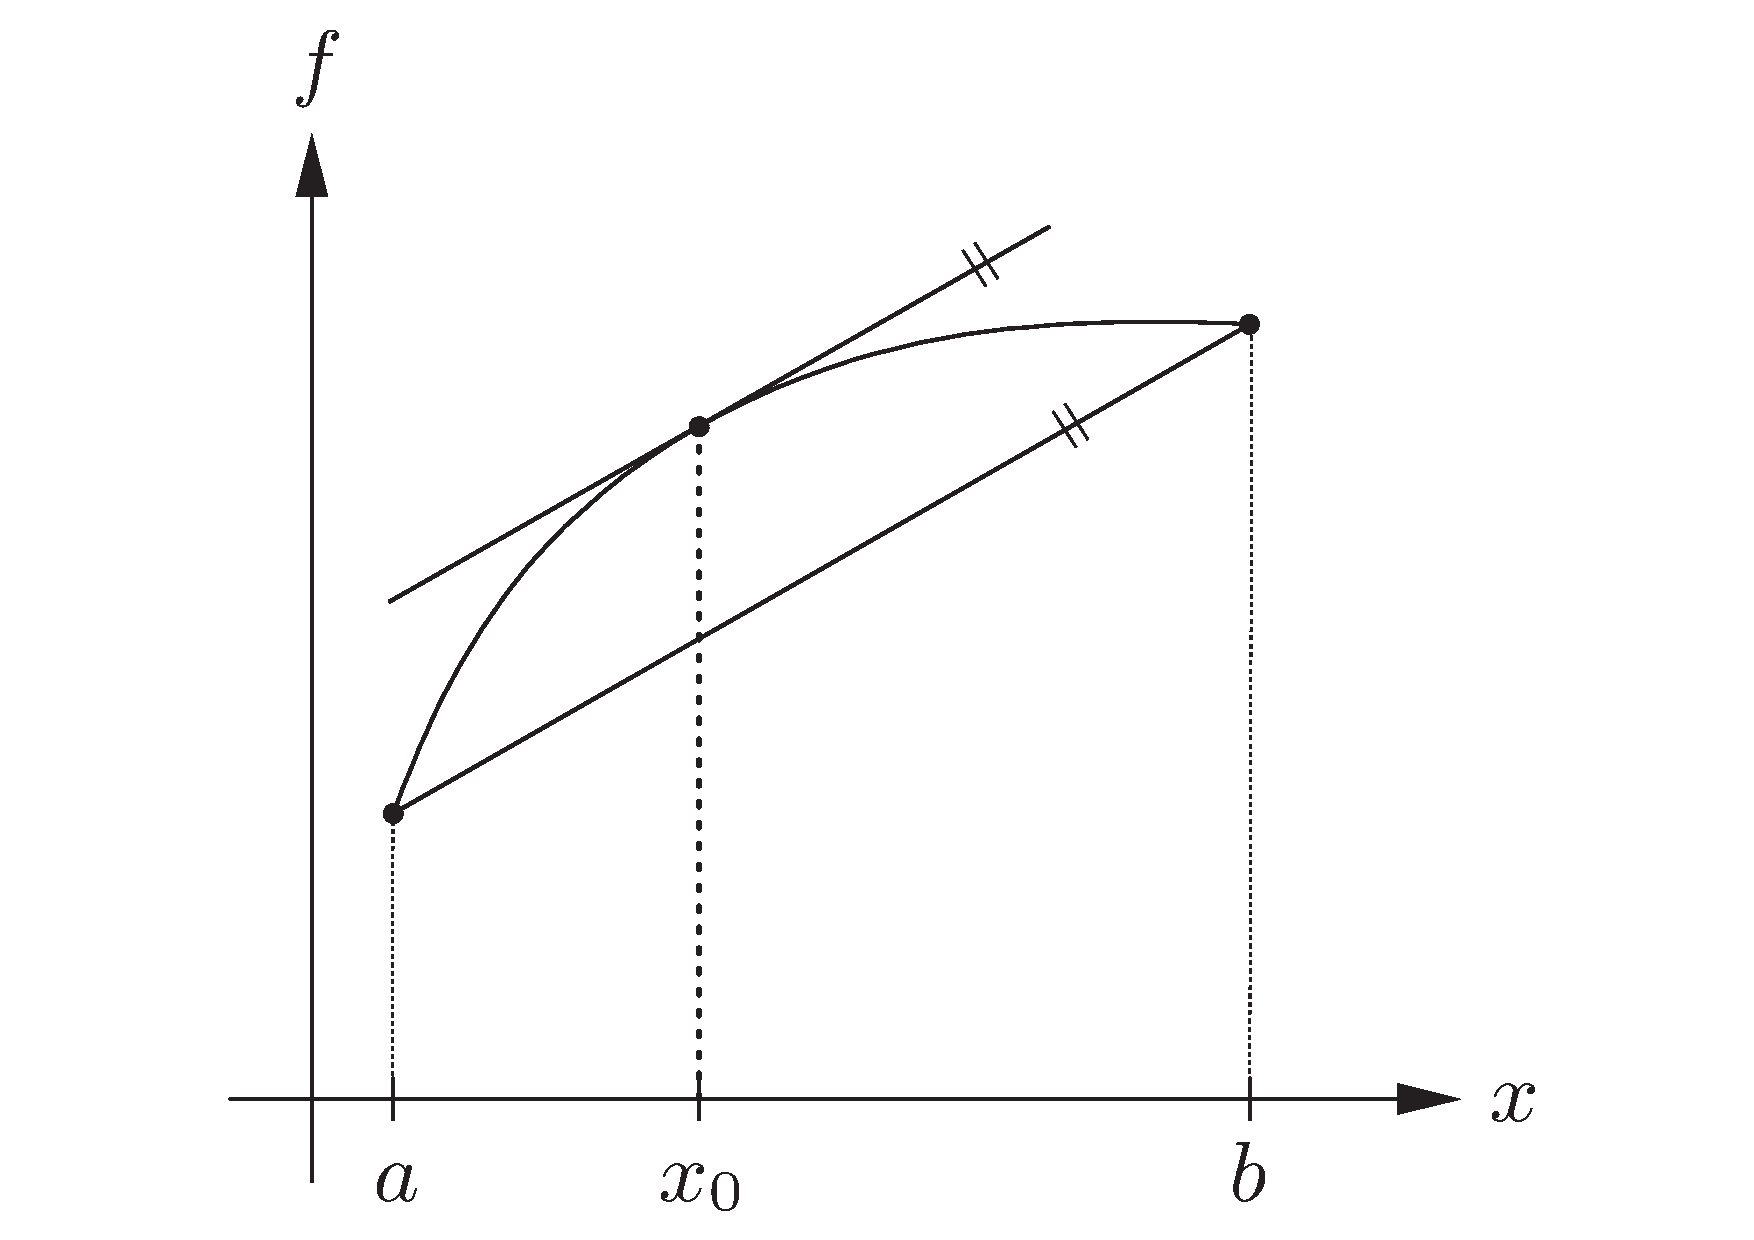
\includegraphics[width=0.7\linewidth]{img/mws.pdf}
%\end{figure}
\end{warmup}

\Bem Das heisst, es gibt eine Stelle $c\in(a,b)$, und die Steigung in $c$ bzw.
$f'(c)$ entspricht genau dem Differenzenquotient an den Stellen $a$ und $b$.

\sep

\textbf{Beweise anhand des Mittelwertsatzes}

\Vorgehen Man Formt was zu beweisen ist um, in eine Gleichung, die der des MWS
entspricht.

\Vorgehen Bei Beweisen mit dem MWS versucht man das Intervall geschickt zu
wählen (beliebige Punkte, oder spezifische Ausdrücke), so dass beim Anwenden des
MWS eine Gleichung entsteht, die der Gleichung, die zu beweisen ist, schon sehr
ähnlich ist. Dann muss man eventuell noch abschätzen, und umformen um die zu
zeigende Gleichung zu erhalten. Bei einfacheren Aufgaben, geht es einfach darum
die MWS-Gleichung aufzustellen und daraus Eigenschaften von einer Funktion
abzuleiten. In selteneren Fällen muss man eine Hilfsfunktion aufstellen.

\begin{warmup}
\sep

\Bsp Sei $f\colon [a,b]\to\R$ stetig und auf $(a,b)$ differenzierbar. Beweise
das folgende Kriterium
\[
\forall x \in(a,b) \ f'(x)=0 \Longrightarrow f(x) \text{ ist auf } (a,b)
\text{ konstant.}
\]
Seien $x_1,x_2$ beliebige Punkte in $(a,b)$, wobei $x_1<x_2$. Gemäss des
Mittelwertsatzes muss es also ein $c\in(x_1,x_2)$ geben, so dass folgendes gilt.
\[
f'(c) = \frac{f(x_2)-f(x_1)}{x_2-x_1}
\]
Wir beweisen die Implikation direkt, somit gilt gemäss Annahme $\forall x
\in(a,b) \ f'(x)=0$, insebsondere also auch $f'(c)=0$. Woraus folgt
\[
0 = \frac{f(x_2)-f(x_1)}{x_2-x_1}
\]
Das bedeutet, dass gilt $f(x_2) = f(x_1)$. Da $x_1$ und $x_2$ beliebige Punkte
auf $(a,b)$ sind, folgt, dass $f$ konstant ist.

\sep

\Bsp Gibt es eine differenzierbare Funktion $f$ mit $f(0)=-1$ und $f(2)=4$ und
$f(x)\leq 2$ für alle $x$?
\[
f \text{ diff'bar} \Longrightarrow f \text{ stetig}, \text{insbesondere auf }
[0,4]
\]
Gemäss dem MWS muss gelten $\exists c\in (0,4)$, sodass
\[
f'(c) = \frac{f(2)-f(0)}{2-0} = \frac{4 -(-1)}{2} = \frac{5}{2} > 2.
\]
Daraus folgt, dass keine solche Funktion $f$ existieren kann.

\sep

\Bsp Zeige: $\abs{\sin(a) - \sin(b)} \leq \abs{a-b}$.

Sei $f(x)=\sin(x)$, dann gilt gemäss dem MWS für beliebige $a,b\in R$ $a<b$,
dass ein $c\in(a,b)$ existiert, sodass
\[
f'(c) = \cos(c) = \frac{\sin(a) - \sin(b)}{a-b}
\]
Die die Gleichung immer gilt, muss sie insbesondere auch im Betrag gelten, also
folgt
\[
\abs{\cos(c)} =  
\abs{\frac{\sin(a) - \sin(b)}{a-b}}
\]
Da $\abs{\cos(c)}\leq 1$ folgt
\[
1\geq \abs{\cos(c)} =   
\abs{\frac{\sin(a) - \sin(b)}{a-b}}
\]
\[
1\geq \frac{\abs{\sin(a) - \sin(b)}}{\abs{a-b}}
\Longleftrightarrow
\abs{a-b} \geq \abs{\sin(a) - \sin(b)}
\]

\sep

\Bsp Zeige $\frac{1}{n^{\alpha+1}} <
\frac{1}{\alpha}\left(\frac{1}{(n-1)^\alpha} - \frac{1}{n\alpha}\right)$ für
$n\in N$ und $\alpha > 0$ (Hinweis: Betrachte die Funktion
$\frac{1}{x^\alpha}$).

Wir zeigen das mit dem Mittelwertsatz. Dazu wählen wir die Randpunkte,
geschickt, so dass sich durch umformen die zu zeigende Gleichung ergibt.

Wir betrachten die Funktion $f(x)=\frac{1}{x^\alpha}$ auf dem Intervall
$[n-1,n]$. Diese Funktion ist auf $[n-1,n]$ stetig und auf $(n-1,n)$
differenzierbar. Die Ableitung ist $f'(x)=-\frac{\alpha}{x^{\alpha +1}}$.

Das geschickte wählen des Intervalls hilft uns jetzt: Nach dem Mittelwertsatz
gibt es ein $c\in[n-1,n]$ mit
\[
f'(c) = -\frac{\alpha}{c^{\alpha +1}} = \frac{f(n)-f(n-1)}{n-(n-1)} =
\frac{1}{n^\alpha}-\frac{1}{(n-1)^\alpha}.
\]
Nun müssen wir folgende Gleichung geschickt umformen.
\begin{align*}
-\frac{\alpha}{c^{\alpha +1}} &= \frac{1}{n^\alpha}-\frac{1}{(n-1)^\alpha}
\\
\frac{\alpha}{c^{\alpha +1}} &= \frac{1}{(n-1)^\alpha}-\frac{1}{n^\alpha}
\\
\frac{1}{c^{\alpha +1}} &=
\frac{1}{\alpha}\left(\frac{1}{(n-1)^\alpha}-\frac{1}{n^\alpha}\right)\\
\end{align*}
Da $c\in(n-1,n)$ gilt $c<n$, also gilt $\frac{1}{n}<\frac{1}{c}$, und
somit
\[\frac{1}{n^{\alpha +1}}<
\frac{1}{c^{\alpha +1}} =
\frac{1}{\alpha}\left(\frac{1}{(n-1)^\alpha}-\frac{1}{n^\alpha}\right).
\]

\sep

\Bsp Beweise das folgende Kriterium für Monotonie: Gilt $f'(x)>0$ für alle
$x\in(a,b)$, so ist $f$ auf $(a,b)$ monoton wachsend.

Es seien $x_1<x_2$ zwei beliebige Punkte in $(a,b)$. Zu zeigen ist, dass
$f(x_2) > f(x_1)$ gilt. Nach dem Mittelwertsatz existiert ein $c\in(x_1,x_2)$,
sodass
\[
0 \stackrel{\text{p. Def.}}{<} f'(c) =
\frac{f(x_2)-f(x_1)}{\underbrace{x_2-x_1}_{>0}}
\Longrightarrow
f(x_2) - f(x_1) > 0.
\]
\[
\Longrightarrow f(x_2) > f(x_1).
\]
Da $x_1$ und $x_2$ beliebig sind, ist die Funktion streng monoton wachsend.

\sep

\Bsp Sei $f\colon[a,b]\to\R$ auf $[a,b]$ stetig und auf $(a,b)$ differenzierbar.
Es gelte $f'(x)\leq C$ für alle $x\in(a,b)$. Zeige, dass für alle $x\in(a,b)$
gilt:
\[
f(x)\leq f(a) +C(x-a).
\]
Wieder geht es darum das Intervall auf dem der MWS angewendet werden soll
geschickt zu wählen, so dass praktisch eine Gleichung entsteht, wie die die zu
beweisen ist. Sei $x\in(a,b)$, dann gilt gemäss des MWS, dass ein $c\in(x,a)$
eistiert, sodass
\[
f'(c) = \frac{f(x)-f(a)}{x-a} \Longrightarrow f(x) -
f(a) = f'(c)(x-a)\\
\]
\[
\Longrightarrow
f(x) =f(a) + \underbrace{f'(c)}_{\leq C}(x-a) \leq f(a) + C(x-a).
\]

\sep

\todo Evtl. noch Bernoulli-de l'Hôpital Bsp aus Buch

\todo Evtl. noch Beispiele aus den Übungen (oder Prüfungen).
\end{warmup}

\newpage

\section{14. Die Taylorschen Formeln}

Ziel dieses Kapitels ist die Approximation von $C^m$-Funktionen mithilfe von
Polynomen.

\subsection{14.1 Das Taylorpolynom und die Taylorsche Formel}

\Def Das Polynom
\[
P^{a}_m	(x):= f(a) + f'(a)(x-a) + \cdots + \frac{1}{m!} f^{(m)}(a)(x-a)^m
\]
\[
P^{a}_m	(x):= \sum_{k=0}^m \frac{1}{k!} f^{(k)}(a) (x-a)^k
\]
heisst \emph{Taylorpolynom }$m$\emph{-ter Ordnung} von $f(x)$ an der Stelle
$x=a$. Wir erwarten, dass die Funktion $f(x)$ umso besser vom Taylorpolynom
$P^{a}_m$ approximiert wird, je mehr Ableitungen der beiden Funktionen an der
Stelle $a$ übereinstimmen, d.h. je grösser $m$ ist. Wir sind hauptsächlich am
Fehler beider Approximation interessiert.
Dieser Fehler ist durch den $m$\emph{-ten Restterm} gegeben
\[
R^{a}_m (x) := f(x)-P^{a}_m(x).
\]

\sep

\Satz (Taylorsche Formel $n$-ter Ordnung) Sei $f\in C^m([a,b])$ auf $(a,b)$
$m+1$-mal differenzierbar. Dann existiert ein $\xi\in(a,b)$ mit
\[
f(x) = P^{a}_m	(x) + \frac{1}{(m+1)!}f^{(m+1)}(\xi)(x-a)^{m+1}
\]

\Bem Die Taylorsche Formel liefert somit eine Approximation einer Funktion durch
ein Polynom vom Grad $m$ und liefert eine explizite Formel für den Fehlerterm
\[
R^{a}_m(x) = \frac{1}{(m+1)!}f^{(m+1)}(\xi)(x-a)^{m+1},
\]
wobei $\xi$ eine Zahl ist, welche zwischen $a$ und $b$ liegt.

\begin{warmup}
\sep

\Bsp (Entwicklung) Bestimme das Taylorpolynom 3. Ordnung von $f(x)$ an der
Stelle $a=\frac{\pi}{2}$ und gib eine Abschätzung für den Restterm in der
Umgebung $[0,\pi]$ an.
\[
f(x)=e^x\cdot \sin(x)
\]
Dazu bilden wir zuerst die Ableitungen bis und mit zur $m$-ten Ableitung und
werten dann die Ableitungen an der Stelle $a=\frac{\pi}{2}$ aus.
\begin{align*}
&f(x)=e^x\cdot \sin(x) &&\Longrightarrow f(\pi/2)=e^{\frac{\pi}{2}}\\
&f'(x)=e^x\cdot(\sin(x) + \cos(x)) && \Longrightarrow f'(\pi/2)=e^{\frac{\pi}{2}}\\
&f^{\prime\prime}(x)=2e^x\cdot(\cos(x)) && \Longrightarrow f^{\prime\prime}(\pi/2)=0\\
&f^{\prime\prime\prime}(x)=2e^x\cdot(\cos(x) + \sin(x)) && \Longrightarrow
f^{\prime\prime\prime}(\frac{\pi}{2}) =2e^{\frac{\pi}{2}}
\end{align*}
Nun können wir das Taylorpolynom 3. Ordnung an der Stelle $\frac{\pi}{2}$
aufschreiben:
\[
P^{\frac{\pi}{2}}_3(x)=e^{\frac{\pi}{2}} + e^{\frac{\pi}{2}}(x-\frac{\pi}{2}) 
+ 2e^{\frac{\pi}{2}}\frac{(x-\frac{\pi}{2})^3}{3!}
\]
\[
=e^{\frac{\pi}{2}}\left(1 + x - \frac{\pi}{2}
+\frac{1}{3}(x-\frac{\pi}{2})^3\right)
\]
Der Restterm ist in der Umgebung $[0,\pi]$ folgendermassen beschränkt
\[
\abs{R^{\frac{\pi}{2}}_3(x)} = \abs{f(x)-P^{\frac{\pi}{2}}_3(x)}
\]
\[
=\abs{e^x\cdot\sin(x) - e^{\frac{\pi}{2}}\left(1 + x - \frac{\pi}{2}
+\frac{1}{3}(x-\frac{\pi}{2})^3\right)}
\leq \cdots
\]
(Die Abschätzung ist in diesem Fall etwas kompliziert und wurde deshalb
ausgelassen.)

\sep

\Bsp (Entwicklung, Fehlerabschätzung) Bestimme mit Hilfe des linearen
Taylorpolynoms um $t_0=8$ eine Näherung an $\sqrt[3]{7}$. Gib eine Abschätzung
für den Fehler dieser Näherung an.

Für $f(t)=\sqrt[3]{x}=t^{\frac{1}{3}}$ ist $f'(t)=\frac{1}{3}t^{-\frac{2}{3}}$.
$\Longrightarrow$ Lineares Taylorpolynom um $t_0=8$:
\[
P_1f(t)=f(8) + f'(8)(t-8) = 2 + \frac{1}{3}\cdot\frac{1}{4}\cdot(t-8)
\]
Also Näherung für $\sqrt[3]{7}$:
\[
P_1(7) = 2+\frac{1}{3}\cdot\frac{1}{4}\cdot(7-8) = \frac{23}{12}. 
\]
Fehlerabschätzung:
\[
R_1(7) = \frac{f^{\prime\prime}(\xi)}{2!}(t-t_0)^2 
= \frac{f^{\prime\prime}(\xi)}{2!}(7-8)^2
\]
für ein $\xi\in[7,8]$.

Aus $f^{\prime\prime}(x)=-\frac{2}{9}t^{-\frac{5}{3}}$ folgt
\[
R_1(7) \leq \frac{ \sup_{\xi\in[7,8]}\abs{f^{\prime\prime}(\xi)}}{2!}(7-8)^2
= \frac{\frac{2}{9}7^{-\frac{5}{3}}}{2}
= \frac{1}{9\cdot\sqrt[3]{7^5}}.
\]

\sep
\end{warmup}

\begin{warmup}
\subsection{14.2 Taylorreihen und analytische Funktionen}

Ist die Funktion $f\colon\Omega\subset\R\to\R$ in der Nähe von $a$ unendlich oft
differenzierbar, so wird die Reihe
\[
P(x) = \sum_{n=0}^{\infty} \frac{1}{n!}f^{(n)}(a)(x-a)^n
\]
die \emph{Taylorreihe} von $f$ um $x=a$ genannt. Die Taylorreihe von $f$ um $a$
ist eine Potenzreihe in $(x-a)$, also um den Punkt $a$ zentriert. Sie braucht nicht
unbedingt für alle $x\in\Omega$ zu konvergieren. Sondern sie besitzt einen
eigenen Konvergenzradius $\rho$, den man mit den üblichen Regeln für
Potenzreihen bestimmen kann, und konvergiert entsprechend auf einer Umgebung von
$a$, welche dem Konvergenzbereich der Potenzreihe entspricht.

Wenn sie ausserdem auch konvergiert, muss die Taylorreihe von $f$ an der Stelle
$x$ nicht notwendigerweise gegen die Funktion $f(x)$ konvergieren. Zum Beispiel
ist
\[
\sum_{n=0}^\infty x^n
\]
die Taylorreihe zur Entwicklungsstelle $a=0$ für die Funktion
$f(x)=\frac{1}{1-x}$. Obwohl die Funktion $f(x)$ für alle $x\neq 1$ definiert
ist, konvergiert die Taylorreihe nur für $\abs{x}<1$ gegen $f(x)$. Für
$\abs{x}\geq 1$ divergiert sie und stellt dort somit nicht die Funktion $f(x)$
dar.

\todo schauen ob der Rest noch relevant wird.

\end{warmup}

\newpage

\section{15. Folgen stetiger Funktionen}

\Def Eine \emph{Folge stetiger Funktionen} ist eine Folge
$f_n\colon\Omega\subset\R\to\R$, deren Folgenglieder $f_n$ stetige Funktionen
auf $\Omega$ sind.

\Bem Für jedes $n$ haben wir also eine stetige Funktion von $x$.

\Bem Die Fragen, die entstehen sind: Für welche $x\in\Omega$ konvergiert
$f_n(x)$? Wie sieht die Grenzfunktion $\lim_{n\to\infty} f_n(x)=:f(x)$ aus?
Unter welchen Bedingungen ist $f(x)$ stetig? Was ist der Wert von
$\lim_{n\to\infty}\int_\Omega f_n(x) dx$?

\Bem Diese Konzepte erlauben uns Tricks anzuwenden wie z.B. das Integral und den
Limes in der obigen Berechnung zu vertauschen (nur erlaubt, falls $f_n$ auf
$\Omega$ gleichmässig konvergiert), womit die obige Berechnung mit einem
reduzierten Rechenaufwand durchgeführt werden kann.

\sep

\subsection{15.1 Punktveise vs. Gleichmässige Konvergenz}

\Def Eine Folge stetiger Funktionen $f_n\colon\Omega\subset\R\to\R$
\emph{konvergiert punktweise} gegen $f(x)$, falls
\[
\forall x\in\Omega \ \lim_{n\to\infty} f_n(x) = f(x).
\]
Die Grenzfunktion $\lim_{n\to\infty} f_n(x) = f(x)$ heisst \emph{punktweiser}
Limes der Folge $f_n(x)$.

\Bem um eine vorgelegte Folge stetiger Funktionen auf punktweise Konvergenz zu
überprüfen, muss man also einfach $x$ festhalten und den Limes von $f_n(x)$ für
$n\to\infty$ berechnen.

\Bem Die punktweise Konvergenz ist der natürlichste Konvergenzbegriff, er ist
aber nicht stark genug, um Limes und Integral vertauschen zu dürfen. Deshalb hat
man noch den etwas stärkeren Konvergenzbegriff der gleichmässigen Konvergenz
eingeführt.

\sep

\Def Eine Folge stetiger Funktionen $f_n\colon\Omega\subset\R\to\R$
\emph{konvergiert gleichmässig} gegen $f$, falls
\[
\lim_{n\to\infty} \sup_{x\in\Omega} \abs{f_n(x)-f_n(y)} = 0.
\]

\Bem Die gleichmässige Konvergenz impliziert die punktweise Konvergenz.

\sep

\Satz Sei $f_n\colon\Omega\subset\R\to\R$ eine Folge stetiger Funktionen. Falls
$f_n$ gegen $f$ gleichmässig konvergiert, ist $f$ stetig.

\Bem Der Satz ist in seiner Umkehrung oft sehr nützlich.

\sep

\Satz (Dini) Sei $f_n\colon\Omega\subset\R\to\R$ eine Folge stetiger Funktionen
mit punktweisem Limes $f$ und sei $\Omega$ kompakt. Ist $f$ stetig und $f_n$
monoton wachsend, so konvergiert $f_n$ gleichmässig gegen $f$.

\begin{warmup}
\todo Brauche ich den Satz?
\end{warmup}


\sep

\Def Eine \emph{monoton wachsende Folge von stetigen Funktionen} ist eine Folge
$f_n(x)$, für welche $f_n(x)\leq f_{n+1}(x)$ für alle $x\in\Omega$ gilt.

\Achtung Das heisst nicht dass $f_n$ jeweils monoton wachsend ist.

\sep

\textbf{Kochrezept für Gleichmässige Konvergenz}

Gegeben: Folge stetiger Funktionen: $f_n\colon\Omega\subset\R\to\R$.

Gefragt: Konvergiert $f_n$ auf $\Omega$ gleichmässig?

\textbf{Schritt 1:} Berechne den punktweisen Limes von $f_n$ auf $\Omega$, d.h.
\[
f(x) = \lim_{n\to\infty} f_n(x) \quad \text{für fixes }x\in\Omega
\]

\textbf{Schritt 2:} Prüfe $f_n$ auf gleichmässige Konvergenz.

\underline{Direkte Methode:}
\begin{enumerate}[label=\roman*)]
  \item Berechne
  \[
  	\sup_{x\in\Omega} \abs{f_n(x)-f(x)}.
  \]
  Zu diesem Zweck ist es oft nützlich, die Ableitung nach $x$ von
  $\abs{f_n(x)-f(x)}$ zu berechnen und diese gleich Null zu setzen.
  \item Bilde den Limes für $n\to\infty$
  \[
  \lim_{n\to\infty} \sup_{x\in\Omega} \abs{f_n(x)-f(x)}.
  \]
  Gilt $\lim_{n\to\infty} \sup_{x\in\Omega} \abs{f_n(x)-f(x)}=0$, so ist $f_n$
  auf $\Omega$ gleichmässig konvergent.
\end{enumerate}

\underline{Indirekte Methoden:}
\begin{itemize}
  \item $f$ unstetig $\Longrightarrow$ keine gleichmässige Konvergenz.
  \item $f$ stetig, $f_n(x)\leq f_{n+1}(x) \ \forall x\in\Omega$ und $\Omega$
  kompakt $\Longrightarrow$ gleichmässige Konvergenz.
\end{itemize}

\begin{warmup}
\sep

\todo Beispiele

\todo Eventuell werden die folgenden Kapitel später relevant.
\end{warmup}


\newpage

\part{Integralrechnung in $\R$}

Die Integralrechnung hat zwei Aspekte:
\begin{itemize}
  \item Integrieren als Umkehrung des Differenzierens mit einer
  Funktion(sklasse) als Ergebnis
  \item Bestimmte Integrale mit einem Zahlenwert als Ergebnis
\end{itemize}

\section{16. Unbestimmte Integrale}

\Def Das Integrieren als Umkehrung des Differenzierens ist das \emph{Aufsuchen
einer Stammfunktion} $F$ zu einer gegebenen \emph{stetigen} Funktion $f$,
sodass $F'(x)=f(x)$ für alle $x$ im Definitionsberech von $f$ gilt. Es wird also eine
Funktion $F$ gesucht, deren Ableitung gerade die vorgelegte Funktion $f$ ist.
Die Funktion $F$ wird als Stammfunktion von $f$ bezeichnet und symbolisch wird
\[
F(x) = \int f(x) \ dx = \int F'(x) \ dx
\]
geschrieben. Beim Integrieren tritt immer eine \emph{Integrationskonstante}
$C\in\R$ auf, da mit $F$ auch $F+C$ eine Stammfunktion ist.

\sep

\subsection{16.1-16.2 Elementare Integrale}

Elementare Integrale, lassen sich durch Umkehrung der Ableitung
direkt angeben.

\begin{table}[H]
\centering
\begin{tabular}{|c|c|}
\toprule
$f(x)$ & $F(x)$ \\
\midrule
$x^\alpha$, $(\alpha\neq 0)$ & $\frac{x^{\alpha +1}}{\alpha +1}+C$
\\
$\frac{1}{x}$ & $\ln(\abs{x})+C$
\\
\hline
$e^x$ & $e^x + C$
\\
$\alpha^x$ & $\frac{\alpha^x}{\ln(\alpha)}+C$
\\
\hline
$\sin(x)$ & $-\cos(x)+C$
\\
$\cos(x)$ & $\sin(x)+C$
\\
\hline
$\sinh(x)$ & $\cosh(x) + C$
\\
$\cosh(x)$ & $\sinh(x) + C$
\\
\hline
$\frac{1}{\sqrt{1-x^2}}$ & $\arcsin(x)+C$
\\
$\frac{-1}{\sqrt{1-x^2}}$ & $\arccos(x)+C$
\\
$\frac{1}{1+x^2}$ & $\arctan(x)+C$
\\
\hline
$\frac{1}{\sqrt{1 + x^2}}$ & $\arcsinh(x)+C$
\\
$\frac{1}{\sqrt{x^2-1}}$ & $\arccosh(x)+C$
\\
$\frac{1}{1-x^2}$ & $\arctanh(x)+C$
\\
\hline
$\tan(x)$ & $-\log(\abs{\cos(x)})+C$\\
\hline
$\log(x)$ & $x(\log(x)-1)+C$\\
\bottomrule
\end{tabular}
\end{table}

Weiss nicht, ob ich diese verwenden darf:

\[\int \cos (x) \sin ^n(x) \, dx=\text{constant}+\frac{\sin ^{n+1}(x)}{n+1}\]
\[\int \sin (x) \cos ^n(x) \, dx=\text{constant}-\frac{\cos ^{n+1}(x)}{n+1}\]


\subsection{16.3 Direkte Integrale}

\Def Direkte Integrale sind Integrale der Form
\[
\int f(g(x))g'(x) \ dx
\]
\[
\int (f \text{ ausgewertet in } g) \cdot (\text{Ableitung von } g(x)) \ dx.
\]
wobei $f$ eine \emph{stetige} und $g$ eine \emph{differenzierbare} Funktion ist.

\Bem Wir können eine allgemeine Formel für solche Integrale mittels der
Kettenregel bekommen. Ist $F$ eine Stammfunktion von $f$ so gilt nach der Kettenregel
\[
(F\circ g)'(x) = F'(g(x))\cdot g'(x) = f(g(x))\cdot g'(x).
\]

\Satz Hat der Integrand die Form $f(g(x))\cdot g'(x)$, so gilt unmittelbar
folgendes
\[
\int f(g(x))\cdot g'(x) \ dx = F(g(x))
\]
\[
\qquad = \text{Stammfunktion von } f \text{ in }
g(x) \text{ ausgewertet.}
\]

\sep

\Vorgehen Man versucht das Integral in ein Produkt $\int f(g(x))\cdot g'(x) \
dx$ zu zerlegen, integriert dann $f(x)$ und bekommt $F(x)$. Danach setzt man
$g(x)$ ein und erhält $\int f(g(x))\cdot g'(x) \ dx = F(g(x))+ C$:

\Trick Es gibt mehrere Tricks:
\begin{itemize}
  \item Ein Muster aus den Elementaren Integralen erkennen
  \item $0$ addieren
  \item Mit $1$ multiplizieren, einmal innerhalb und ausserhalb des Integrals,
  um den gewünschten Faktor im Nenner oder Zähler zu erhalten.
  \item Integral in zwei Integrale aufteilen
\end{itemize}

\begin{warmup}
\Bsp
\todo 2 3 Beispiele
\end{warmup}

\sep

\subsection{16.4 Partielle Integration}

Die partielle Integration erlaubt die Integration von Produkten. Die parteille
integration ergibts sich aus der Umkehrung der Produktregel der
Differenzialrechnung:

\Satz \todo Prerequisites ($g$ diffbar?) 
\[
\int f'\cdot g \ dx = f\cdot g - \int f \cdot g' \ dx
\]
Achtung, bei einem bestimmten Integral darf man nicht vergessen das bestimmte
Integral von $[f\cdot g]_a^b$ zu bilden:
\[
\int_a^b f'\cdot g \ dx = \left[f\cdot g\right]_a^b - \int_a^b f\cdot g' \ dx
\]

\sep

\Vorgehen Für die Berechnung von $\int F(x) \ dx$ mittels partieller Integration
versucht man, den Integranden als Produkt von zwei Funktionen
\[
F = f'\cdot g
\]
zu schreiben, wobei nun die Funktion $f'$ integriert $(\uparrow)$ und $g$
abgeleitet $(\downarrow)$ wird. Wie genau man erkennt, welche Funktion die Rolle
von $f'$ und welche die von $g$ einnimmt, hängt stark von der Situation ab. Es
gibt keine allgemeine Regel. Für die meisten Situationen kann folgende Tabelle
hilfreich sein:

\vspace{5pt}

\resizebox{\columnwidth}{!}{
\begin{tabular}{l|p{5.5cm}}
\toprule
$(\uparrow)$, bzw. $f':=$ & 1 (falls $\arc$-Funktion oder Logarithmus vorkommt),
$x^n$, $\frac{1}{1-x^2}$, $\frac{1}{1 + x^2}$, \ldots
\\
\hline
$(\downarrow)$, bzw. $g:=$ & $x^n$, $\log(x)$, $\arcsin(x)$, $\arccos(x)$,
$\arctan(x)$, $\arcsinh(x)$, $\arccosh(x)$, $\arctanh(x)$, \ldots
\\
\hline
``egal'' & $e^x$, $\sin(x)$, $\cos(x)$, $\sinh(x)$, $\cosh(x)$, \ldots
\\
\bottomrule
\end{tabular}
}
\vspace{3pt}

Danach schreibt man sich $f'(x)$ und $g(x)$ nebeneinander hin und wendet die
operationen an:
\begin{align*}
&f'(x):= \ldots \qquad &&g(x):= \ldots\\
&(\uparrow \text{ integrieren}) \qquad && (\downarrow \text{ ableiten})\\
&f(x) :=	\ldots \qquad && g'(x) := \ldots \\
\end{align*}

Nachdem man $f(x)$ und $g'(x)$ ausgerechnet hat, schreibt man sich durch
einsetzen den rechten Teil dieser Gleichung hin.
\[
\int f'\cdot g \ dx = f\cdot g - \int f \cdot g' \ dx
\]

Das Ziel der ganzen Sache, ist, dass das zweite integral (rechts) einfacher
wird, und es sich somit einfacher als das ursprüngliche bestimmen lässt (evtl.
auch erst nach ein paar Schritten).

\Trick Zum Lösen partieller Integrale gibt es eine Reihe verschiedener
Tricks:

\begin{itemize}
  \item Quadrate, oder Potenzen in Produkt zerlegen, um Produkt zu erhalten
  \item Bei komplizierten Funktionen (wie z.B. $\log$, $\arcsin$, \ldots) mit
  $1$ multiplizieren und $f'=1$ nehmen.
  \item Substitution mit durch trigonometrische Identitäten
  \item Partielle Integration mehrmals anwenden, bis sich das Integral auflösen
  lässt, oder bis man wieder das ursprüngliche Integral erhält, und es per
  Auflösen der Gleichung erhalten kann (eg. $I = \ldots - I \longrightarrow 2I
  = \ldots \longrightarrow I=\frac{1}{2}(\ldots)$).
\end{itemize}

\begin{warmup}
\sep

\Bsp \todo 2-3 Beispiele
\end{warmup}


\subsection{16.6 Die Substitutionsregel}

Hierbei versucht man die Variablen und evtl. vorhandenen Integrationsgrenzen
durch eine abhängige Variable zu ersetzen, so dass das Integral einfacher zu
lösen wird.

Die Idee der Substitution besteht darin, eine Variablentransformation
\[
y = g(x)	\Longleftrightarrow x = g^{-1}(y)
\]
durchzuführen. Dabei ist $g$ ein Diffeomorphismus, d.h. eine in beiden
Richtungen stetig differenzierbare Abbildung.

\sep

\Satz \textbf{Substitutionsregel} Ist $f$ stetig und $g$ wie oben, dann gilt
\[
\int f(g(x))g'(x) \ dx = \int f(y) \ dy
\]

\Bem Die Substitutionsregel folgt unmittelbar aus der Kettenregel.

\sep

\Vorgehen Falls wir die Schreibweise mit dem ``$dx$'' für die Ableitung von $g$
benutzen
\[
\frac{dy}{dx} = g'(x) \Longleftrightarrow dy = g'(x) dx
\]
gilt folgender Merksatz: Um $\int f(y) \ dy$ zu berechnen substituiere $y=g(x)$
im Integrand und ersetzte das ``$dy$'' mit ``$g(x)dx$'' mit dem Ziel, dass das
neue Integral $\int f(g(x))\cdot g'(x) \ dx$ leichter zu bestimmen ist als das
ursprüngliche. Nach dem Integrieren muss man wieder für $y$ die Ursprüngliche
Funktion $g(x)$ einsetzen d.h. rücksubstituieren.

\sep

\Vorgehen Oft beginnt man mit einem Integral, und substituiert dann einen Teil
\[
\int \ldots\text{eins odere mehreren } g(x) \text{ erscheinen} \ldots \ dx
\]
Substitution von $g(x)$ durch $y$:
\begin{align*}
y = g(x) \Longleftrightarrow \qquad x&=g^{-1}(y)\\
dx &= g^{-1\prime}(y) dy\\
\end{align*}
Man ersetzt also $x$ mit $g^{-1}(y)$ und $dx$ mit $g^{-1\prime}(y) dy$. Danach
löst man das Integral nach $y$ (evtl. mit noch einem anderen Verfahren) und 
substituiert dann irgendwann alle $y$ mit $y=g(x)$ zurück, so dass ein Ausdruck
abhängig von $x$ entsteht.

\sep

\Trick Welche Substitution sich jeweils am besten eignet zeigen wir anhand von
typischen Situationen.

Integrale von Funktionen, die \{\{Ausdruck\}\} enthalten löst man oft mit der
Substitution:
\begin{itemize}[label=$\star$]
\item $e^x$, $\sinh(x)$, $\cosh(x)$, \ldots:
\[
e^x = t \qquad (dx = \frac{1}{t} dt)
\]
\item $\log(x)$:
\[
\log(x) = t, \qquad (dx = e^t dt)
\]
\item $\sqrt[\alpha]{Ax + B}$:
\[
\sqrt[\alpha]{Ax + B} = t \Rightarrow Ax + B = t^2
\]
\item $\cos(x)$, $\sin(x)$ in geraden Potenzen oder $\tan(x)$:
\[
\tan(x) = t \qquad \left(dx = \frac{1}{1 + t^2} dt \right)
\]
Für $\sin(x)$ und $\cos(x)$ wird dann entsprechend substitutiert. Man bildet
dann damit einfach höhere Potenzen falls man es braucht.
\[
\sin^{2}(x)=\frac{t^2}{1+t^2}
\qquad 
\cos^2(x) = \frac{1}{1 + t^2}
\]
\item $\cos(x)$, $\sin(x)$ in ungeraden Potenzen:
\[
\tan\left(\frac{x}{2}\right) = t \qquad \left(dx = \frac{2}{1 + t^2} dt\right)
\]
Entsprechend wird für $\sin(x)$ und $\cos(x)$ folgendermassen substitutiert:
\[
\sin(x) = \frac{2t}{1 + t^2}
\qquad
\cos(x) = \frac{1-t^2}{1 + t^2}
\]
\item $\sqrt{Ax^2 + Bx + C}$ im Nenner:\\
Mittels quadratischer Ergänzung werden diese Integrale auf einen der folgenden
Fälle zurückgeführt:
\[
\int \frac{1}{\sqrt{1 - x^2}} \ dx = \arcsin(x) + C,
\]
\[
\int \frac{1}{\sqrt{1+x^2}} \ dx = \arcsinh(x) + C.
\]
\[
\int \frac{1}{\sqrt{x^2-1}} \ dx = \arccosh(x) + C,
\]

\item $\sqrt{Ax^2 + Bx + C}$ im Zähler:\\
Mittels quadratischer Ergänzung werden diese Integrale auf einen der folgenden
Formen gebracht und dann mithilfe der folgenden Substitutionen gelöst:
\[
\int \sqrt{1-x^2} \ dx \qquad \text{Substitution } x= \sin(t)
\]
\[
\int \sqrt{1+x^2} \ dx \qquad \text{Substitution } x= \sinh(t)
\]
\[
\int \sqrt{x^2-1} \ dx \qquad \text{Substitution } x= \cosh(t)
\]

\end{itemize}

\begin{warmup}

\sep

\Bsp (Midterm, 1. Variante)
\[
\int_0^1 \frac{t^3}{\sqrt{1+t^2}} \ dt
\]
Wir führen hier die folgende Substitution durch:
\[
\begin{array}{rclcl}
z &= &1+ t^2 & \Longleftrightarrow & t^2 = z-1\\
dz &= &2t \cdot dt & \Longleftrightarrow & dt = \frac{dz}{2t}
\end{array}
\]
Jetzt setzen versuchen wir alle Ausdrücke mit $t$ geeignet durch gleichwertige
mit $z$ zu ersetzen:
\begin{align*}
\qquad &= \int_{z(0)}^{z(1)} \frac{t^3}{\sqrt{z}} \frac{dz}{2t}
= \int_{1}^{2} \frac{t^2}{\sqrt{z}} \frac{dz}{2}
= \int_{1}^{2} \frac{z-1}{\sqrt{z}} \frac{dz}{2}\\
&= \frac{1}{2} \int_{1}^{2} \frac{z}{\sqrt{z}} - \frac{1}{\sqrt{z}} \ dz
= \frac{1}{2} \int_{1}^{2} z^{\frac{1}{2}} - z^{-\frac{1}{2}} \ dz\\
&= \frac{1}{2}\left[\frac{2}{3}z^{\frac{3}{2}} -2z^{\frac{1}{2}}\right]_1^2
= \ldots = \frac{2-\sqrt{2}}{3}
\end{align*}
Das Schöne daran, wenn man die Grenzen bei der Substitution gleich mitverändert
(statt das Unbestimmte Integral auszurechnen), ist dass man nicht mehr
rücksubsituieren muss (im Gegensatz zur Situation, wenn man das unbestimmte
Integral bestimmen wrüde), sondern das Integral gleich ausrechnen kann.

\sep

\Bsp (Midterm, 2. Variante)
\[
\int_0^1 \frac{t^3}{\sqrt{1+t^2}} \ dt
\]
Wir führen hier die folgende Substitution durch:
\[
z = \sqrt{1 + t^2} \Longrightarrow z^2 = 1 + t^2 \Longleftrightarrow t^2 = z^2
-1
\]
\[
dz = \frac{1}{2\sqrt{1+t^2}} \cdot 2t \cdot dt = \frac{1}{2} \cdot t \cdot dt
\Longleftrightarrow \frac{z\cdot dz}{t} = dt
\]
Wie wir sehen, haben hier gleich die ganze Wurzel substituiert, dadurch wird das
Integral noch einfacher zu lösen:
\begin{align*}
&= \int_{z(0)}^{z(1)} \frac{t^3}{z}\cdot \frac{z \cdot dt}{t}
= \int_{1}^{\sqrt{2}}t^2 \ dz
= \int_{1}^{\sqrt{2}}z^2 -1 \ dz\\
&= \left[\frac{1}{3}z^3-z\right]_{1}^{\sqrt{2}}
= \frac{2\sqrt{2}-3\sqrt{2}}{3} - \frac{1-3}{3}
= \frac{2-\sqrt{2}}{3}
\end{align*}

\sep

\end{warmup}


\subsection{16.X Logarithmisches Integrieren}

Diese Identität ist in beiden Richtungen sehr nützlich. Zum Beispiel, wenn man
ein Integral bestimmen muss, wobei der Nenner (evtl. um einen konstanten Faktor
noch verschieden) die Ableitung des Nenners ist. Oder wenn man bei Gleichungen
$y'/y$ integriert kann man dann das dann gleich mit $\ln(y)$ ersetzen. Oder beim
Lösen von Differentialgleichungen.
\[
\int \frac{f'(x)}{f(x)} dx = \int \frac{y'}{y} dx = \ln \abs{f(x)} + C
\]
Der Beweis ist ganz einfach, da die Ableitung von der rechten Seite genau den
Integrationsterm ergibt.

\subsection{16.X Partialbruchzerlegung (PBZ)}

Falls das Zählerpolynom einen höheren Grad als das Nennerpolynome hat eine
Polynomdivison durchführen und mit mit dem Rest eine PBZ durchführen.

\begin{itemize}
  \item Einfache Nullstelle $\frac{A}{x-x_1}$
  \item $m$-fache Nullstelle $\frac{A}{(x-x_1)}+\ldots+\frac{A}{(x-x_1)^m}$
  \item Komplexe Nullstelle $\frac{Bx+C}{x^2+px+q}$
  \item $m$-fache komplexe NS: analog wie $m$-fach
\end{itemize}

Dann Ausmultiplizieren und Koeffizientenvergleich machen.

\begin{warmup}
Mithilfe der Partialbruchzerlegung lassen sich Integrale manchmal einfacher
ausrechnen.

\Vorgehen

\begin{enumerate}
  \item Falls das Polynom im Zähler einen höheren Grad hat, führen wir eine
  Polynomdivision durch und schreiben, dann den Quotienten und den Rest auf.
  Danach führen wir eine PBZ für den Rest durch.
  \item Nennerpolynom faktorisieren (Binomische Formeln, Falls 2. od. 3. Grades
  Nullstellen abspalten mit Polynomdivision)
  \item Partialbruchgleichung aufstellen. Ist im Nenner ein Polynom $n$-ten
  Grades, ist im Zähler ein Polynom $n-1$-ten Grades.
  \item Auf gemeinsamen Nenner bringen
  \item Zählergleichung aufschreiben.
  \item $x$-Werte finden, für die ein Ausdruck gleich Null ist, oder Werte
  für $x$ einsetzen, die das Auflösen nach $A$, $B$, $C$, \ldots einfacher
  machen. Zwischenresultate für $A$, $B$, $C$, \ldots können eingesetzt werden.
  \item Partialbruchzerlegung aufschreiben.
\end{enumerate}

\sep

\Bsp Bestimme die PBZ von
\[
\frac{10x^2+12x+20}{x^3-8}
\]

Der Grad des Zählers ist tiefer als der des Nenners, also können wir mit Schritt
2 weiterfahren.

Den Nenner können wir nicht so einfach faktoriseren. Wir spalten dazu mit der
Polynomdivision eine Nullstelle ($x=2$) ab.

Die Polynomdivision ergibt folgende Faktorisierung für den Nenner
\[
x^3-8 = (x-2)(x^2+2x+4)
\]
Der Faktor $(x^2+2x+4)$ ist über $\R$ nicht weiter reduzibel, also können wir
mit Schritt 3 fortfahren.
\[
\frac{10x^2+12x+20}{x^3-8} = \frac{A}{x-2} + \frac{Cx+B}{x^2+2x+4}
\]
Nun bringen wir alles auf einen gemeinsamen Nenner gemäss Schritt 4.
\[
\frac{10x^2+12x+20}{x^3-8} = \frac{A(x^2+2x+4)+(Cx+B)(x-2)}{(x-2)(x^2+2x+4)}
\]
Gemäss Schritt 5, haben wir somit die folgende Gleichung für unsere
unbekannten:
\[
10x^2+12x+20 = A(x^2+2x+4)+(Bx+C)(x-2)
\]
Wir fahren mit Schritt 6 fort
\[
x=2: \quad 10\cdot 2^2+12\cdot 2+20 = A(2^2+2\cdot 2+4)
\]
\[
\Longrightarrow A = 7.
\]
Nun wissen wir $A=7$, wir wählen $x=0$, damit nur $B$ übrig bleibgt.
\[
x=0:  \quad 20 = 7\cdot 4 -2C \Longrightarrow C=4.
\]
Nun wissen wir $A=7$, $C=4$, und wählen ein einfaches $x$, um $C$ ausrechnen zu
können.
\[
x=1: \quad 10+12+20 = 7(1+2+4)+(B+4)(-1)
\]
\[
\Longrightarrow B = 3.
\]
Somit können wir jetzt gemäss Schritt 7 unsere PBZ aufschreiben:
\[
\frac{10x^2+12x+20}{x^3-8} = \frac{7}{x-2} + \frac{4x+3}{x^2+2x+4}
\]

\sep

\Bsp Sollte man eine PBZ durchführen müssen für einen Ausdruck, wo im Nenner ein
Linearfaktor mehrmals vorkommt:
\[
\frac{3x + 4}{(x^2+2x+4)(x+4)^{10}}
\]
Dann würde die Gleichung folgendermassen aussehen:
\[
\tfrac{Ax+B}{(x^2+2x+4)} + \tfrac{C}{(x+4)} + \tfrac{D}{(x+4)^2} +
\tfrac{E}{(x+4)^3} + \cdots + \tfrac{L}{(x+4)^{10}}
\]

\sep
\end{warmup}
















\newpage

\section{17. Bestimmte Integrale}

\subsection{17.1 Definition}

\Def Sei $F(x) = \int f(x) \ dx	$ die Stammfunktion der stetigen Funktion $f$.
Das \emph{bestimmte Integral} von $f$ von $a$ bis $b$ ($a<b$) ist
\[
\int_a^b f(x) \ dx := F(b) - F(a) = \left[F(x)\right]_a^b
\]
Für $a>b$ setzt man
\[
\int_a^b f(x) \ dx = - \int_b^a f(x) \ dx
\]
Ausserdem definiert man $\int_a^a f(x) \ dx$.

\subsection{17.2 Eigenschaften}

Das bestimmte Integral erfüllt die folgenden Eigenschaften
\begin{enumerate}[label=\alph*)]
  \item Linearität:\\
  $\int_a^b (\alpha f(x) + \beta g(x)) \ dx = \alpha \int_a^b f(x) \ dx + \beta
  \int_a^b g(x) \ dx$
  \item Gebietsadditivität:\\
  $\int_a^c f(x) \ dx = \int_a^b f(x) \ dx + \int_b^c f(x) \ dx$
  \item Positivität:\\
  $\forall x\in [a,b] \colon \left( f(x)\geq 0 \Longrightarrow \int_a^b f(x)\ dx
  \geq 0\right)$
  \item Monotonie:\\
  $\forall x\in [a,b] \colon \left( f(x)\geq g(x) \Longrightarrow \int_a^b f(x)
  \ dx \geq \int_a^b g(x) \ dx \right)$
  \item Dreiecksungleichung:\\
  $\abs{\int_a^b f(x) \ dx} \leq \int_a^b \abs{f(x)} \ dx$
  \item Merksatz:\\
  Ist $f(x)$ ungerade, so gilt für alle um den Ursprung symmetrischen Integrale
  $\int_{-a}^a f(x) \ dx = 0$.
\end{enumerate}

\newpage

\begin{warmup}
\sep

\Bsp 
\begin{align*}
\int \frac{-2x}{1+x^2} dx 
&= \int (-1)\cdot \frac{2x}{1+x^2}
= -\int \frac{2x}{1+x^2}\\
&= -\ln(\abs{1+x^2}) + C
= -\ln(1+x^2) + C
\end{align*}

\Bsp
\begin{align*}
\int \frac{2x}{3+3x^2} dx 
&= \int \frac{1}{3}\cdot \frac{2x}{1+x^2}
= \frac{1}{3}\int \frac{2x}{1+x^2}\\
&= \frac{1}{3}\ln(\abs{1+x^2}) + C
= \frac{1}{3}\ln(1+x^2) + C
\end{align*}

\Bsp (Differentialgleichung, Homogene Lösung finden)
\begin{align*}
& &y' &= -\frac{2x}{1+x^2}\cdot y + 8x\\
&\Longrightarrow &y'_h &= \frac{-2x}{1+x^2}\cdot y_h && \vert
\cdot\frac{1}{y_h}\\
&\Longleftrightarrow &\frac{y'_h}{y_h} &= \frac{-2x}{1+x^2} && \vert \int\\
\\
&\Longleftrightarrow &\ln(\abs{y_h}) &= -\ln(\abs{1+x^2}) && \vert e^\square\\
&\Longleftrightarrow &y_h &= \frac{1}{1+x^2}\\
\end{align*}

\sep
\end{warmup}

\newpage

\section{18. Spezielle Funktionen}

\subsection{18.1 Die Gamma-Funktion}


\Def Viele bestimmte Integrale können mithilfe der \emph{Gamma-Funktion}
berechnet werden. Die Gamma-Funktion ist für $\alpha > 0$ wie folgt definiert
\[
\Gamma(\alpha) := \int_0^\infty x^{\alpha-1}e^{-x} \ dx
\]
Sie hat die folgenden wichtigen Eigenschaften
\begin{enumerate}[label=(\arabic*)]
  \item $\Gamma(\alpha+1)=\alpha\Gamma(\alpha)$,
  \item $\Gamma(n)=(n-1)!$ falls $n\in \N$,
  \item $\Gamma(1/2)=\sqrt{\pi}$,
  \item $\Gamma(\alpha)\Gamma(1-\alpha)=\frac{\pi}{\sin(\pi\alpha)}$,
  $(0<\alpha<1)$.
\end{enumerate}

Wegen der Eigenschaft (2), wird die Gamma-Funktion oft auch
\emph{Fakultätsfunktion} gennant. Gemeint ist, dass die Gamma-Funktion eine
Verallgemeinerung der Fakultät auf den reellen Zahlen ist.

\sep

\Vorgehen Die Gamma-Funktion eignet sich sehr gut, um Integrale der Form
\[
\int_0^\infty x^\alpha e^{-g(x)} \ dx
\]
zu bestimmen, welche mit der Substitution $t=g(x)$ gelöst werden.

\sep


\newpage

\part{Differenzialgleichungen}

\section{21 Differenzialgleichungen: Grundbegriffe}


\subsection{21.1 Differenzialgleichungen}

\Def Eine \emph{Differenzialgleichung} ist eine Gleichung in welcher eine
unbekannte Funktion $y(x)$ einer oder mehrerer Variablen und ihre Ableitungen
vorkommen. Im Fall, dass $y\colon I \subset \R \to \R$ eine auf einem Intervall
$I\subset \R$ definierte Funktion ist, spricht man von einer \emph{gewöhnlichen
Differenzialgleichung}. Eine allgemeine (gewöhnliche) Differenzialgleichung ist
somit eine Gleichung der Form
\[
F(x,y(x),y'(x), y^{\prime\prime}(x), \ldots) = 0
\]

\sep

\Def Die \emph{Ordnung} einer Differenzialgleichung ist die Ordnung der höchsten
Ableitung, die in der Differenzialgleichung vorkommt.

\Bem Man schaut hier nur auf die Potenzen, falls $e^y$ oder $\sin(y)$ vorkommen
schaut man trotzdem nur auf die Potenzen (e.g., $y^2$).

\sep

\Def Eine Differenzialgleichung hesst \emph{linear}, falls für je zwei Lösungen
$y_1(x)$ und $y_2(x)$ der Differenzialgleichung auch jede Linearkombination
$ay_1(x)$ + $by_2(x)$ eine Lösung derselben Gleichung ist. Dies ist genau dann
der Fall, wenn $y$ und alle Ableitungne $y'$, $y^{\prime\prime}$, etc. linear
 (also nicht in Potenzen (e.g., $(y'(x))^2$)) vorkommen.
 
\begin{warmup}

\Bsp $a(x)y(x) + b(x)y'(x)+c(x)$ ist eine lineare Differenzialgleichung. Es
dürfen also keine nicht linearen Terme wie $y^2$, $(y^{\prime\prime})^3$,
$e^{y'}$, etc.
vorkommen.

\sep

\Def Eine Differenzialgleichung heisst \emph{homogen}, falls keine Terme
vorkommen, die rein von der Funktionsvariablen $x$ abhängen. Sonst nennt man die
Gleichung \emph{inhomogen}.

\Bem Die inhomogenen Terme werden anhand von $+$ oder $-$ Zeichen getrennt
(nicht $\cdot$).

\sep

\Bsp

\begin{tabular}{c c c c}
DGL & Ord. & lin.? & (in)hom.?\\
\toprule
$(x^2 -1)y' + y^2 = 0$ & 1 & Nein & hom.\\
$y'=\frac{xy^{\prime\prime}}{(x-1)^2}$ & 2 & Ja & hom.\\
$\sin(y'-1)+x\cos(y)=\sin(x)$ & 1 & Nein & inhom.\\
$(x^3+e^y)y' = \sqrt{1-e^{2y}}$ & 1 & Nein & hom.\\
$y^{(4)}+y^{\prime\prime\prime}-3y^{\prime\prime}-xy=x^3$ & 4 & Ja & inhom.\\
\bottomrule 
\end{tabular}

\end{warmup}

\subsection{21.2 Anfangswertprobleme}

\Def Ein \emph{Anfangswertproblem} $n$-ter Ordnung ist eine gewöhnliche
Differenzialgleichung $n$-ter Ordnung zusammen mit $n$ Anfangsbedingungen
\[
\begin{cases}
F(x,y(x),y'(x),y^{\prime\prime}(x), \cdots, y^{(n)}(x)=0) & \\
y(x_0) = y_0,\\
y'(x_0) = y_1\\
\quad \vdots\\
y^{(n-1)}(x_0) = y_{n-1}
\end{cases}
\]

\begin{warmup}
\todo{Verstehe die erste Anfangsbedingung nicht}
\end{warmup}

\subsection{21.3 Grundprinzip für lineare, inhomogene Differenzialgleichungen}

Die allgemeine Lösung einer Differentialgleichung hat folgende Form
\[
y(x) = y_h(x) + y_p(x)
\]
wobei $y_h(x)$ die allgemeine Lösung des zugehörigen \emph{homogenen Problems}
(d.h. die Differenzialgleichung ohne den inhomogenen Term) und $y_p(x)$ eine
\emph{partikuläre Lösung} des inhomogenen Porblems ist.

\sep

\Vorgehen Die allgemeine Lösungsprozedur für Differenzialgleichungen erfolgt in
drei Schritten:

\begin{enumerate}[label=(\arabic*)]
  \item Lösen der homogenen Gleichung (ohne inhomogenen Term);
  \item Bestimmen einer partikulären Lösung $y_p(x)$ der inhomogenen Gleichung;
  anhand eines geeigneten Ansatzes
  \item Die allgemeine Lösung $y(x)$ der inhomogenen Gleichung ist die Summe der
  homogenen und partikulären Lösung, d.h.
  \[
  y(x) = y_h(x) + y_p(x).
  \]
\end{enumerate}

\sep

\newpage

\section{22. Differenzialgleichungen erster Ordnung}

\subsection{22.1 Differenzialgleichungen erster Ordnung}

\Def Eine \emph{Differenzialgleichung erster Ordnung mit getrennten Variablen}
(auch separierbare Differenzialgleichung genannt) ist eine Gleichung der Form
\[
y'=\frac{dy}{dx} = h(x)\cdot g(y),\quad \text{mit } g(y)\neq 0.
\]

\sep

\Vorgehen Man trennt sozusagen die Variablen $x$ und $y$, indem man durch $g(y)$
dividiert und das $dx$ auf die andere Seite der Gleichung bringt
\[
\frac{dy}{g(y)} = h(x) \ dx.
\]
Wie man sieht, hängt nun keine Variable mehr von der anderen ab. Somit kann man
auf beiden Seiten integrieren
\[
\int\frac{dy}{g(y)} = \int h(x) \ dx.
\]
Es werden beide Integrale gelöst und man bekommt eine Gleichung in Abhängigkeit
von $x$ und $y$, die man nach $y$ auflösen kann. Da die vorkommenden Integrale
unbestimmt sind, enthält $y(x)$ eine Integrationskonstante $C$, welche man im
Fall eines Anfangswertproblems aus der \emph{Anfangsbedingung}
\[
y(x_0) = y_0
\]
bestimmen kann.

\sep

\subsection{22.2 Variation der Konstanten}

Bei Differentialgleichungen erster Ordnung kann man, sofern man die homogene
Lösung mittels Trennung der Variablen schon bestimmt hat, die partikuläre Lösung
mittels Varation der Konstanten bestimmen.

Durch die Variation der konstanten versuchen wir, einen geeigneten Ansatz für
die partikuläre Lösung aus der homogenen Lösung zu bestimmen. Dieser Ansatz für
die partikuläre Lösung ergibt sich aus der Kenntnis der zugehörigen homogenen
Lösung. Die in der homogenen Lösung auftretende Integrationskonstante $C$ wird
einfach als eine von $x$ abhängige Funktion aufgefasst:
\[
C \mapsto C(x)
\]
Daher kommt der Name \emph{Variation der Konstanten}. 

\sep

\Vorgehen 

\begin{enumerate}
  \item In $y_h$: $C$ durch $C(x)$ ersetzen $\to$ ergibt $y_p$.
  \item $y_p$ (mit dem $C(x)$) ableiten, um $y_p'$ zu erhalten.
  \item $y_p$ und $y_p'$ in die ursprüngliche DGL einsetzen und nach $C(x)$
  auflösen.
  \item Hat man $C(x)$, kann man dieses benutzen für die partikuläre Lösung.
  \item Die Lösung der DGL kann jetzt als Summe der homogenen und partikulären
  Lösung geschrieben werden.
  \item Das $C$ von der homogenen Lösung wird mithilfe der Anfangsbedingungen
  bestimmt.
\end{enumerate}

\sep

\begin{warmup}
\Bsp
\[
y' = y \sin(x) + \sin(2x), \quad y(0) = -2.
\]
Zuerst bestimmen wir die \emph{homogene Lösung}:
\begin{align*}
y' = y \sin(x) &\Longleftrightarrow \frac{dy}{dx} = y \sin(x)\\
&\Longleftrightarrow \int \frac{1}{y} \ dy = \int \sin(x) \ dx\\
&\Longleftrightarrow \ln \abs{y} = -\cos(x) + C
\end{align*}
Somit gilt
\[
y_h(x) = A \cdot e^{-\cos(x)}.
\]
Nun bestimmen wir die partikuläre Löung mittels Variation der Konstanten:
\begin{align*}
y_p(x) &= A(x) \cdot e^{-\cos(x)} \\
\Longrightarrow y_p'(x) &= A'(x) \cdot e^{-\cos(x)} + A(x) \cdot
e^{-\cos(x)}\cdot \sin(x)\\
&= e^{-\cos(x)} \left(A'(x) + A(x)\cdot \sin(x)\right)
\end{align*}
Nun setzen wir $y_p(x)$ und $y_p'(x)$ in die ursprüngliche DGL ein, um $A(x)$ zu
erhalten:
\[
e^{-\cos(x)} \left(A' + A\cdot \sin(x)\right) = A \cdot
e^{-\cos(x)}\cdot\sin(x) + \sin(2x)\\
\]
Das besondere bei diesem Vorgehen ist, dass sich immer ein Teil der Funktion
wegkürzt (gute Überprüfungsmöglichkeit):
\begin{align*}
e^{-\cos(x)}\cdot A' = \sin(2x)\\
A' = \frac{\sin(2x)}{e^{-\cos(x)}} = \sin(2x)\cdot e^{\cos(x)}\\
A = \int \sin(2x)\cdot e^{\cos(x)} \ dx\\
A = \int 2\sin(x)\cos(x)\cdot e^{\cos(x)} \ dx
\end{align*}
Dieses Integral lösen wir mit einer geeigneten Substitution
\[
u = \cos(x) \qquad du = -\sin(x) \ dx	
\]
\begin{align*}
A = -2\int u\cdot e^u \ du 
\end{align*}
Dieses Integral lösen wir mit einer partiellen Integration
\begin{align*}
& f' = e^{u} & g = u\\
& f = e^{u} & g' = 1
\end{align*}
\begin{align*}
A(x) &= -2\left(e^{u}\cdot u - \int e^{u} \ du\right)\\
&= -2 \left(e^{u}\cdot u - e^{u}\right)
\end{align*}
\todo komischerweise lässt man hier die Integrationskonstante weg? Ich glaube
das ist falsch

Durch Rücksusbtitution erhalten wir:
\begin{align*}
A(x) &= -2(e^{\cos(x)}\cdot \cos(x) - e^{\cos(x)})\\
&= -2\cos(x)e^{\cos(x)} +2e^{\cos(x)}
\end{align*}
Nun setzen wir das erhaltene $A(x)$ bei $y_p(x)$ ein und erhalten:
\begin{align*}
y_p(x) &= \left(-2\cos(x)e^{\cos(x)} +2e^{\cos(x)}\right)\cdot e^{-\cos(x)}\\
&= 2-2\cos(x).
\end{align*}
Nun schreiben wir die \emph{allgemeine Lösung} folgendermassen
\begin{align*}
y &= y_h + y_p\\
&= A \cdot e^{-\cos(x)} + 2-2\cos(x)
\end{align*}
Nun können wir die Konstante $A$ (die wir vorher um $y_p$ zu erhalten mit dem
Ansatz variiert haben) anhand der \emph{Anfangsbedingungen} bestimmen.
\begin{align*}
y(0) = -2 &\Longrightarrow -2 = A \cdot e^{-\cos(0)} + 2-2\cos(0)\\
&\Longleftrightarrow -2 = A\cdot{e^{-1}} + 2 - 2\\
&\Longleftrightarrow -2 = A\cdot\frac{1}{e}\\
&\Longleftrightarrow A = -2 e
\end{align*}
Nun können wir $A$ in die allgemeine Lösung einsetzten und erhalten die Lösung,
die die Anfangsbedingungen des ursprünglichen Problems erfüllt. 
\begin{align*}
y &= -2e \cdot e^{-\cos(x)} + 2-2\cos(x)\\
&= 2 - 2\cos(x) -2e^{1-\cos(x)}
\end{align*}

\sep
\end{warmup}

\newpage

\section{23. Differenzialgleichungen $n$-ter Ordnung}

Während Differenzialgleichungen höherer Ordnung im Allgemeinen schwierig zu
lösen sind, gibt es für lineare, homogene Differentialgleichungen höherer
Ordnung mit \emph{konstanten Koeffizienten} explizite Lösungsverfahren.

\subsection{23.1 Lineare, homogene Differenzialgleichungen $n$-ter Ordnung mit
konstanten Koeffizienten}

\Def Eine allgemeine lineare, homogene Differenzialgleichung $n$-ter Ordnung mit
konstanten Koeffizienten lautet
\[
a_ny^{(n)} + a_{n-1}y^{(n-1)} + \ldots + a_0 y = 0,
\]
wobei $a_0, \ldots, a_n\in \R$ und $a_n\neq 0$.

\begin{warmup}
\Vorgehen Eine solche DGL wird mit dem \emph{Euler-Ansatz} gelöst.
\[
y(x) = e^{\lambda x},
\]
wobei $\lambda \in \C$ ein zu bestimmender Parameter ist. Das Einsetzen des
Euler-Ansatzes $y=e^{\lambda x}$ in die DGL liefert
\[
a_n\lambda^{n}e^{\lambda x} + a_{n-1}\lambda^{n-1}e^{\lambda x} + \ldots +
a_0 e^{\lambda x} = 0,
\]
Da $e^{\lambda x}\neq 0$, darf man den Term $e^{\lambda x}$ einfach wegkürzen.
So bekommt man eine Gleichung für den unbekannten Parameter $\lambda$
\[
a_n\lambda^{n} + a_{n-1}\lambda^{n-1} + \ldots + a_0 = 0,
\]
die sogenannte \emph{charakteristische Gleichung}. Mit dem Euler-Ansatz
überführt man somit die DGL auf ein Nullstellenproblem für das sogenannte
\emph{charakteristische Polynom} $\chi(\lambda) = a_n\lambda^{n} +
a_{n-1}\lambda^{n-1} + \ldots + a_0$.

Es genügt also die Nullstellen des charakteristischen Polynoms zu bestimmen,
d.h. wir zerlegen das charakteristische Polynom in seine Linearfaktoren:
\[
\chi(\lambda) = \prod_{k=1}^{r} (\lambda - \lambda_k)^{m_k}.
\]
wobei $\lambda_1,\ldots,\lambda_r$ die $r$ verschiedenen Nullstellen sind und
$m_k$ jeweils die Vielfachheit der Nullstelle $\lambda_k$.

Zu einer $m$-fachen Nullstelle $\lambda$ gehören die $m$ linear unabhängigen
Lösungen
\[
e^{\lambda x},\ x\cdot e^{\lambda x},\ x^2\cdot e^{\lambda x},\ \ldots,\
x^{m-1}\cdot e^{\lambda x}.
\]
Im Spezielllen gehören zur $m$-fachen Nullstelle $\lambda = 0$ die Lösungen 
\[
1,\ x, \ x^2,\ \ldots,\ x^{m-1}.
\]
Diese Lösung bilden ein \emph{Fundamentalsystem} (eine Basis) für den
Lösungsraum der DGL. Die Dimension des Lösungsraumes entspricht genau dem Grad
der DGL. Die allgemeine Lösung ist eine Linearkombination aller Lösungen im
Fundamentalsystem.
\[
asdf
\]

\todo $y=c_1 \cdot \ldots + \cdots + c_n \cdot \ldots$ aufschreiben.

Die Koeffizienten $c_1,\ldots,c_n$ werden durch die Anfangsbedingungen der DGL
bestimmt.

Falls komplexe Nullstellen vorkommen, ist es im Allgemeinen nicht elegant, die
Lösung für die DGL mit komplexen exponenten zu lassen. Statt dessen benutzt man
die Eulerschen Formeln
\[
\sin(x) = \frac{e^{ix}-e^{-ix}}{2i}, \qquad
\cos(x) = \frac{e^{ix}+e^{-ix}}{2}
\]
um den Term $c_1e^{ix}+c_2e^{-ix}$ als $\widetilde{c}_1\cos(x) +
\widetilde{c}_2\sin(x)$ zu schreiben. $\widetilde{c}_1$ und $\widetilde{c}_2$
sind neue Integrationskonstanten, welche später auch aus den Anfangsbedingungen
bestimmt werden können. Wie kommt man aber auf diese Form? Es gibt einen
mathematischen Satz der besagt:

``Die Lösung einer reellen DGL (d.h. einer DGL mit reellen Koeffizienten) ist
immer reell.'' Deswegen gilt für die Lösung
$y(x)\stackrel{!}{=}\overline{y(x)}$.

\end{warmup}

\sep

\Bsp Den folgenden Teil 
\[ 
\cdots + c_ie^{(2+3i)x} + c_{i+1}e^{(2-3i)x} + \cdots
\] 
schreibt man am besten 
\[ 
\cdots +
e^{2x}\left(\widetilde{c}_i\sin(3x)+\widetilde{c}_{i+1}\cos(3x)\right)
+ \cdots
\]
Wie man sieht wurde einfach der Realteil im Exponenten von $e$ behalten und der
Betrag des Immaginärteils in die $\sin(\cdot)$ und $\cos(\cdot)$
reingeschrieben. Die Konstanten sind zwar nicht mehr gleich, aber es sind immer
noch zwei (mit neuen Koordinaten bezüglich der neuen Basis).

\sep

\Bem Es ist wichtig einzusehen, dass die Koeffizienten $c_1, \ldots, c_n$
komplex sein können! (siehe S. 424, Michelis)

\Bem Das entspricht einer Basistransformation.

\begin{warmup}
\Bem \todo Nochmals erklären lassen von Igor: Satz gezeigt, erklärt und
bewiesen. ``Realteil muss gleiche Form wie Immaginärteil'' haben, =0 \ldots
Würde es gerne verstehen.
\end{warmup}

\begin{warmup}
\Bem Igor hat mir gezeigt, dass die Potenzreihenentwicklung von $e$ um 0
folgendermassen aussieht: \todo , und dann sind beim $\sin$ und $\cos$ werden
jeweisl nur die (geraden resp. ungeraden) Reihenglieder genommen. \todo richtig
formulieren.
\end{warmup}

\begin{warmup}
\sep

\Bsp Siehe nächsten Abschnitt, wo wir auch noch inhomogene lineare DGL behandeln

\sep
\end{warmup}

\subsection{23.2 Lineare, inhomogene Differenzialgleichungen $n$-ter Ordnung
mit konstanten Koeffizienten}

\begin{warmup}
Für die Lösung inhomogener Probleme
\[
a_ny^{(n)}(x) + a_{n-1}y^{(n-1)}(x) + \cdots + a_0y(x) = b(x)
\]
gilt genau der gleiche Grundsatz wie für DGL erster Ordnung.
\[
y_(x) = y_h(x) + y_p(x)
\]
Dabei berechnen wir zuerst die Lösung des zugehörigen homogenen Problems und
dann die Lösung des inhomogenen Problems. Bei der Lösung des homogenen Problems
können wir genau wie im letzen Abschnitt vorgehen. Zur Lösung des inhomogenen
Problems benutzt man den \emph{Ansatz der rechten Seite}. Dabei muss man eine
dem Problem angepasste partikuläre Lösung für $b(x)$ wählen. Es gilt: ``Der
Ansatz für $y_p(x)$ hat dieselbe Form wie der inhomogene Term $b(x)$.''

Den inhomogenen Teil $b(x)$ kann man als Störfunktion betrachten, der die
DGL beeinflusst.
\end{warmup}

\begin{table}[H]
\centering
\begin{tabular}{cc}
\toprule
\textbf{Störfunktion} $b(x)$ & \textbf{Ansatz für} $y_p(x)$\\
\midrule
$P_n(x)$ & $R_n(x)$
\\
\hline
$P_n(x)e^{\mu x}$ & $R_n(x)e^{\mu x}$
\\
\hline
$\begin{matrix}
P_n(x)\sin(\nu x),\\
P_n(x)\cos(\nu x),\\
P_n(x)\sin(\nu x)\qquad\\
\qquad + Q_n(x)\cos(\nu x)
\end{matrix}$
& 
$\begin{matrix}R_n(x)\sin(\nu x)\qquad\\ + S_n(x)\cos(\nu x)\end{matrix}$
\\
\hline
$\begin{matrix}
P_n(x)e^{\mu x}\sin(\nu x),\\
P_n(x)e^{\mu x}\cos(\nu x),\\
P_n(x)e^{\mu x}\sin(\nu x)\qquad\\
+ Q_n(x)e^{\mu x}\cos(\nu x)
\end{matrix}$
&
$\begin{matrix}e^{\mu x}(R_n(x)\sin(\nu x)\qquad\\ + S_n(x)\cos(\nu
x))\end{matrix}$\\
\bottomrule
\\
\multicolumn{2}{l}{$a,b,c,d\in \R$ \quad $\mu,\nu\in\R$ \quad $n\in \N$}
\end{tabular}
\end{table}

\Wichtig Liegt eine Linearkombination der Störfunktionen vor, so hat man auch
als Ansatz eine entsprechende Linearkombination zu wählen.

\Wichtig Falls $\lambda=\mu + i\nu$ eine $m$-fache Nullstelle des
charakteristischen Polynoms (siehe Bestimmung von $y_h$) ist, so muss man
 den Ansatz für $y_p(x)$ mit dem Faktor $x^m$ multiplizieren.

\begin{warmup}
\todo ist das überhaupt richtig? Beispiel aus Buch nehmen, kontrollieren
\end{warmup}

\Bem Analog gelten die Regeln auch für $\sinh(\cdot)$ und $\cosh(\cdot)$. Es ist
einfach wichtig, dass $y_p(x)$ eine Funktion derselben Form wie $b(x)$ ist.

\begin{warmup}
\todo überprüfen ob das wirklich stimmt.
\end{warmup}

\sep

\Bsp \todo Ich mache ein Megabeispiel, das alles beinhaltet:
\begin{itemize}
  \item Anfangsbedingungen, zum Bestimmen der $c_1, \ldots c_n$ der homogenen
  Lösung (wo der Existenzsatz gebraucht wird)
  \item Mehrfache Nullstellen in der homogenen Lösung, auch zwei (konjugiert)
  komplexe Nullstellen, die in die reelle Lösung umgewandelt werden (z.B. Seite
  424), mit dem $\sin$ $\cos$ Trick
  \item Die Partikuläre aus mehreren komplizierten Ansätzen
  besteht (wo man auch noch mit $x^m$ multiplizieren muss). Und wo man die
  Lösung der partikulären Funktion in zwei Summanden splittet.
\end{itemize}

\newpage

Tricks zum Finden der Nullstellen: Satz von Vieta

\[
\text{Lösung ist ganzzahlig} \Longrightarrow \text{Lösung teilt
Leitkoeffizienten und }a_0.
\]

Satz von Vieta sagt noch mehr, -> genau aufschreiben.

TODO: Tricks aufschreiben, wie man die Polynomidivision vermeidet
(Koeffizientenvergleiche etc.) (Faktoren ausmultiplizieren und den Rest
bestimmen). Tricks von Igor.

Komplexe Nullstellen treten immer konjugiert komplex auf!

Einsetzen

Für Multiplizitäten: Wenn eine Lösung $m$-Fach ist, dann ist sie auch eine
Nullstelle bis zur $m$-fachten Ableitung der Gleichung
\todo Noch genau aufschreiben.

Was gab es noch für Regeln mit geraden und ungeraden Polynomen? Das war auch so
ein Abkürzungstrick. Oder bezog sich das auf die Symmetrie (gerade
$\Longrightarrow$ y-Achsensymm, ungerade $\Longrightarrow$, Punktsymm. zum
Nullpunkt)

Biquadratische Gleichungen, Substitution: $\lambda^2 = \eta$.

\newpage

\section{24. Systeme von Differenzialgleichungen}

\begin{warmup}
Hier get es um lineare $n\times n$-Systeme von Differenzialgleichungen erster
Ordnung:
\begin{align*}
&y'_1 = a_{11}(x)y_1 + a_{12}(x)y_2 + \cdots + a_{1n}(x)y_n + b_1(x)\\
&y'_2 = a_{21}(x)y_1 + a_{22}(x)y_2 + \cdots + a_{2n}(x)y_n + b_2(x)\\
&\qquad \vdots\\
&y'_n = a_{n1}(x)y_1 + a_{12}(x)y_2 + \cdots + a_{nn}(x)y_n + b_n(x)\\
\end{align*}
beziehungsweise in Matrixschreibweise
\end{warmup}
\begin{warmup}
\[
\begin{pmatrix}
y_1'\\
y_2'\\
\vdots\\
y_n'
\end{pmatrix}
=
\begin{pmatrix}
a_{11}(x) & a_{12}(x) & \cdots & a_{1n}(x)\\
a_{21}(x) & a_{22}(x) & \cdots & a_{2n}(x)\\
\vdots & \vdots & \ddots & \vdots\\
a_{n1}(x) & a_{n2}(x) & \cdots & a_{nn}(x)\\
\end{pmatrix}
\begin{pmatrix}
y_1\\
y_2\\
\vdots\\
y_n
\end{pmatrix}
+
\begin{pmatrix}
b_1(x)\\
b_2(x)\\
\vdots\\
b_n(x)
\end{pmatrix}
\]
also
\end{warmup}

In Matrixschreibweise sind die DGL als LGS gegeben:
\[
\vec{y}' = A(x)\vec{y} + \vec{b}
\]
\begin{warmup}
Wir beginnen zuerst mit dem homogenen Fall, wo also gilt $\vec{b}(x) = 0$.
Inhomogene Gleichungen werden wir im nächsten Abschnitt betrachten.
\end{warmup}


Das Lösen von solchen Gleichungen erfolgt durch die Bestimmung der sogenannten
Exponentialmatrix $e^{Ax}$. Deshalb definieren wir sie hier gleich:

\sep

\Def Rein formal lässt sich für jede Matrix $A$ die \emph{Exponentialmatrix}
$e^{A}$ wie folgt definieren
\[
e^{A} = \sum_{k=0}^{\infty} \frac{A^k}{k!} = I + A + \frac{A^2}{2} +
\frac{A^3}{3!} + \cdots
\]
Die Exponentialmatrix $e^{A}$ läst sich also im Prinzip aus Potenzen von $A$
(d.h. $A^0=I, A, A^2, A^3, \ldots$) berechnen. Die Bestimmung aller Potenzen von
$A$ kann aber schwierig werden, weil es nicht immer einfach ist eine allgmeine
Formel für $A^k$ herzuleiten. Es gibt aber 5 typische Situationen:
\begin{enumerate}
  \item $A$ \textbf{ist diagonal:}\\ Dann ist $A=\diag(\lambda_1, \ldots,
  \lambda_n)$ und somit $A^k=\diag(\lambda_1^k,\ldots,\lambda_n^k)$. Somit
  ergibt sich die Exponentialmatrix von $A$ ganz einfach:
  \begin{align*}
e^{A} &= \sum_{k=0}^{\infty} \frac{A^k}{k!} =
%\begin{warmup}
%\begin{pmatrix}
%\sum_{k=0}^{\infty} \frac{\lambda_1^k}{k!} & 0 & \cdots & 0\\
%0 & \sum_{k=0}^{\infty} \frac{\lambda_2^k}{k!} & \cdots & 0\\
%\vdots & \vdots & \ddots & \vdots\\
%0 & 0 & \cdots & \sum_{k=0}^{\infty} \frac{\lambda_n^k}{k!}
%\end{pmatrix}\\
%\end{warmup}
&= \diag(e^{\lambda_1}, \ldots, e^{\lambda_n})
  \end{align*}
\item $A$ \textbf{ist diagonalisierbar:} $A=TDT^{-1}$\\
Für solche Matrizen werden die Eigenwerte $\lambda_1,\ldots,\lambda_n$, und die
entsprechenden Eigenvektoren $\vec{v}_1,\ldots,\vec{v}_n$ bestimmt. Dann benutzt
man für $e^{A}$ die Formel
\[
e^{A} = T
\begin{pmatrix}
e^{\lambda_1} & 0 & \cdots & 0\\
0 & e^{\lambda_2} & \cdots & 0\\
\vdots & \vdots & \ddots & \vdots\\
0 & 0 & \cdots & e^{\lambda_n} 
\end{pmatrix}
T^{-1}
\]
wobei $T=(\vec{v}_1, \ldots, \vec{v}_n)$, d.h. $\vec{v}_1$ ist Eigenvektor zum
Eigenwert $\lambda_1$ usw..
\end{enumerate}


\sep

\subsection{24.1 Homogene Systeme von Differenzialgleichungen erster Ordnung
mit konstanten Koeffizienten}

Im homogenen Fall, mit konstanten koeffizienten haben wir die Gleichung
\[
\vec{y}' = A\vec{y}.
\]
Die allgemeine Lösung ist gegeben durch
\[
y(x) = e^{Ax}\cdot \vec{C},
\]
wobei $\vec{C}=(C_1,\ldots,C_n)$ ein Vektor ist, der die Integrationskonstanten
enthält. DIe Konstanten $C_1,\ldots,C_n$ werden aus den Anfangsbedingungen
bestimmt. Für den Spezialfall
\[
\vec{y}' = A\vec{y}, \qquad \vec{y}(0) = \vec{y}_0,
\]
ist
\[
y(x) = e^{Ax}\cdot \vec{y}_0
\]
die Lösung. Der Ausdruck $e^{Ax}$ heisst \emph{Fundamentalmatrix}.

\begin{warmup}
\sep

\Bsp \todo Falls nötig

\sep
\end{warmup}

\subsection{24.2 Inhomogene Systeme von Differenzialgleichungen erster Ordnung
mit konstanten Koeffizienten}

\subsubsection{24.2.1 Variation der Konstanten}

Die \emph{Variation der Konstanten} bietet eine Methode, um die partikuläre
Lösung von inhomogenen Differentialgleichungssystemen zu bekommen. Dazu
betrachten wir das inhomogene Differenzialgleichungssystem
\[
\vec{y}'(x) = A\vec{y}(x) + b(x).
\]
Gemäss dem Grundprinzip für lineare inhomogene DGL kann man die allgemeine
Lösung $y(x)$ schreiben als
\[
\vec{y}(x) = \vec{y}_h(x) + \vec{y}_p(x)
\]
Die Lösung des homogenen Problems $\vec{y}'(x) = A\vec{y}(x)$ kann wie im
vorherigen Abschnitt beschrieben bestimmt werden
\[
\vec{y}_h(x) = e^{Ax}\cdot \vec{C}.
\]
Die partikuläre Lösung $\vec{y}_p(x)$ wird durch die Methode der Variation der
Konstanten bestimmt, dazu ersetzt man bei der homogenen Lösung einfach den
Vektor $\vec{C}$, der die Integrationskonstanten erhält, durch eine Funktion von
$x$ (darum der Name Variation der Konstanten). Danach leitet man $\vec{y}_p(x)$
ab:
\begin{align*}
\vec{y}_p(x) &= e^{Ax}\cdot \vec{C}(x)\\
\vec{y}'_p(x) &= A\cdot e^{Ax}\cdot \vec{C}(x) + e^{Ax}\cdot \vec{C}'(x)\\
\end{align*}
und setzt $\vec{y}_p(x)$ und $\vec{y}'_p(x)$ in das ursprüngliche DGL für
$\vec{y}(x)$ und $\vec{y}'(x)$ ein:
\begin{align*}
& &\cancel{A\cdot e^{Ax}\cdot \vec{C}(x)} + e^{Ax}\cdot \vec{C}'(x) &=
\cancel{A\cdot e^{Ax}\cdot \vec{C}(x)} + b(x)\\
& \Longleftrightarrow &e^{Ax}\cdot \vec{C}'(x) &= b(x)\\
& \Longleftrightarrow & \vec{C}'(x) &= \left(e^{Ax}\right)^{-1}\cdot b(x)\\
& \Longleftrightarrow & \vec{C}'(x) &= e^{-Ax}\cdot b(x)\\
& \Longleftrightarrow & \vec{C}(x) &= \int e^{-Ax}\cdot b(x) \ dx\\
\end{align*}
Das Integral wird komponentenweise bestimmt. Damit erhalten wir $\vec{C}(x)$ und
können es bei $\vec{y}_p(x)=e^{Ax}\cdot \vec{C}(x)$ einsetzen um $\vec{y}_p(x)$
zu erhalten. Damit kann die allgemeine Lösung geschrieben werden:
\[
\vec{y}(x) = \vec{y}_h(x) + \vec{y}_p(x).
\]

\sep

\subsection{24.3 Systeme von Differenzialgleichungen erster Ordnung mit nicht
konstanten Koeffizienten}

In diesem Fall haben wir eine Gleichung der Form 
\[ 
\vec{y}'(x) = A(x)\cdot\vec{y}(x) + \vec{b}(x) 
\] 
wobei die Matrix $A$ nun allgemein eine Funktion von $x$ ist. Auch in diesem
Fall ist die allgemeine Lösung als Summe einer homogenen und einer partikulären
Lösung gegeben
\[
y(x) = y_h(x) + y_p(x)
\] 
Für die homogene Lösung kann man die folgende Formel anwenden
\[ 
y_h(x) = e^{\int A(x) \ dx}\cdot \vec{C}.
\] 
Das einzige was sich ändert ist also, dass die Fundamentalmatrix folgendermassen
definiert ist $e^{\int A(x) \ dx}$ (das Integral wird komponentenweise
berechnet). Die partikuläre und damit auch allgemeine Lösung kann man wie üblich
durch die Variation der Konstanten bestimmen.

\begin{warmup}
\todo eventuell noch genauer hinschreiben
\end{warmup}

\sep



\newpage

\part{Differentialrech. im $\R^n$}

\section{1. Funktionen von mehreren Variablen und partielle Ableitungen}

\subsection{1.1 Funktionen von mehreren Variablen}

In diesem Kapitel betrachten wir Funktionen $f\colon\Omega\subseteq\R^n\to\R$.
D.h. diese Funktionen ordnen jedem Punkt einer Teilmenge
$x\in\Omega\subseteq\R^n$ einen Skalar $f(x)$ zu.

Die Nieveaulinien für die Höhe $C\in\R$ eines solchen Graphen ergeben sich aus
den Punkten im Definitionsbereich, für die $f$ den Wert $C$ annimt:
\[
N_C :=\{x\in\Omega \setsep f(x)=C\}
\]

\subsection{1.2 Partielle Ableitungen}

Sei $\Omega$ eine offene Teilmenge von $\R^n$ und $f\colon\Omega\to\R$ eine
Funktion von $n$ Variablen. Unter \emph{partieller Ableitung} versteht man
üblicherweise die Ableitung einer Funktion von mehreren Variablen nach einer
dieser Variablen, wobei die anderen Variablen konstant gehalten werden.

\sep

\Def (Partielle Differenzierbarkeit) $f\colon\Omega\subset\R^n\to\R$ heisst an
der Stelle $a\in\Omega$ nach der Variablen $x_i$ partiell differenzierbar, falls
\[
\lim_{h\to 0}
\tfrac{f(a_1,\,\ldots,\,
a_i+h,\,\ldots,\,a_n)-f(a_1,\, \ldots, \,a_i, \,\ldots, \,a_n)}{h}
=:\frac{\partial f}{\partial x_i}(a)
\]
existiert. Der Limes $\frac{\partial f}{\partial x_i}(a)$ heisst partielle
Ableitung von $f$ nach $x_i$.

\Bem Es gelten die üblichen Produkt-, Quotienten- und Kettenregeln, nur dass man
alle anderen Variablen formal als Konstanten behandeln muss.

\sep

\Bem Höhere partielle Ableitungen werden rekursiv definiert. Ist die Funktion
$f\colon\Omega\to\R$ auf ganz $\Omega$ partiell differenzierbar, so ist die
partielle Ableitung von $f$ nach $x_i$ wieder eine Funktion auf $\Omega$
\[
\frac{\partial f}{\partial x_i}\colon \Omega \to \R
\]
von der wir die partielle Differenzierbarkeit. Man bekommt auf diese Art und
Weise die zweiten partiellen Ableitungen
\[
\frac{\partial^2}{\partial x_j\partial x_i} f :=
\frac{\partial}{\partial x_j} \left(\frac{\partial f}{\partial x_i}\right)
\]
und analog auch höhere partielle Ableitungen.

\Bem Bei der Bildung höherer Ableitungen ist es wichtig auf die Reihenfolge der
Differentiation aufzupassen. Denn $\frac{\partial^2}{\partial x_j\partial x_i}
f$ und $\frac{\partial^2}{\partial x_i\partial x_j}f$ sind nicht immer gleich
(siehe Satz von Schwarz).

\sep

\Def Die $n$ partiellen Ableitungen der Funktion $f(x_1,\ldots,x_n)$ lassen sich
in einem Vektor anordnen
\[
\grad(f) = \nabla f := \begin{pmatrix}
\frac{\partial f}{\partial{x_1}}\\
\vdots\\
\frac{\partial f}{\partial{x_n}}
\end{pmatrix}.
\]
\begin{warmup}
\todo{Ist das nicht ein Zeilenvektor?}
\end{warmup}

Diesen Vektor nennt man \emph{Gradient} von $f$ und das Symbol $\nabla$ wird
\emph{Nabla} genannt (Nabla-operator).

\sep

\Def Zweifache partielle Ableitungen der Funktion $f\colon\Omega\to\R$ kann man
in einer $n\times n$ Matrix anordnen, die sogenannte \emph{Hesse Matrix}, welche
so definiert ist:
\[
\Hess(f)=\begin{pmatrix}
\frac{\partial^2 f}{\partial x_1^2} & \cdots & \frac{\partial^2 f}{\partial x_1
\partial x_n} \\
\vdots & \ddots & \vdots\\
\frac{\partial^2 f}{\partial x_n \partial x_1} & \cdots & \frac{\partial^2
f}{\partial x_n^2}
\end{pmatrix}.
\]
\Bem Die Reihenfolge der Indices für die partiellen Ableitungen entsprechen
analog den Indices $a_{ij}$ einer üblichen $n\times n$ Matrix (zuerst Zeile,
dann Spalte).

\sep

\subsection{1.3 Der Satz von Schwarz}

\Satz (Schwarz) Sei $f\in C^2(\Omega)$. Dann gilt
\[
\frac{\partial^2 f}{\partial x_i \partial x_j} =
\frac{\partial^2 f}{\partial x_j \partial x_i},
\qquad
\forall i,j \in\{1,\ldots,n\}
\]
Allgemeiner besagt der Satz von Schwarz: Ist $f\colon\Omega\to\R$ auf $\Omega$
$m$-mal differenzierbar und sind alle $m$-ten Ableitungen in $\Omega$ stetig, so
spielt die Reihenfolge der Differentiation bei allen partiellen Ableitungen der
Ordnung $\leq m$ keine Rolle. Eine solche Funktion nennt man \emph{von der
Klasse} $C^m$ und gesprochen wird ``$f$ ist $m$-mal stetig differenzierbar''.

\Bem Bei $f\in C^m(\Omega)$ ist also $f^{(m)}$ auch noch stetig.

\Bem Es wird keine Stetigkeitsforderung an den ersten partiellen Ableitungen
vorausgesetzt, da diese automatisch stetig sind (denn die Differenzierbarkeit
impliziert die Stetigkeit)

\sep

\Trick Durchs Vertauschen der Reihenfolge der Variablen nach denen partiell
abgeleitet wird kann man sich manche Rechenschritte und Arbeit sparen!

\begin{warmup}
\sep

\todo{Killer Beispiel auf S.22 - S.23}

\sep
\end{warmup}

\subsection{1.4 Vektorwertige Funktionen}

Betrachtet man $m$ Funktionen $f_i(x_1,\ldots,x_n)$, $i=1,\ldots,m$ von $n$
Variablen und ordnet man diese in einem Vektor an, so bekommt man eine
vektorwertige Funktion von $n$ Variablen. In Formeln heisst es
\[
f\colon\Omega\subset\R^n\to\R^m, \quad (x_1,\ldots,x_n)\mapsto\begin{pmatrix}
f_1(x_1,\ldots,x_n)\\
\vdots\\
f_m(x_1,\ldots,x_n)
\end{pmatrix}.
\]
Vektorwertige Funktionen ordnen somit jedem Punkt $(x_1,\ldots,x_n)$ des
Definitionsbereiches $\Omega$ einen Vektor mit $m$ Komponenten zu. Natürlich
heisst die vektorwertige Funktion $f\colon\Omega\subset\R^n\to\R^m$ an der
stelle $a\in\Omega$ partiell differenzierbar, falls jede der Komponenten $f_i$ von $f$
in $a$ partiell differenzierbar ist. In anderen Worten: Partielle Ableitungen
werden komponentenweise gebildet. Das \emph{Differenzial} von $f$ ist die
folgende Matrix, welche die $n$ partiellen Ableitungen aller $m$ Komponenten von
$f$ enthält
\[
df=\begin{pmatrix}
\frac{\partial f_1}{\partial x_1} & \cdots & \frac{\partial f_1}{\partial x_n}\\
\vdots & \ddots & \vdots\\
\frac{\partial f_m}{\partial x_1} & \cdots & \frac{\partial f_m}{\partial x_n}
\end{pmatrix}
=
\begin{warmup}
\begin{pmatrix}
-\grad(f_1)-\\
\vdots\\
-\grad(f_m)-
\end{pmatrix}
=
\end{warmup}
\begin{pmatrix}
-\nabla f_1 -\\
\vdots\\
-\nabla f_m -
\end{pmatrix}
\]
\begin{warmup}
\todo{Verify: ist $\grad(f)$ ein Zeilen oder Spaltenvektor?}
\end{warmup}

Diese $m\times n$ Matrix wird oft auch \emph{Jacobi-Matrix} genannt und ist, wie
wir sehen werden, die Verallgemeinerung der üblichen totalen Ableitung des
eindimensionalen Falls.

\Bem Hier wird analog wie bei einer $m\times n$ Matrix einfach zuerst $f$
(oben), dann $x$ (unten) indexiert.

\Bem Die Jacobi-Matrix ist nicht mit der Hesse-Matrix zu verwechseln: Die
Jacobi-Matrix ist die Matrix, welche die $m\cdot n$ partiellen Ableitungen
erster Ordnung einer Funktion $f\colon \R^n\to\R^m$ enthält, während die
Hesse-Matrix die Matrix ist, welche die $n^2$ partiellen Ableitungen zweiter
Ordnung einer Funktion $f\colon\R^n\to\R$ enthält. Im Gegensatz zur
Jacobi-Matrix ist die Hesse-Matrix immer quadratisch.

\sep

\newpage

\section{2. Stetigkeit und Differenzierbarkeit im $\R^n$}

\subsection{2.1 Stetigkeit in $\R^n$}

Genauso wie im eindimensionalen Fall, heisst eine Funktion vn mehereren
Variablen $f\colon\Omega\subset\R^n\to\R^m$ an der stelle $x_0\in\Omega$ stetig,
falls
\[
\lim_{x\to x_0} f(x) = f(x_0),
\]
d.h. $\lim_{x\to x_0} f(x)$ existiert und an der Stelle $x_0$ gleich $f(x_0)$
ist.

\Bem Beispiele stetiger Funktionen sind Polynome, rationale Funktionen (solange
der Nenner nicht verschwindet), trigonometrische und hyperbolische Funktionen,
die Exponentialfunktion und Logarithmusfunktion, Potenzen und alle Kompositionen
solcher Funktionen.

\sep

\Vorgehen Wenn man die Stetigkeit einer (mehrdimensionalen) Funktion auf einer
Menge $\Omega$ zeigen muss, kann man falls es geht die Stetigkeit schon für
einen grossen Teil von $\Omega$ beweisen, indem man das Argument benutzt, dass
die Funktion eine Komposition von stetigen Funktionen ist und deshalb stetig
ist. Zu untersuchen bleiben dann die Problemstellen.

Um sicher zu sein, dass der Grenzwert an einer Problemstelle $p$ existiert,
müssen wir alle möglichen Richtungen in $\Omega$ zu $p$ untersuchen und zeigen,
dass man in allen Situationen denselben Wert als Resultat kriegt.

Ein sehr einfacher aber sehr wichtiger Trick erlaubt\ldots . Der Trick besteht
darin, die Polarkoordinaten $x=r\cos\varphi$ und $y=r\sin\varphi$ einzusetzen.
Die Variable $r$ beschreibt die Annäherung zum Nullpunkt, während die Variable
$\varphi$ alle möglichen Richtungen nach der Problemstelle $p$ beschreibt. Die
Polarkoordinaten erlaben es sozusagen die ``Richtung'' von der ``Annäherung'' zu
$p$ trennen. Darum muss man den Grenzwert damit nur noch nach $r$ bilden, also
$\lim_{r\to 0}$, wenn einmal Polarkoordinaten eingesetzt wurden. Wir bleiben
somit mit einem eindimensionalen Grenzwert, für den wir wissen, was zu tun ist.
Ist das Resultat von $\varphi$ abhängig, so existiert der Grenzwert nicht, da
sein Wert von der Richtung abhängt.


\todo{Wie macht man das bei anderen Problemstellen als (0,0) vor? $\to$ man muss
hier das Koordinatensystem verschieben?}

\todo{Wie geht es bei Vektorwertigen Funktionen?}

\todo{Wie geht es bei Funktionen wo die Dimension des Definitionsbereiches höher
als 3 ist?}

\sep

\subsection{2.2 Differenzierbarkeit}

\subsubsection{2.2.1 Partielle Differenzierbarkeit und totale
Differenzierbarkeit}

Differenzierbarkeit im $\R^n$ unterscheidet sich teils deutlich von der
Differenzierbarkeit in nur einer Dimension. Dies liegt meistens in der Tatsache,
dass in der mehrdimensionalen Differenzialrechnung zwischen partieller
Differenzierbarkeit und (totaler) Differenzierbarkeit unterschieden wird.

\sep

\Def (Partielle Differenzierbarkeit) $f\colon\Omega\subset\R^n\to\R^m$ heisst
an der Stelle $x_0\in\Omega$ in Richtung $e_i$ partiell differenzierbar, falls
\[
\lim_{h\to 0}\frac{f(x_0+h\cdot e_i) - f(x_0)}{h}
=:\frac{\partial f}{\partial x_i}(x_0)
\]
existiert. Allgemeiner, für $v\in\R^n$ heisst der Ausdruck (falls existent)
\[
\lim_{h\to 0} \frac{f(x_0+hv)-f(x_0)}{h}
:= D_vf(x_0)
\]
Richtungsableitung von $f$ an der Stelle $x_0$ in Richtung $v$.

\sep

\Def ((Totale) Differenzierbarkeit) $f\colon\Omega\subset\R^n\to\R^m$ heisst an
der Stelle $x_0\in\Omega$ differenzierbar, falls eine lineare Abbildung
$A\colon \R^n\to\R^m$ (also eine $m\times n$ Matrix) existiert für welche
folgendes gilt:
\[
\lim_{x\to x_0} \frac{\abs{f(x)-f(x_0)-A(x-x_0)}}{\abs{x-x_0}} = 0.
\]

\sep

Im eindimensionalen Fall reicht für die Differenzierbarkeit nur die Existenz der
Ableitung als Grenzwert. In mehreren Dimensionen ist die Existenz der partiellen
Ableitungen (d.h. der Grenzwert in Richtung aller Input-Dimensionen) \emph{per
se} nicht genug. Die Existenz aller partiellen Ableitungen impliziert die
partielle Differenzierbarkeit. Die totale Differenzierbarkeit, hingegen,
verlangt etwas mehr: $f\colon\Omega\subset\R^n\to\R^m$ ist an der Stelle $x_0$
(total) differenzierbar, falls $f$ in der Nähe des Punktes $x_0$ durch die
lineare Funktion \[ f(x_0) + A(x - x_0) \] ``gut'' approximiert wird. ``Gut''
bedeutet in diesem Kontext, dass der Restterm
$\text{Rest}_{x_0}(x)=f(x)-(f(x_0)+A(x-x_0))$ (der Fehler der Approximation) im
Vergleich zu der schon sehr kleinen Grösse $\abs{x - x_0}$ klein ist, d.h.
\[ \lim_{x\to x_0} \frac{\abs{\text{Rest}_{x_0}(x)}}{\abs{x-x_0}} = 0.
\]

\begin{warmup}
\todo{Bild einfügen}
\end{warmup}

Diese Bedingung ist stärker als die Existenz der partiellen Ableitungen: Die
Differenzierbarkeit impliziert die partielle Differenzierbarkeit, aber nicht
umgekehrt.
\[ f \text{ diff'bar} \Longrightarrow f \text{ partiell diff'bar} \] Die Matrix
$A$ wird als die \emph{(totale) Ableitung} von $f$ im Punkt $x_0$ bezeichnet und
geschrieben wird oft $f'(x_0)=A$. Ist $f$ überall in $\Omega$ differenzierbar,
so heisst $f$ auf $\Omega$ differenzierbar.

Auf einen ersten Blick scheint die Definition der Differenzierbarkeit in $\R^n$
kompliziert zu sein: Was ist diese lineare Abbildung $A$, von der man in der
Definition spricht? Wie bestimmt man diese? Muss man alle möglichen $m\times n$
Matrizen untersuchen? Die Antwort auf diese Frage ist aus der Definition nicht
direkt klar. Es ist aber einfach zu zeigen, dass falls $f$ an der Stelle $x_0$
differenzierbar ist, so ist $A$ die Jacobi-Matrix, ausgewertet an der Stelle
$x_0$
\[
A = df(x_0) = \begin{pmatrix}
\frac{\partial f_1}{\partial x_1}(x_0) & \cdots & \frac{\partial f_1}{\partial
x_n}(x_0)\\
\vdots & \ddots & \vdots\\
\frac{\partial f_m}{\partial x_1}(x_0) & \cdots & \frac{\partial f_m}{\partial
x_n}(x_0)\\
\end{pmatrix}
\]
Um die Differenzierbarkeit einer vorgelegten Funktion $f$ an der Stelle $x_0$ zu
überprüfen, muss man also einfach die Jacobi-Matrix an der entsprechenden Stelle
$x_0$ berechnen und die Definition 2.2.2 mit $A=df(x_0)$ verifizieren!

\Wichtig Natürlich ist es auch in der mehrdimensionalen Differenzhialrechnung
richtig, dass Summen, Differenzen, Produkte, Quotienten (falls Nenner nicht verschwindet)
und Kompositionen differenzierbarer Funktionen wieder differenzierbar sind.
Dieses Resultat liefert ein sehr nützliches Argument.

\sep

\subsubsection{2.2.2 Funktionen von der Klasse $C^k$}

Eine Funktion $f\colon\Omega\subset\R^n\to\R^m$ heisst \emph{von der Klasse
$C^1$}, falls $f$ in jedem Punkt $x_0\in\Omega$ differentierbar ist und die
partiellen Ableitungnen von $f$ auf $\Omega$ stetig sind. Im Allgemeinen heisst
die Abbildung $f\colon\Omega\subset\R^n\to\R^m$ \emph{von der Klasse $C^k$},
falls alle die partiellen ABleitungen der Ordnung $k$ existieren und stetig auf
$\Omega$ sind. DIe Menge der Abbildungen $f$ der Klasse $C^k$ auf der offenen
Menge $\Omega$ bezeichnet man mit $C^k(\Omega)$. Man sagt, dass $f$ \emph{von
der Klasse $C^\infty$} ist, falls $f$ von der Klasse $C^k$ für alle $k$ ist.
Mathematisch:
\[
C^\infty(\Omega) = \bigcap_{k=0}^\infty C^k(\Omega).
\]
Man kann zeigen, dass
\[
f\in C^1(\Omega) \Longrightarrow f\in C(\Omega), \quad \text{und}
\]
\[
f\in
C^{k+1}(\Omega) \Longrightarrow f \in C^k(\Omega)
\]
gilt, sodass folgende Inklusionen gelten
\[
C(\Omega) \supset C^1(\Omega)  \supset C^2(\Omega) \supset \ldots \supset
C^\infty(\Omega).
\]

\begin{warmup}

\todo{Bild einfügen}

\subsubsection{2.2.3 Zusammenhang der Begriffe}

$f$ partiell diff'bar in $x_0$, und Partielle Abl. in einer Umgebung von $x_0$
stetig $\Rightarrow$ $f$ von der Klasse $C^1$ an der Stelle $x_0$.


\todo Bild einfügen
\end{warmup}







\newpage

\section{4. Taylorentwicklung für Funktionen mehrerer Variablen}

\subsection{4.1 Funktionen zweier Variablen}

\Def Wir haben schon die Taylorentwicklung für eine Funktion $f(x)$ von einer
Variablen kennengelernt. In einer ähnlichen Art und Weise kann man die
Taylorentwicklung um $(x_0,y_0)$ einer Funktion $f(x,y)$ von zwei Variablen
aufschreiben
\begin{align*}
f(x,y) = &f(x_0,y_0) \\
&+ \frac{\partial f}{\partial x}\Delta x + \frac{\partial
f}{\partial y}\Delta y
\\
&+\frac{1}{2}\left(
\frac{\partial^2 f}{\partial x^2}(\Delta x)^2
+2\frac{\partial^2}{\partial x\partial y}\Delta x \Delta y
+\frac{\partial^2 f}{\partial y^2}(\Delta y)^2\right)
\\
&+\frac{1}{3!}\Big(
\frac{\partial^3 f}{\partial x^3}(\Delta x)^3
+3\frac{\partial^3 f}{\partial x^2 \partial y}(\Delta x)^2\Delta y\\
&\qquad +3\frac{\partial^3 f}{\partial x \partial y^2}\Delta x (\Delta y)^2
+\frac{\partial^3 f}{\partial y^3}(\Delta y)^3
\Big)
+ \cdots
\end{align*}
wobei $\Delta x = (x-x_0)$, $\Delta y = (y-y_0)$ und alle Ableitungen an der
Stelle $(x_0,y_0)$ auszuwerten sind.

\sep

\Bsp Bestimme die Taylorentwicklung von $f(x,y)=ye^{xy}$ bis zur zweiten Ordnung
im Punkt $(2,3)$.

Wir berechnen dazu zuerst die partiellen Ableitungen von $f(x,y)$ und werten
sie gleich aus:
\begin{align*}
\frac{\partial f}{\partial x} &= y^2\cdot e^{xy}
&\Longrightarrow
&\quad\frac{\partial f}{\partial x}(2,3) = 9e^6
\\
\frac{\partial f}{\partial y} &= e^{xy} + xye^{xy}
&\Longrightarrow
&\quad\frac{\partial f}{\partial y}(2,3) = 7e^6
\\
\frac{\partial^2 f}{\partial x^2} &= y^3e^{xy}
&\Longrightarrow
&\quad\frac{\partial^2 f}{\partial x^2}(2,3) = 27e^6
\\
\frac{\partial^2 f}{\partial x \partial y} &= 2ye^{xy} + xy^2e^{xy}
&\Longrightarrow
&\quad\frac{\partial^2 f}{\partial y \partial x} (2,3) = 24 e^6
\\
\frac{\partial^2 f}{\partial y^2} &= 2xe^{xy}+x^2ye^{xy}
&\Longrightarrow
&\quad\frac{\partial^2 f}{\partial y^2}(2,3) = 16 e^6
\end{align*}
Nun berechnen wir noch
\[
f(2,3) = 3e^6
\]
Nun setzen wir alles zum Taylorpolynom zusammen
\begin{align*}
f(&x,y) = e^6\Big(\\
&3\\
&+9(x-2)+7(y-3)\\
&+\frac{1}{2}\left(27(x-2\right)^2 + 48(x-2)(y-3) + 16(y-3)^2\\\Big)
\end{align*}

\sep

\Bsp Berechne die Taylorentwicklung von $f(xy,)=\cos(x)\cdot (1-y^2)^{-1}$ bis
zur vierten Ordnung um den Punkt $(0,0)$.

\Trick Manchmal kann man relativ viel Zeit sparen, wenn man anstatt alle
partiellen Ableitungen von $f(x,y)$ zu bestimmen und auszuwerten, bekannte
eindimensionale Taylorentwicklungen zur Hilfe nehmen. In diesem Fall könnten wir
einfach $\cos(x)$ und die Funktion $1/(1-y^2)$ separat entwickeln.
\[
\cos(x) = 1 - \frac{x^2}{2} +{x^4}{4!} + \cdots,
\quad  
\frac{1}{1-y^2} = 1 - y^2 + y^4 + \cdots.
\]
Die gesuchte Taylorentwicklung bestimmt man, indem man die einzelnen
Taylorentwicklungen zusammen multipliziert
\begin{align*}
f(x,y) &= \cos(x)\cdot\frac{1}{1-y^2}\\
&= (1 - \frac{x^2}{2} +{x^4}{4!} + \cdots)\cdot
\left(1 - y^2 + y^4 + \cdots\right)\\
&= 1 - \frac{x^2}{2} - y^2 + \frac{x^2y^2}{2} + \frac{x^4}{4!} + y^4 + \cdots
\end{align*}

\sep

\Bsp Berechne die Taylorreihe von $f(x,y)=\cos(xy)$ um den Punkt $(0,0)$.

\Trick Auch in diesem Fall kann man relativ viel Zeit sparen, wenn man anstatt
alle partiellen Ableitungen von $f(x,y)$ auszurenchnen und auszuwerten, einfach
die bekannte eindimensionale Taylorentwicklung zu Hilfe nimmt. In diesem Fall
könnten wir einfach die Taylorreihe von $\cos(x)$ benutzen
\[
\cos(x) = 1 - \frac{x^2}{2}+\frac{x^4}{4!} + \cdots 
= \sum_{n=0}^{\infty}\frac{(-1)^nx^{2n}}{(2n)!}
\]
Die gesuchte Taylorreihe bestimmt man in dem man $x$ durch $xy$ ersetzt
\[
f(x,y) = \cos(x,y) = \sum_{n=0}^\infty \frac{(-1)^nx^{2n}y^{2n}}{(2n)!}.
\]
\sep

\todo Irgendwoher Abschätzung für Restterm nehmen!!! (nicht im Michaels Buch
drin)

\begin{warmup}
\subsection{4.2 Funktionen mehrerer Variablen}

\todo relevant?

\end{warmup}










\newpage

\section{7. Extremwertaufgaben in mehreren Dimensionen}

\subsection{7.1 Extremwertaufgaben in $\R^n$ ohne Nebenbedingungen}

Gegeben: $f\colon\Omega\subseteq\R^n\to\R$ mit $\Omega$ offen (ohne Rand) und
$f$ von der Klasse $C^2$.

Gesucht: ein Extremum der Funktion $f$ in $\Omega$. 

Um ein Extremum zu finden, müssen wir einfach alle partiellen Ableitungen (nach
den Koordinantenrichtungen) simultan gleich Null setzen. Denn das Verschwinden
(=0) der parteillen Ableitungen genügt, um zu sichern, dass die
Richtungsableitung in jeder Richtung verschwindet. Wenn also nicht alle
partiellen Ableitungen verschwinden sollten, würde es eine Richtung geben, in
welcher $f$ nicht flach ist, sondern ansteigend oder fallend: WIr würden keinen
Extrempunkt haben.

\sep

\Satz (Notwendige Bedingung für Extrema in $\R^n$) Ist $x_0\in\Omega$ ein
lokaler Extremalpunkt (Maximum/Minimum) von $f$, so gilt
\[
df(x_0) = 0
\]
d.h. $x_0$ ist ein kritischer Punkt von $f$.

\sep

Kritische Punkte von $f$ sind also die Kandidaten für Extrempunkte. Allerdings
muss es sich bei diesen Kandidaten nicht unbedingt um Extrempunkte handeln, denn
genauso wie im eindimensionalen Fall kann es Sattelpunkte geben. Ein Sattelpunkt
ist ein Punkt, der weder ein Maximum noch ein Minimum ist. Für die Überprüfung
der Kandidaten steht folgendes Kriterium zur Verfügung:

\sep

\Satz Es sei $f$ wie oben. Ist $df(x_0)=0$ und ist die Hesse-Matrix
$\Hess(f)(x_0)$ positiv resp. negativ definit im Sinne, dass
\[
x^\top \Hess(f)(x_0) x > 0 \text{ resp. }<0 \qquad \forall x\in\R^n, \ x \neq 0
\]
so ist $x_0$ ein striktes lokales Minimum resp. Maximum von $f$.

\sep

\subsubsection{7.1.1 Exkursus: positiv und negativ definite Matrizen}

\Def Eine symmetrische, reelle $n\times n$-Matrix $A$ ist

\begin{itemize}
  \item \emph{positiv definit} 
  $:\Longleftrightarrow x^\top Ax > 0, \quad \forall x \neq 0$
  \item \emph{positiv semi-definit}
  $:\Longleftrightarrow x^\top Ax \geq 0, \quad \forall x \neq 0$
  \item \emph{negativ definit}  
  $:\Longleftrightarrow x^\top Ax < 0, \quad \forall x \neq 0$
  \item \emph{negativ semi-def.} 
  $:\Longleftrightarrow x^\top Ax \leq 0, \quad \forall x \neq 0$
\end{itemize}

Trifft keiner dieser Fälle zu, so heisst $A$ \emph{indefinit}.

\sep

Es gibt grundsätzlich zwei Möglichkeiten eine vorgegebene Matrix auf ihre
Definitheit zu überprüfen: das Eigenwert- und das Hurwitz-Kriterium.

\sep

\Satz[Eigenwert-Kriterium] Jede relle symmetrische Matrix ist immer
diagonalisierbar und die Eigenwerte sind immer reell. Seien 
$\lambda_1,\ldots,\lambda_n$ die Eigenwerte
der reellen symmetrischen $n\times n$-Matrix $A$. Dann gilt
\begin{itemize}
  \item $\lambda_1>0,\ldots,\lambda_n>0 \Longleftrightarrow	A$
  \emph{positiv definit}
  \item $\lambda_1\geq 0,\ldots,\lambda_n\geq 0 \Longleftrightarrow	A$
  \emph{positiv semi-definit}
  \item $\lambda_1<0,\ldots,\lambda_n<0 \Longleftrightarrow	A$
  \emph{negativ definit}
  \item $\lambda_1\leq 0,\ldots,\lambda_n\leq 0 \Longleftrightarrow	A$
  \emph{negativ semi-definit}
  \item hat $A$ sowohl positive als auch negative Eigenwerte, so ist $A$
  \emph{indefinit}.
\end{itemize}

\sep

Für grosse Matrizen kann die Diagonalisierung sehr aufwendig werden, weshalb man
oft das \emph{Hurwitz-Kriterium} benutzt. Dazu muss man zuerst die
\emph{Hauptminoren} definieren:

\sep

\Def Sei $A$ eine reelle, symmetrische $n\times n$-Matrix. Die Hauptminoren
$A_1$, $A_2$, \ldots $A_n$ der Matrix $A$ sind die Determinanten der
Teilmatrizen der Grössen $1\times 1$, $2\times 2$, \ldots, $n\times n$, welche
man ausgehend von der linken oberen Ecke bildet. 

\begin{warmup}
Konkret: Für die Matrix
\[
A = \begin{pmatrix}
a_{11} & a_{12} & \cdots & a_{1n}\\
a_{21} & a_{22} & \cdots & a_{2n}\\
\vdots & \vdots & \ddots & \vdots\\
a_{n1} & a_{n2} & \cdots & a_{nn}\\
\end{pmatrix}
\]
\[
A_1 = \det(a_{11}) = a_{11}
\]
\[
A_2 = \det\begin{pmatrix}
a_{11} & a_{12}\\
a_{21} & a_{22}\\
\end{pmatrix}
\]
\[
\vdots
\]
\[
A_n = \det \begin{pmatrix}
a_{11} & a_{12} & \cdots & a_{1n}\\
a_{21} & a_{22} & \cdots & a_{2n}\\
\vdots & \vdots & \ddots & \vdots\\
a_{n1} & a_{n2} & \cdots & a_{nn}\\
\end{pmatrix}
= \det(A)
\]
\end{warmup}

Es gilt dann das folgende Kriterium

\sep

\Satz[Hurwitz-Kriterium] Seien $A_1,\ldots,A_n$ die Hauptminoren der
reellen, symmetrischen $n\times n$-Matrix $A$. Dann gilt
\begin{enumerate}[label=\alph*)]
  \item $A_1 > 0, \ A_2 > 0, \ A_3 > 0 \ldots, \ A_n > 0 \Longleftrightarrow A$
  \emph{positiv definit}
  \item $A_1 < 0, \ A_2 > 0, \ A_3 < 0 \ldots, \ A_n \stackrel{>}{<} 0
  \Longleftrightarrow A$
  \emph{negativ definit}
  \item gilt weder a) noch b), so ist $A$ \emph{indefinit}.
\end{enumerate}

\Achtung Bei b) \emph{alterniert} das Vorzeichen der Hauptminoren, beginnend mit
einem negativen Vorzeichen!

\sep

\Vorgehen 

Gegeben: Sei $f\colon \Omega\subseteq\R^n\to\R$ mit $\Omega$ offen (ohne Rand)
und $f$ von der Klasse $C^2$.

Gesucht: Extrema der Funktion $f$ in $\Omega$.

\begin{enumerate}
  \item FInde kritische Punkte von $f$, d.h. löse
  \[
  df=0.
  \]
  Die Lösungen sind die Kandidaten für Extremalstellen von $f$.
  \item Für jeden kritischen Punkt $x_0$: Um
  zu entscheiden ob $x_0$ ein Minimum oder Maximum ist, muss man die
  Hesse-Matrix von $f$ untersuchen
\end{enumerate}
\begin{align*}
\Hess(f)(x_0) \text{ pos. def.} &\Longrightarrow x_0 \text{ lokales
Min. von } f\\
\Hess(f)(x_0) \text{ neg. def.} &\Longrightarrow x_0 \text{ lokales
Max. von } f\\
\Hess(f)(x_0) \text{ indef.} &\Longrightarrow x_0 \text{ Sattelpunkt von }
f\\
\end{align*}

\sep


\newpage

\part{Integralrechnung im $\R^n$}

\section{11. Integration auf Quadern und der Satz von Fubini}

\subsection{11.1 Integration auf Quadern in $\R^n$}

\Def Ein \emph{Quader} in $\R^2$ ist nichts anderes als ein Produkt von zwei
(offenen, abgeschlossenen oder halboffenen) Intervallen, also ein Rechteck.

\Bem Da eine aus einem einzelnen Punkt bestehende Menge $\left\{a\right\}$ eine
Nullmenge ist, also Mass Null hat, macht es keinen Unterschied, ob die
Intervalle offen, abgeschlossen oder halb-offen sind: Der Elementarinhalt
(resp. das Integral) ergibt dasselbe Resultat!

\sep

\Def Der \emph{Elementarinhalt} eines Quaders lässt sich auf die natürlichste
Art und Weise Erklären. Für $Q=[a_1,b_1]\times[a_2,b_2]$ (Produkt von zwei
Intervallen) ist
\[
\mu(Q) = \int_{Q}d\mu(x,y) =: (b_2-a_2)\cdot(b_1-a_1).
\]

\sep

\Satz (Satz von Fubini in $R^2$) Es seien der Quader
$Q=[a_1,b_1]\times[a_2,b_2]$ und $f\colon Q\to\R$ mit $f\in C^0(\overline{Q})$
gegeben. Dann gilt
\begin{align*}
\int_Q f(x,y) d\mu(x,y) 
&=\int_{a_1}^{b_1}dx\int_{a_2}^{b_2}dy f(x,y)\\
&=\int_{a_2}^{b_2}dy \int_{a_1}^{b_1}dx f(x,y)
\end{align*}


\Bem $\overline{Q}$ bedeuted er Abschluss von $Q$ (also der Inhalt und der Rand
von $Q$)

\Bem $\{(x,y)| x^2+y^2 < 1\}$ ist eine offene Menge, der Rand ist
$\{(x,y)|x^2+y^2=1\}$

\Bem Aus Symmetriegründen können wir können wir die Reihenfolge der Integration
auch ändern. Wichtig bei diesen hintereinander geschachtelten Integralen über
die Quader ist, dass man jeweils nur über eine Variable integriert, so ändert
sich das Endresultat nicht.

\begin{warmup}
\sep

\todo Tipps \& Tricks, Vorgehensweisen

\sep

\end{warmup}

\subsection{11.2 Integration auf Quadern in $\R^n$}

\Def Im Allgemeinen ist ein \emph{Quader} $Q\subseteq \R^n$ ein Produkt
\[
Q:=[a_1,b_1]\times[a_2,b_2]\times\cdots\times[a_n,b_n] = \prod_{j=1}^nI_j
\]
von $n$ Intervallen $I_j=[a_j,b_j]$, $a_j<b_j$, $j=1,\ldots,n$.

\Bem Natürlich müssen die einzelnen Intervalle nicht notwendigerweise
abgeschlossen sein. Im Gegenteil, sie dürfen offen, abgeschlossen oder
halb-offen sein.

\sep

\Def Der \emph{Elementarinhalt} des Quaders $Q$ ist gegeben durch
\[
\mu(Q)=\int_Q d\mu(x) =: \prod_{j}\abs{I_j}
\]
wobei $\abs{I_j}=b_j-a_j$ die Länge des Intervalls $I_j$ ist.

\sep

Die mehrdimensionale Version des Satzes von Fubini lautet dann

\Satz (Satz von Fubini in $\R^n$) Es seien der Quader $Q=[a_1,b_1]\times
[a_2,b_2] \times \cdots \times [a_n,b_n]$ und $f\colon Q\to\R$ mit $f\in
C^{0}(\overline{Q})$ gegeben. Dann gilt
\[
\int_{Q} f(x) d\mu(x) = 
\int_{a_1}^{b_1}dx_1
\int_{a_2}^{b_2}dx_2
\cdots
\int_{a_n}^{b_n}dx_n
f(x_1,x_2,\ldots,x_n).
\]

\Bem Natürlich spielt die Reihenfolge der Integration keine Rolle. Wichtig dabei
ist, dass bei den $n$ hintereinander geschachtelten Integralen jeweils nur die
zugehörige Variable integriert wird und alle anderen als Konstanten betrachtet
werden.

\sep

\Trick (Integral faktorisieren) Ist ein Integrand das Produkt von Termen, die
jeweils nur von einer Variablen abhängen, dann kann das Integral als Produkt von
eindimensionalen Integralen geschrieben werden.

\Bsp
\[
\int_{[0,1]^3}xy^2z \ d\mu(x,y,z) = \left(\int_0^1x dx\right) \cdot
\left(\int_0^1y^2 dy\right) \left(\int_0^1z^3 dz\right)
\]

\Bem So kann man schnell einen Term vom Integranden herausfaktorisieren und
eventuell schon das gesamte Integral bestimmen, falls der Integrationsterm 0
ergibt.

\sep

\newpage

\section{12. Integration auf Normalbereichen}

Meistens sind die Bereiche, auf denen man integrieren will, komplizierter als
ein Quader. Eine der grössten Schwierigkeiten der Integration im $\R^n$ ist
nicht die praktische Berechnung der Integrale selbst, sondern die geeignete
Parametrisierung des Gebietes zu finden.

\subsection{12.1 Normalbereiche in $\R^2$}

\begin{warmup}
\todo Bild?
\end{warmup}

Im folgenden sei $\Omega\subseteq\R^2$ eine beschränkte Teilmenge von $\R^2$.

\sep

\Def $\Omega$ heisst ein $y$-\emph{Normalbereich}, falls sich $\Omega$ wie folgt
darstellen lässt,
\[
\Omega = \{(x,y)\in\R^2 \setsep a\leq x\leq b, \ f(x)\leq y \leq g(x)\}
\]
wobei $f,g$ zwei stetige Funktionen der Variablen $x$ sind. Mit anderen Worten:
$\Omega$ ist ein $y$-Normalbereich, falls zwei Zahlen $a,b$ und zwei stetige
Funktionen $f,g$ existieren, sodass $x$ zwischen $a$ und $b$ liegt und, für 
fixes $x$, die Variable $y$ zwischen $f(x)$ und $g(x)$ liegt.

\Bem Weil die aus einem Punkt bestehende Menge eine Nullmenge ist, spielt es
keine Rolle ob ``$<$'' oder ``$\leq$'' in der Definition vorkommt.

\sep

Eine Menge $\Omega$ als Normalbereich schreiben zu können, ist im Rahmen der
Integrationsrechnung im $\R^n$ sehr wichtig, denn es gibt eine sehr einfache
Formel für Integrale auf Normalbereichen:

\Satz (Integration auf Normalbereichen ($\R^2$)) Sei
\[
\Omega = \{(x,y)\in\R^2 \setsep a\leq x\leq b, \ f(x)\leq y \leq g(x)\}
\]
mit stetigen Funktionen $f,g$ und sei $F\in{C^0}(\overline{\Omega})$. Dann gilt
\[
\int_\Omega F d\mu = \int_a^b dx\int_{f(x)}^{g(x)} dy \ F(x,y).
\]
Das Integral wird von innen nach aussen ausgewertet, d.h. zuerst das innere und
dann das äussere Integral.

\Bem Der Satz ist sozusagen eine Verallgemeinerung des Satzes von Fubini für den
Fall, dass $\Omega$ kein Quader, sondern ein Normalbereich ist.

\Bem Natürlich gilt der Satz auch für $x$-Normalbereiche. In diesem Fall muss
man nur die Rolle von $x$ und $y$ vertauschen.

\Bem Das Integral wird immer von innen nach aussen ausgewertet, d.h. zuerst
wird das $x$- und dann das $y$-Integral bestimmt. Die Reihenfolge der
Integration spielt in diesem Fall natürlich eine Rolle, denn die inneren Grenzen
sind ja Funktionen von $x$ (resp. $y$)!

\begin{warmup}

\sep

\Bsp 

\todo Ein einfaches Beispiel, nachdem ich das mit dem Umsetzen der Bedingungen
besprochen habe. (z.B. 12.1.9, oder eines, wo man über die Betragsfunktion
integriert.)

\todo Beispiel 12.1.8 in Zusammenfassung aufnehmen, das mit dem Plotten und dem
Zerlegen und Parametrisieren der Integrale ist super (inkl. Graphik)


\sep

\end{warmup}

\subsection{12.2 Normalbereiche in $\R^n$}

Genauso wie in $\R^2$ kann man Normalbereiche in $\R^n$ definieren.

\sep

\Def $\Omega\subseteq\R^n$ heisst \emph{Normalbereich}, falls sich $\Omega$
folgendermassen darstellen lässt
\begin{align*}
\Omega = \{&(x_1,x_2,\ldots,x_n) \in \R^n \setsep a \leq x_1 \leq b,
\\
& f_1(x_1) \leq x_2 \leq g_1(x_1)
\\
& f_2(x_1,x_2) \leq x_3 \leq g_2(x_1,x_2)
\\
&\qquad\qquad\vdots
\\
& f_{n-1}(x_1,x_2,\ldots,x_{n-1}) \leq x_n \leq
g_{n-1}(x_1,x_2,\ldots,x_{n-1})
\}
\end{align*}
mit stetigen Funktionen $f_i,g_i$.

\Satz Für solche Bereiche gilt die Formel
\[
\int_\Omega f \ d\mu
=\int_a^b dx_1
\int_{f_1(x_1)}^{g_1(x_1} dx_2\cdots
\int_{f_{n-1}(x_1,\ldots,x_{n-1})}^{g_{n-1}(x_1,\ldots,x_{n-1})} dx_n \ f.
\]

\begin{warmup}
\sep

\Bsp \todo

\sep
\end{warmup}

\subsection{12.3 Der Skalierungstrick}

Der \emph{Skalierungstrick} ist eine sehr einfache aber hilfreiche Methode,
welche es uns erlaubt, Volumina von $n$-dimensionalen Gebieten zu bestimmen.

\Satz (Skalierungstrick) Sei $\Omega \subseteq \R^n$ messbar (d.h.
$\mu(\Omega)$ ist definiert). Die Menge $\Omega_a$, welche man durch die
Skalierung von $\Omega$ um einen Faktor $a>0$ bekommt, ist auch messbar und es
gilt
\[
\mu(\Omega_a) = a^n\mu(\Omega).
\]

\sep

\newpage

\section{13. Die Substitutionsregel}

Neben NOrmalbereichen bietet die Substitutionsregel ein anderes wichtiges
Hilfsmittel für die Berechnung von mehrdimensionalen Integralen an, denn eine
gescickte Wahl eines dem Problem angepassten Koordinatensystems ist für die
Berechnung mehrdimensionaler Integralen von fundamentaler Wichtigkeit.

\sep

\subsection{13.1 Die Substitutionsregel in $\R^2$}

Für die Berechnung von Integralen in einer Variablen ist die Substitutionsregel
natürlich ein wichtiges Instrument. Will man zum Beispiel das Integral
\[
\int_a^bf(x)\ dx
\]
berechnen, so führt die Substitution ($g$ ist ein Diffeomorphismus)
\[
x=g(u) \Longrightarrow dx=g'(u) \ du
\]
zu dem Integral
\[
\int_a^bf(x) \ dx = \int_{g^{-1}(a)}^{g^{-1}(b)} f(g(u))g'(u) \ du.
\]
Mit anderen Worten: Das Integrationselement $dx$ wird durch $g'(u) \ du$ in der
neuen Variablen ersetzt.

\Bem Ein Diffeomorphismus ist eine bijektive stetig
differenzierbare Abbildung deren Umkehrabbildung auch stetig differenzierbar ist.

\sep

In zwei Dimensionen gelten analoge Überlegungen. Wir betrachten eine Funktion
$f(x,y)$, welche auf dem Gebiet $\Omega$ Riemann-integrabel ist. Wir betrachten
auch die Substitution
\[
x=g(u,v),\quad y=h(u,v)
\]
oder kompakt geschrieben
\[
(x,y) = \Phi(u,v),
\]
oder ausführlicher
\[
\Phi
\colon
\begin{pmatrix}
u\\
v
\end{pmatrix}
\mapsto
\begin{pmatrix}
x\\
y
\end{pmatrix}
=
\begin{pmatrix}
g(u,v)\\
h(u,v)
\end{pmatrix},
\]
wobei $\Phi$ ein $C^1$-Diffeomorphismus sein soll. Unter dieser
Koordinatentransformation transformiert sich auch das Integrationsgebiet gemäss
$\widetilde{\Omega}=\Phi^{-1}(\Omega)$. $\widetilde{\Omega}$ ist also das neue
Integrationsgebiet in den Koordinaten $u,v$. Der Transformationssatz in $\R^2$
lautet dann

\Satz (Substitutionsregel in $\R^2$)
\[
\int_\Omega f(x,y) \ dx \ dy = \int_{\widetilde{\Omega}} f(g(u,v), h(u,v))
\abs{\det d\Phi} \ du \ dv
\]
Hier ist
\[
d\Phi = \begin{pmatrix}
\frac{\partial g}{\partial u} & \frac{\partial g}{\partial v}\\
\frac{\partial h}{\partial u} & \frac{\partial h}{\partial v}
\end{pmatrix}
\]
die sogenannte \emph{Funktionalmatrix} oder Jacobi-Matrix der
Koordinatentransformation $\Phi$. Bei der Substitutijon $x=g(u,v)$, $y=h(u,v)$
wird also das Flächenelement $dx \ dy$ durch das Flächenelement im
$(u,v)$-Koordinatensystem
\[
dx \ dy = 
\abs{\det\begin{pmatrix}
\frac{\partial g}{\partial u} & \frac{\partial g}{\partial v}\\
\frac{\partial h}{\partial u} & \frac{\partial h}{\partial v}
\end{pmatrix}}
du \ dv
\]
ersetzt.

\sep

\Bsp Integriere die Funktion (das Skalarfeld)
\[
f(x,y) = x^{\frac{3}{2}}y
\]
über den folgenden Bereich
\[
\Omega = \left\{(x,y)\in\R^2 \ \middle| \ 1\leq x \leq 2 \ \land \
\frac{1}{x}\leq y
\leq
\frac{2}{y}\right\}
\]
mit Hilfe der Substitution $u=x$, und $v= xy$.

Zuerst bilden wir $\Phi$ und $\Phi^{-1}$:
\[
\Phi \colon
\begin{pmatrix}
x\\
y
\end{pmatrix}
\mapsto
%\begin{pmatrix}
%u\\
%v
%\end{pmatrix}
%=
%\begin{pmatrix}
%x\\
%\frac{y}{x}
%\end{pmatrix}
%=
\begin{pmatrix}
u\\
\frac{v}{u}
\end{pmatrix}
\Longrightarrow
\Phi^{-1}\colon
\begin{pmatrix}
u\\
v
\end{pmatrix}
\mapsto
%\begin{pmatrix}
%x\\
%y
%\end{pmatrix}
%=
%\begin{pmatrix}
%u\\
%v
%\end{pmatrix}
%=
\begin{pmatrix}
x\\
xy\\
\end{pmatrix}.
\]
Dann bilden wir $\widetilde{\Omega}:=\Phi^{-1}(\Omega)$
\[
\widetilde{\Omega}= \left\{(u,v)\in\R^2 \ \middle| \ 1\leq u \leq 2 \ \land \
1\leq v \leq 2\right\}.
\]
Dann bilden wir $d\Phi$:
\[
d\Phi = \begin{pmatrix}
\frac{\partial \Phi_1}{\partial u} & \frac{\partial \Phi_1}{\partial v}\\
\frac{\partial \Phi_2}{\partial u} & \frac{\partial \Phi_2}{\partial v}\\
\end{pmatrix}
=
\begin{pmatrix}
1 & 0 \\
-\frac{v}{u^2} & \frac{1}{u}
\end{pmatrix}.
\]
Dann bilden wir $\abs{\det d\Phi}$ um den Faktor für das Flächenelement im neuen
Koordinatensystem zu erhalten:
\[
\abs{\det d\Phi}
=
\begin{vmatrix}
1 & 0 \\
-\frac{v}{u^2} & \frac{1}{u}
\end{vmatrix}
=
\abs{\frac{1}{u}}.
\]
Jetzt können wir nach der Substitutionsregel das Integral in den neuen
Koordinaten ausrechnen
\[
\int_\Omega f(x,y) \ d\mu(x,y)
=
\int_{\Phi^{-1}(\Omega)=\widetilde{\Omega}} f(\Phi(x,y)) \abs{\det d\Phi}\
d\mu(u,v)
\]
\[
\int_{\widetilde{\Omega}} u^{\frac{3}{2}} \frac{v}{u} \abs{\frac{1}{u}} \
d\mu(u,v)
=\int_1^2 \int_1^2 u^{-\frac{1}{2}} v \ du \ dv
\]
\[
=\int_1^2 v \ dv \cdot \int_1^2 u^{-\frac{1}{2}} \ du
= \ldots
= 3(\sqrt{2}-1).
\]
Womit wir das Volumen unter dem Skalarfeld $f(x,y)$ über $\Omega$ ausgerechnet
haben, einfach in anderen Koordinaten mit der Koordinatentransformation $\Phi$.
\sep

\subsection{13.2 Die Substitutionsregel in $\R^n$}

Wir betrachten eine Riemann-integrierbare Funktion $f$ auf dem Gebiet
$\Omega\subseteq\R^n$ und die Koordinatentransformation
\[
(x_1,\ldots,x_n) = \Phi(u_1,\ldots,u_n)
\]
oder in Komponenten
\[
x_1 = g_1(u_1,\ldots,u_n), \ \ \ldots \ \ x_n = g_n(u_1,\ldots,u_n).
\]
oder ausführlicher
\[
\Phi \colon
\begin{pmatrix}
u_1\\
u_2\\
\vdots\\
u_n\\
\end{pmatrix}
\mapsto
\begin{pmatrix}
x_1\\
x_2\\
\vdots\\
x_n\\
\end{pmatrix}
=
\begin{pmatrix}
g_1(u_1,\ldots,u_n)\\
g_2(u_1,\ldots,u_n)\\
\vdots\\
g_n(u_1,\ldots,u_n)\\
\end{pmatrix}
\]
Wir nehmen an, dass die Abbildung $\Phi$ ein $C^1$-Diffeomorphismus ist, also
eine in beiden Richtungen stetig-differenzierbare Abbildung. Das
Integrationsgebiet $\Omega$ ist das Bild eines Gebietes
$\widetilde{\Omega}=\Phi^{-1}(\Omega)$ im $(u1,\ldots,u_n)$-Koordinatensystem.
Der Substitutionssatz sagt dann

\Satz (Substitutionsregel in $\R^n$)
\[
\int_\Omega f(x_1,\ldots,x_n) dx_1 \cdots dx_n
\]
\[=
\int_{\widetilde{\Omega}} f(g_1(u),\ldots,g_n(u)) \abs{\det{d\Phi}} du_1 \cdots
du_n.
\]
Dabei ist
\[
dx_1 \cdots dx_n = \abs{\det{d\Phi}} du_1 \cdots
du_n
\]
\[=
\abs{\det\begin{pmatrix}
\frac{\partial g_1}{\partial u_1} & \cdots & \frac{\partial g_1}{\partial u_n}\\
\vdots & \ddots & \vdots\\
\frac{\partial g_n}{\partial u_1} & \cdots & \frac{\partial g_n}{\partial u_n}\\
\end{pmatrix}}
 du_1 \cdots du_n
\]
das Volumenelement im $(u_1,\ldots,u_n)$-Koordinatensystem.

\begin{warmup}
\sep

\Bsp \todo

\sep
\end{warmup}

\subsection{13.3 Wichtige Koordinatentransformationen}

\subsubsection{13.3.1 Koordinatentransformtationen in $\R^2$}

\resizebox{\columnwidth}{!}{
\begin{tabular}{|ccc|}
\toprule
\multicolumn{3}{|c|}{\textbf{Polarkoordinaten}}\\
Definition & Max. Definitionsbereich & Volumenelement\\
\midrule
$x=r\cos\varphi$ & $0\leq r < \infty$ & $dxdy=rdrd\varphi$\\
$y=r\sin\varphi$ & $0\leq \varphi < 2\pi$ & \\
\bottomrule
\end{tabular}
}

\resizebox{\columnwidth}{!}{
\begin{tabular}{|ccc|}
\toprule
\multicolumn{3}{|c|}{\textbf{Elliptische Koordinaten}}\\
Definition & Max. Definitionsbereich & Volumenelement\\
\midrule
$x=ra\cos\varphi$ & $0\leq r < \infty$ & $dxdy=rabdrd\varphi$\\
$y=rb\sin\varphi$ & $0\leq \varphi < 2\pi$ & \\
\bottomrule
\end{tabular}
}


\subsubsection{13.3.1 Koordinatentransformtationen in $\R^3$}

\resizebox{\columnwidth}{!}{
\begin{tabular}{|ccc|}
\toprule
\multicolumn{3}{|c|}{\textbf{Kugelkoordinaten}}\\
Definition & Max. Def.-Bereich & Volumenelement\\
\midrule
$x=r\sin\theta\cos\varphi$ & $0\leq r < \infty$ & $dxdydz=$ \\
$y=r\sin\theta\sin\varphi$ & $0\leq \theta \leq \pi$ &
$r^2dr\sin\theta d\theta d\varphi$\\
$z=r\cos\theta$ & $0\leq \varphi < 2\pi$ & \\
\bottomrule
\end{tabular}
}

\resizebox{\columnwidth}{!}{
\begin{tabular}{|ccc|}
\toprule
\multicolumn{3}{|c|}{\textbf{Zylinderkoordinaten}}\\
Definition & Max. Definitionsbereich & Volumenelement\\
\midrule
$x=ra\cos\varphi$ & $0\leq r < \infty$ & $dxdydz=$\\
$y=rb\sin\varphi$ & $0\leq \varphi < 2\pi$ & $rdrd\varphi dz$ \\
$z=z$ & $-\infty<z<\infty$ & \\
\bottomrule
\end{tabular}
}

\begin{warmup}

\todo Toruskoordinaten?

\todo Gibt es noch andere interessante? (siehe Krummlinige Koordinatensysteme
und andere Zusf.)

\end{warmup}


\newpage

\part{Vektoranalysis}

\section{16. Grundbegriffe der Vektoranalysis}

\begin{warmup}
\subsection{16.1 Skalarfelder und Vektorfelder}

Unter \emph{Vektoranalysis} in der klassischen Formulierung versteht man
üblicherweise die Theorie der Skalar- und Vektorfelder. Einfach ausgedrückt ist
ein Feld nichts Anderes als eine Abbildung, welche auf dem Raum $\R^n$ definiert
ist (oder auf einer echten Teilmenge davon). Wird jedem Punkt ein Skalar
zugeordnet, so spricht man von einem \emph{Skalarfeld}. Wird hingegen jedem
Punkt des Raumes ein Vektor zugeordnet, so spricht man von einem
\emph{Vektorfeld}.

\subsubsection{16.1.1 Skalarfelder}

\Def Ein \emph{Skalarfeld} ist eine Abbildung $f\colon\Omega\subseteq\R^n\to\R$,
welche jedem Punkt $x$ des Definitionsbereiches $\Omega\subseteq\R^n$ eine Zahl
(Skalar) zuordnet. In Formeln heisst dies
\[
f\colon\quad x=(x_1,x_2,\ldots,x_n) \mapsto f(x) = f(x_1,x_2,\ldots,x_n).
\]
Ein Skalarfeld ist somit nichts Anderes als eine Funktion von $n$ Variablen.

\Bsp Teperatur in Punkten im Raum, Abstand von Punkten im Raum, Irgendeine
Funktion von mehreren Variablen, \ldots

\subsubsection{16.1.2 Vektorfelder}

\Def Ein \emph{Vektorfeld} ist eine Abbildung $\vec{v}\colon \Omega\subseteq
\R^n\to\R^m$, welche in jedem Punkt $x$ des Definitionsbereiches
$\Omega\subseteq\R^n$ einen Vektor mit $m$ Komponenten zuordnet. Ein Vektorfeld
hat also die Form
\[
\vec{v}\colon x=(x_1,x_2,\ldots,x_n) \mapsto
\begin{pmatrix}
v_1(x_1,x_2,\ldots,x_n)\\
v_2(x_1,x_2,\ldots,x_n)\\
\vdots\\
v_m(x_1,x_2,\ldots,x_n)\\
\end{pmatrix},
\]
wobei $v_1,\ldots,v_m$ Funktionen auf $\R^n$ sind.

\Bsp Ein \emph{homogenes Vektorfeld} ordnet jedem Punkt denselben Vektor zu. Ein
Vektorfeld, wo jeder Vektor zum Zentrum zeigt, ein wirbelndes Vektorfeld,
elektrisches Kraftfeld (Coulomb) oder Gravitationskraftfeld (Newton).
\end{warmup}

\subsection{16.2 Differentialoperatoren}

Natürlich kennt die Vektoranalysis sowohl vektorielle als auch skalare
Operatoren. Diese Operatoren werden auf Skalar- oder Vektorfelder angewandt,
sodass neue Skalar- oder Vektorfelder resultieren.

\subsubsection{16.2.1 Der Gradient}

\Def Ist $f\colon\Omega\subseteq\R^n\to\R$ ein stetig differenzierbares
Skalarfeld, so definiert man den \emph{Gradienten} von $f$ als
\[
\grad(f) := \nabla f = \begin{pmatrix}
\frac{\partial f}{\partial x_1}\\
\frac{\partial f}{\partial x_2}\\
\vdots\\
\frac{\partial f}{\partial x_n}
\end{pmatrix}
\]

\Bem $\nabla$ ist ein Vektoroperator. Der Vorteil der $\nabla$-Notation, ist,
dass man damit genauso wie mit normalen Vektoren rechnen kann (Produktregel).

\begin{warmup}
Offenbar ist der Gradient des Skalarfeldes $f$ ein Vektorfeld. Der Gradient
macht also aus einem Skalarfeld ein Vektorfeld.

In der Praxis ist es sehr nützlich, den sogenannten \emph{Nabla-Operator}
$\nabla$ einzuführen. Das definiert man als
\[
\nabla = \begin{pmatrix}
\frac{\partial}{\partial x_1}\\
\frac{\partial}{\partial x_2}\\
\vdots\\
\frac{\partial}{\partial x_n}
\end{pmatrix}.
\]
Es ist ein Vektor, wobei die Komponenten keine Zahlen oder Funktionen sind,
sondern Operatoren ($\frac{\partial}{\partial x_i})$ in diesem Fall). Man
spricht von einem \emph{Vektoroperator}. Der Vorteil dieser Notation besteht
meistens darin, dass man mit $\nabla$ genauso wie mit normalen Vektoren rechnen
kann. AUfpassen muss man nur, wenn Produkte vorkommen, da in solchen Situationen
die Produktregel beachtet werden muss. Das formale Rechnen mit $\nabla$ heisst
\emph{Nabla-Kalkül}. Wendet man zum Beispiel $\nabla$ komponentenweise auf das
Skalarfeld $f$ an, so bekommt man natürlich einen Vektor, eben den Gradienten
von $f$. Geschrieben wird somit
\[
\grad(f) =  \nabla f.
\]
\end{warmup}

\subsubsection{16.2.4 Richtungsableitung}

\Def Gegeben sei das stetig differenzierbare Skalarfeld
$f\colon\Omega\subseteq\R^n\to\R$ und ein Einheitsvektor $\vec{e}$. Der Ausdruck
\[
D_{\vec{e}}f(x_0) := \vec{e}\cdot \nabla f(x_0)
\]
heisst \emph{Richtungsableitung} von $f$ im Punkt $x_0$ in Richtung $\vec{e}$.

\Bem Die Richtungsableitung hat die folgende anschauliche Interpretation:
$D_{\vec{e}}f(x_0)$ misst die Änderung von $f$ im Punkt $x_0$ in Richtung
$\vec{e}$.

\sep

\Bsp Man bestimme $\vec{e}$ derart, dass $D_{\vec{e}}f(x_0)$ maximal ist.

Dazu benutzen wir die Definition des Skalarproduktes
\[
D_{\vec{e}}f(x_0) = \vec{e}\cdot \nabla f(x_0) =
\underbrace{\norm{\vec{e}}}_{=1}\cdot \norm{f(x_0)}\cdot \cos \theta
\]
wobei $\theta$ den Winkel zwischen $\vec{e}$ und $\nabla f(x_0)$ bezeichnet. Es
gilt somit
\[
D_{\vec{e}}f(x_0) \text{ maximal } \Longleftrightarrow \theta = 0, \pi
\Longleftrightarrow \vec{e} \ || \ \nabla f(x_0)
\]
\todo: Falls $\nabla f(x_0)\neq 0????$. Implikationen nochmals anschauen.

Dies bedeutet, dass $D_{\vec{e}}f(x_0)$ maximal ist, falls $\vec{e}$ parallel
zum Gradienten im Punkte $x_0$ steht. Da $D_{\vec{e}}f(x_0)$ die Änderung der
Funktion $f$ in Richtung $\vec{e}$ misst, lernen wir einen wichtigen Fakt: Der
Gradient zeigt in die Richtung der maximalen Zuwachsrate von $f$ und seine Länge
ist gleich der maximalen Änderung von $f$.

\sep

\begin{warmup}
\todo Tangentialebene an einen Graphen beschreiben
\sep
\end{warmup}

\subsubsection{16.2.3 Divergenz}

\Def Gegeben sei ein Vektorfeld $\vec{v}\colon\Omega\subseteq\R^n\to\R^n$ von
der Klasse $C^1$ mit Komponenten $v_1,v_2,\ldots,v_n$. Die \emph{Divergenz} von
$\vec{v}$ ist definiert als
\[
\div(\vec{v}) := 
\frac{\partial{v_1}}{\partial{x_1}} +
\frac{\partial{v_2}}{\partial{x_2}} + \cdots +
\frac{\partial{v_n}}{\partial{x_n}}.
\]
Die Divergenz eines Vektorfeldes ist somit ein Skalarfeld. Physikalisch misst
die Divergenz die Quellenstärke des Vektorfeldes. Ein Vektorfeld $\vec{v}$ mit
der Eigenschaft, dass $\div{\vec{v}}=0$ ist, heisst somit \emph{quellenfrei}
(oder divergenzfrei).

In kompakter Form kann man die Divergenz von $\vec{v}$ auch mithilfe des
$\nabla$-Operators als formales Skalarprodukt ausdrücken
\[
\div(\vec{v})=\nabla\cdot\vec{v}=\frac{\partial{v_1}}{\partial{x_1}} +
\frac{\partial{v_2}}{\partial{x_2}} + \cdots +
\frac{\partial{v_n}}{\partial{x_n}}.
\]

\subsubsection{16.2.4 Rotation}

\Def Gegeben sei ein Vektorfeld $\vec{v}\colon\R^3\to\R^3$ von der Klasse $C^1$
mit Komponenten $v_1$, $v_2$ und $v_3$. Die \emph{Rotation} von $\vec{v}$ ist
definiert durch
\[
\rot(\vec{v}) := 
\begin{pmatrix}
\frac{\partial v_3}{\partial y} - \frac{\partial v_2}{\partial z}\\
\frac{\partial v_1}{\partial z} - \frac{\partial v_3}{\partial x}\\
\frac{\partial v_2}{\partial x} - \frac{\partial v_1}{\partial y}\\
\end{pmatrix}.
\]
Die Rotation eines Vektorfeldes ist somit ein Vektorfeld, also eine Abbildung
$\rot(\vec{v})\colon\R^3\to\R^3$. Physikalisch misst die Rotation die
\emph{Wirbelstärke} des Vektorfeldes. Ein Vektorfeld $\vec{v}$, welches
$\rot(\vec{v})=(0,0,0)$ erfüllt, nennt man \emph{wirbelfrei}.

In kompakter Form kann man die Rotation von $\vec{v}$ mithilfe des
$\nabla$-Operators als ``Kreuzprodukt'' von $\nabla$ mit $\vec{v}$ formulieren.
\[
\rot(\vec{v}):= \nabla\times\vec{v} = 
\begin{pmatrix}
\frac{\partial}{\partial x}\\
\frac{\partial}{\partial y}\\
\frac{\partial}{\partial z}
\end{pmatrix}
\times
\begin{pmatrix}
v_1\\
v_2\\
v_3
\end{pmatrix}
=
\begin{pmatrix}
\frac{\partial v_3}{\partial y} - \frac{\partial v_2}{\partial z}\\
\frac{\partial v_1}{\partial z} - \frac{\partial v_3}{\partial x}\\
\frac{\partial v_2}{\partial x} - \frac{\partial v_1}{\partial y}\\
\end{pmatrix}.
\]
Beachte, dass die Rotation in dieser Form nur für dreidimensionale Vektorfelder
sinnvoll ist (im Gegensatz zur Divergenz zum Beispiel, welche für beliebige
Vektorfelder $\R^n\to\R^n$ definiert ist). Man kann aber die Rotation auch im
zweidimensionalen Fall definieren. Für $\vec{v}=(v_1,v_2)$ setzen wir (siehe
Satz von Green)
\[
\rot(\vec{v})=\frac{\partial v_2}{\partial x}-\frac{\partial v_1}{\partial y}.
\]
Die folgende Formel suggeriert auch, wie man die Rotation im zweidimensionalen
Fall definieren kann.
\[
\rot(\vec{v}):= \nabla\times\vec{v} = 
\begin{pmatrix}
\frac{\partial}{\partial x}\\
\frac{\partial}{\partial y}\\
\frac{\partial}{\partial z}
\end{pmatrix}
\times
\begin{pmatrix}
v_1(x,y)\\
v_2(x,y)\\
0
\end{pmatrix}
=
\begin{pmatrix}
0\\
0\\
\frac{\partial v_2}{\partial x} - \frac{\partial v_1}{\partial y}\\
\end{pmatrix}.
\]

\subsubsection{16.2.5 Laplace-Operator}

\Def Gegeben sei ein Skalarfeld $f\colon\Omega\subseteq\R^n\to\R$ der Klasse
$C^2$.
Der \emph{Laplace-Operator} $\laplace$ wirkt auf $f$ wie folgt
\[
\laplace f := 
\frac{\partial^2 v_1}{\partial{x_1^2}} +
\frac{\partial^2 v_2}{\partial{x_2^2}} + \cdots +
\frac{\partial^2 v_n}{\partial{x_n^2}}.
\]
Eine Funktion für welche $\laplace f=0$ gilt nennt man \emph{harmonisch}.

\subsubsection{16.3 Rechenregeln für Differenzialoperatoren}

\Satz Es seien $f,g,\vec{v},\vec{w}$ zweimal stetig differenzierbare Skalar-
bzw. Vektorfelder. Dann gelten folgende Rechenregeln
\[
\grad(f+g) = \grad(f) + \grad(g)
\]
\[
\div(\vec{v}+\vec{w}) = \div(\vec{v}) + \div(\vec{w})
\]
\[
\rot(\vec{v}+\vec{w}) = \rot(\vec{v}) + \rot(\vec{w})
\]
\[
\div(f\vec{v}) = (\grad(f))\cdot\vec{v}+f\div(\vec{v})
\]
\[
\rot(f\vec{v}) = \grad(f)\times\vec{v} + f\rot(\vec{v})
\]
\[
\div(\vec{v}\times\vec{w}) = \vec{w}\cdot\rot(\vec{v}) -
\vec{v}\cdot\rot{\vec{w}}
\]
\[
\rot(\vec{v}\times\vec{w}) = \div(\vec{w})\vec{v} - \div(\vec{v})\vec{w} +
(\vec{w}\cdot\nabla)\vec{v} - (\vec{v}\cdot\nabla)\vec{w}
\]
\[
\nabla(\vec{v}\cdot\vec{w}) = (\vec{w}\cdot\nabla)\vec{v} +
(\vec{v}\cdot\nabla)\vec{w} + \vec{w}\times\rot(\vec{v}) +
\vec{v}\times\rot(\vec{w})
\]
\[
\div(\grad(f)) = \laplace f
\]
\[
\rot(\grad(f)) = 0
\]
\[
\div(\rot(\vec{v})) = 0
\]
\[
\rot(\rot(\vec{v})) = \grad(\div(\vec{v})) -\laplace\vec{v}
\]

\newpage


\begin{warmup}
\section{17. Krummlinige Koordinaten}

\todo

\newpage

\end{warmup}

\section{18. Wegintegrale}

\subsection{18.1 Definition und erste Beispiele}

\subsubsection{18.1.1 Definition}

\Def Es seien $\vec{v}\colon\Omega\subseteq\R^n\to\R^n$ ein stetig
differenzierbares Vektorfeld und $\vec{\gamma}\colon[a,b]\to\R^n$ eine
differenzierbare Kurve. Der Ausdruck
\[
\int_\gamma \vec{v}\cdot d\vec{s} := \int_a^b
\vec{v}(\vec{\gamma}(t))\vec{\gamma}'(t) \ dt
\]
wird \emph{Wegintegral} (oder Kurvenintegral) von $\vec{v}$ längs $\vec{\gamma}$
genannt.

Falls $\gamma$ eine geschlossene Kurve ist (d.h. $\vec{\gamma}(a) =
\vec{\gamma}(b)$), so notiert man oft
\[
\oint_\gamma \vec{v}\cdot d\vec{s}
\]
anstatt $\int_\gamma \vec{v}\cdot d\vec{s}$.

\Bem Das Wegintegral besitzt folgende physikalische Bedutung: $\int_\gamma
\vec{v}\cdot d\vec{s}$ ist die Arbeit, welche längs $\gamma$ unter der Wirkung
von $\vec{v}$ geleistet wird. $\vec{s}$ ist ein Ortsvektor, sowohl als auch
$\vec{\gamma}$, und somit ist $\vec{\gamma}'$ ein Geschwindigkeitsvektor.

\Satz $\int_\gamma \vec{v}\cdot d\vec{s}$ ist von der gewöhlten Parametrisierung
unabhängig. Etwas genauer: Das Wegintegral $\int_\gamma \vec{v}\cdot d\vec{s}$
ist invariant bezüglich orientierungserhaltenden Parameterwechseln, während es
sein Vorzeichen bei orientierungsumkehrenden Parameterwechseln wechselt. Wir
erinner dabei daran, dass ein Parameterwechsel
\[
\varphi\colon  [a,b]\to[c,d],\ t\mapsto s = \varphi(t)
\]
\emph{orientierungserhaltend} heisst, falls $\varphi(a) = \gamma(c)$ und
$\varphi(b)=\gamma(d)$, wöhrend man \emph{orientierungsumkehrend} sagt, falls
$\varphi(a)=\gamma(d)$ und $\varphi(b) = \gamma(c)$.

Bei einem orientierungsumkehrenden Parameter wird die neue Kurve in der
umgekehrten Richtung zur ursprünglichen Kurve durchlaufen, sodass das
Wegintegral $\int_\gamma\vec{v}\cdot d\vec{s}$ sein Vorzeichen wechselt

\Satz Wir wissen bereits, dass Kurven auch summiert werden können. Für die
Summenkurve $\gamma = \gamma_1 + \gamma_2$ gilt
\[
\int_{\gamma_1+\gamma_2} \vec{v}\cdot d\vec{s}
=
\int_{\gamma_1} \vec{v}\cdot d\vec{s}
+
\int_{\gamma_2} \vec{v}\cdot d\vec{s}.
\]
Allgemeiner gesagt, muss die Kurve $\gamma$ nicht unbedingt differenzierbar
sein. Denn es genügt, dass $\gamma$ stückweise der Klasse $C^1$ angehört. Was
bedeutet das? Eine Kurve $\vec{\gamma}\colon[a,b]\to\R^n$ heisst
\emph{stückweise stetig differenzierbar}, falls $\vec{\gamma}$ bis auf endlich
viele Stellen $t_0,t_1,\ldots,t_k$ stetig differenzierbar ist. Es sind also
``Knicke'' erlaubt. In diesem Fall gilt einfach
\[
\int_\gamma \vec{v} \cdot d\vec{s} =
\sum_{i=0}^k \int_{\gamma_i} \vec{v}\cdot d\vec{s}.
\]
Notiert wird $\vec{\gamma}\in C^1_{\text{pw}}$ (pw = piece-wise = stückweise).

\sep

\begin{warmup}
\Vorgehen

\todo Rezept aufschreiben

\sep

\end{warmup}

Folgende Wegintegrale kommen oft in Rechnungen vor
\[
\int_0^{2\pi} \cos^4 t \ dt = \int_0^{2\pi} \sin^4 t \ dt = \frac{3\pi}{4}
\]
\[
\int_0^{2\pi} \cos^3 t \ dt = \int_0^{2\pi} \sin^3 t \ dt = 0
\]
\[
\int_0^{2\pi} \cos^2 t \ dt = \int_0^{2\pi} \sin^2 t \ dt = \pi
\]
\[
\int_0^{2\pi} \sin t\cos^2 t \ dt = \int_0^{2\pi} \cos t \sin^2 t \ dt = 0
\]
\[
\int_0^{2\pi} \sin t\cos t \ dt = \int_0^{2\pi} \sin t \ dt= \int_0^{2\pi} \cos
t \ dt = 0
\]

\Bem Oft lassen sich andere Formeln in die obigen umwandeln
\[
\sin^2t\cos^2 t = \sin^2t (1-\sin^2 t) = \sin^2 t - \sin^4 t
\]

\Bem Oft lassen sich Produkte von Potenzen von $\sin$ und $\cos$ mit
Subistitution lösen
\[
\int \sin t \cos^3 t \ dt
=
\frac{-\cos^4 t}{4} + C
\]

\sep

\subsection{18.2 Potenzialfelder}

In gewissen Fällen kann man die Berechnung von Wegintegralen etwas vereinfachen.
Dies geschieht immer, wenn wir sogenannte Potenzialfelder haben.

Sei $\vec{v}$ das Vektorfeld, in dem wir ein Wegintegral entlang $\gamma$ zu
bestimmen haben. Es gibt Situationen, in denen das Wegintegral $\int_\gamma
\vec{v} \ d\vec{s}$ \emph{wegunabhängig} sein kann. d.h. nur vom Anfangs- und
Endpunkt von $\gamma$ abhängt und nicht von der exakten Form von $\gamma$.
Dadurch kann man den komplizierten Weg durch einen einfacheren Weg ersetzen,
der denselben Anfangs- und Endpunkt hat: Das Resultat des Wegintegrals ist das
gleiche! Es gibt zwei Möglichkeiten, diese Eigenschaft auszunutzen, um das
Wegintegral zu vereinfachen:
\begin{enumerate}[label=\roman*)]
  \item Falls der Definitionsbereich $\Omega$ des Vektorfeldes
  $\vec{v}\colon\Omega\subseteq\R^n\to\R^n$ eine einfach zusammenhängende
  Teilmenge des $\R^n$ (vgl. 5.5) ist und auf $\Omega$ für
  $\rot(\vec{v})=0$ gilt, so ist $\vec{v}$ \emph{konservativ}. Das bedeutet,
  dass das Wegintegral $\int_\gamma \vec{v} \ d\vec{s}$ \emph{wegunabhängig}
  ist.
  \item Alternativ kann man das Problem mithilfe von Potenzialen lösen. Ein
  \emph{Potential} von $\vec{v}$ auf $\Omega$ ist eine stetig differenzierbare
  Funktion $\Phi$ für welche $\grad\Phi=\vec{v}$ auf $\Omega$ erfüllt. Besitzt
  $\vec{v}$ ein Potential, so ist das Wegintegral $\int_\gamma \vec{v} \
  d\vec{s}$ \emph{wegunabhängig}.
\end{enumerate}

\begin{warmup}
\todo eventuell diesen Abschnitt kürzen

\todo \todo \todo Sehr wichtig: Definition von Einfach zusammenhängend!
\end{warmup}

\subsubsection{18.2.2 Potenzialfelder und Potenziale}

\Def ein Vektorfeld $\vec{v}\colon\Omega\subseteq\R^n\to\R^n$ heisst
\emph{Potentialfeld}, falls es eine stetig differenzierbare Abbildung
$\Phi\colon\Omega\subseteq\R^n\to\R$ gibt (ein Skalarfeld), für welche
\[
\nabla\Phi=\vec{v}
\]
gilt. Die Abbildung $\Phi$ heisst \emph{Potential} von $\vec{v}$. Das Potenzial
eines Vektorfeldes (falls existent) ist bis auf eine additive Konstante
eindeutig bestimmt. Denn falls $\Phi$ ein Potenzial von $\vec{v}$ ist, so ist
auch $\Phi+C$ ein Potenzial von $\vec{v}$.

\begin{warmup}
Der Vorteil von Potenzialfeldern ist, dass die Berechnung des Wegintegrals
besonders einfach wird. Denn nach dem Hauptsatz der Differenzial- und
Integralrechnung gilt
\[
\int_\gamma \vec{v} \cdot d\vec{s} =
\int_\gamma \nabla\Phi \cdot d\vec{s} =
\int_a^b \nabla\Phi(\vec{\gamma}(t)) \cdot \vec{\gamma}'(t) \ dt 
\]
\[
=\int_a^b \sum_{i=1}^{n} \frac{\partial\Phi}{\partial x_i}(\vec{\gamma}(t))
\frac{d\vec{\gamma}_i}{dt}(t) \ dt
=\int_a^b \frac{d}{dt}\Phi(\vec{\gamma}(t)) \ dt
\]
\[
=\left[\Phi(\vec{\gamma}(t))\right]_a^b
=\Phi(b) - \Phi(a).
\]
Das Wegintegral $\int_\gamma\vec{v} \cdot d\vec{s}$ ist also einfach die
Differenz der Werte des Potenzials am Ende und am Anfang der Kurve. Insbesondere
ist
\[
\oint_\gamma\vec{v}\cdot d\vec{s} = 0
\]
für jede geschlossene Kurve $\gamma$, weil ``Ende'' = ``Anfang''.

\end{warmup}

\sep

Leider ist es nicht immer möglich ein Potenzial für ein gegebenes $\vec{v}$ zu
finden. Es gibt gewisse Bedingungen, die ein Vektorfeld $\vec{v}$ erfüllten
muss, um ein Potenzialfeld zu sein. Diese Bedingungen werden
\emph{Integrabilitätsbedingungen} genannt und lauten so:

\Satz (Integrabilitätsbedingungen für Potenzialfelder) Es sei das stetig
differenzierbare Vektorfeld $\vec{v}\colon\Omega\subseteq\R^n\to\R^n$ gegeben,
welches auf $\Omega$ definiert ist. Ist $\vec{v}$ ein Potenzialfeld, so gelten
die Integrabilitätsbedingungen
\[
\frac{\partial v_i}{\partial x_j} = \frac{\partial v_j}{\partial x_i} \qquad
\forall i\neq j, \ i,j\in\{1,\ldots,n\}.
\]
Ist $\Omega$ einfach zusammenhängend, so sind die Integrabilitätsbedingungen
auch hinreichend, d.h.
\[
\vec{v} \text{ Potenzialfeld} \Longleftrightarrow \text{
Integrabilitätsbedingungen erfüllt}
\]
\Bem im zweidimensionalen und dreidimensionalen Fall
$\vec{v}\colon\R^2\to\R^2$ bzw. $\vec{v}\colon\R^3\to\R^3$ sind die
Integrabilitätsbedingungen äquivalent zur Bedingung $\rot(\vec{v})=0$.

\sep

\subsubsection{18.2.3 Konservative Vektorfelder}

Ein Vektorfeld $\vec{v}\colon\Omega\subseteq\R^n\to\R^n$ heisst
\emph{konservativ}, falls für je zwei Kurven $\gamma_1$ und $\gamma_2$, welche
im Definitionsbereich $\Omega$ von $\vec{v}$ enthalten sind und dieselben
Anfangs- und Endpunkte haben, gilt
\[
\int_{\gamma_1} \vec{v}\cdot d\vec{s}
= \int_{\gamma_2} \vec{v}\cdot ds.
\]
In anderen Worten: Das Wegintegral über Kurven in $\Omega$ hängt nur vom
Anfangs- und Endpunkt der Kurve ab. Diese Aussage ist äquivalent zu: Für alle
geschlossenen Kurven $\gamma$, welche ganz in $\Omega$ enthalten sind, gilt
\[
\oint_\gamma \vec{v}\cdot d\vec{s} = 0.
\]
Potenzialfelder sind offenbar konservativ. Denn falls $\nabla\Phi=\vec{v}$ auf
$\Omega$ gilt, so ist das Wegintegral von $\vec{v}$ längs einer beliebigen Kurve
$\gamma$ in $\Omega$ durch die Formel
\[
\int_\gamma \vec{v}\cdot d\vec{} = \Phi(\text{Ende})-\Phi(\text{Anfang})
\]
gegeben. Das Wegintegral hängt somit nur vom Anfangs- und Endpunkt ab. $\vec{v}$
ist somit konservativ.

Gilt auch die Umkehrung? D.h. besitzen konservative Vektorfelder immer ein
Potenzial? Die Antwort auf diese Frage ist ja! Denn es gilt folgender Satz

\sep

\Satz (Konservative Felder sind Potenzialfelder) Es sei das Vektorfeld
$\vec{v}\colon\Omega\subseteq\R^n\to\R^n$ gegeben. Dann ist $\vec{v}$ genau dann
konservativ, wenn eine stetig differenzierbare Abbildung $\Phi\colon\Omega\to\R$
existiert mit $\nabla\Phi = \vec{v}$.
\[
\vec{v} \text{ besitzt ein Potenzial } \Longleftrightarrow
\ \vec{v} \text{ ist konservativ}
\]

\Bem Der Satz besagt also, dass Potenzialfelder und konservative Vektorfelder
das gleiche sind!

\sep

\subsubsection{18.2.4 Zusammenfassung}

Sei $\vec{v}\colon\Omega\subseteq\R^n\to\R^n$ ein stetig differenzierbares
Vektorfeld mit \emph{einfach zusammenhängendem} Definitionsbereich $\Omega$.
Dann sind folgende Aussagen äquivalent
\begin{enumerate}[label=(\arabic*)]
  \item $\vec{v}$ erfüllt die Integrabilitätsbedingungen auf $\Omega$ (d.h.
  im Speziellen $\rot(\vec{v})=0$ für $n=2,3$).
  \item $\vec{v}$ ist Potenzialfeld (d.h. $\exists \Phi \colon \nabla\Phi=
  \vec{v}$).
  \item $\vec{v}$ ist konservativ.
  \item $\oint_\gamma \vec{v}\cdot d\vec{s}=0$ für alle geschlossene Kurven
  $\gamma$ in $\Omega$.
  \item Das Wegintegral $\int_\gamma\vec{v}\cdot d\vec{s}$ ist wegunabhängig.
\end{enumerate}

\Wichtig Wenn mit den Integrabilitätsbedingungen argumentiert wird, muss
$\Omega$ immer zusammenhängend sein! Z.B. $\R^2\backslash(0,0)$ ist nicht
zusammenhängend, da es ein Loch gibt.

\begin{warmup}
\todo Diese Bedingung ganz genau mit Igor anschauen, stimmt das?
\end{warmup}

\Wichtig Sollte der Definitionsbereich von $\vec{v}$ nicht zusammenhängend sein,
aber $\vec{v}$ erfüllt die Integrabilitätsbedingungen, dann muss man darauf
schauen, dass das Bild $\Im(\vec{\gamma}(D))$, wobei $\gamma\colon D\to \R^n$,
eine Teilmenge einer einfach Zusmmenhängenden Teilmenge des Definitionsbereiches
von $\vec{v}$ ist.

\newpage

\begin{warmup}

\section{19. Flussintegrale und der Satz von Gauss}

Im Zentrum der Vektoranalysis steht sicher der Begriff des Flusses und der damit
verbundene Satz von Gauss, auch Divergenzsatz genannt.

\subsection{19.1 Der Orientierungsbegriff}
\newpage

\end{warmup}

\section{20. Der Satz von Green in der Ebene}

\begin{warmup}
\section{20. Der Satz von Stokes und der Satz von Green in der Ebene}

\subsection{20.1 Der Satz von Stokes}

Der Satz von Stokes erlaubt es Flussintegrale mithilfe von Wegintegralen zu
bestimmen und umgekehrt.

\Satz (Stokes) Es seien ein stetig differenzierbares Vektorfeld $\vec{v}
=(v_1,v_2,v_3)$ auf einem Gebiet $\Omega\subseteq \R^3$ und $C\subseteq\Omega$
eine \emph{offene} Fläche durch die geschlossene $C^1_{\text{pw}}$ Kurve
$\gamma=\partial C$ berandet. Dann gilt
\[
\int_{\gamma=\partial C} \vec{v}\cdot d\vec{s} =
\int_C \rot(\vec{v})\cdot\vec{n} \ do.
\]
Die Kurve $\gamma$ läuft in positiver mathematischer Richtung.

\Bem Die Kurve $\gamma$, welche die Menge $C$ berandet, muss diese in
mathematisch positiver Richtung umlaufen. Was bedeutet das? Die positive
Orientierung von $\partial C$ kann man mit folgender Regel bestimmen: Eine
Person, welche entlang $\vec{n}$ den Rand $\partial C$ durchläuft, sieht die
Punkte der Oberfläche $C$ links.

\Bem nicht alle Oberflächen besitzen einen Rand: Es gibt Flächen ohne Rand.
Beispiele sind: die Kugel, der Torus. Solche Oberflächen heissen
\emph{geschlossen}.




\subsection{20.2 Der Satz von Green in der Ebene}

\end{warmup}

Der Satz von Green erlaubt es zweidimensionale Wegintegrale auf eine einfachere
Art zu berechnen, indem man zweidimensionale Gebietsintegrale (siehe
Integration auf Quadern und Satz von Fubini, Integration auf Normalenbereichen)
ausrechnet.

\sep

\Satz Es seien ein stetig differenzierbares Vektorfeld $\vec{v}=(v_1,v_2)$ auf
einem Gebiet $\Omega\subseteq\R^2$ und $C\subseteq \Omega$ ein beschränkter
Bereich mit einem $C^1_{\text{pw}}$ Rand $\partial C$. Dann gilt
\[
\int_{\gamma=\partial C} \vec{v}\cdot d\vec{s}
=\int_C \underbrace{\left(\frac{\partial v_2}{\partial x}- \frac{\partial
v_1}{\partial y}\right)}_{\rot(\vec{v})} \ dx \ dy
\]

\Bem Der Satz von Green ist also die zweidimensionale Version des Satzes von
Stokes.

\Bem Auch hier wird der Rand $\partial C$ im positiven mathematischen Sinn
umlaufen, d.h. so, dass das Gebiet $C$ immer links steht (siehe Figur).

\begin{warmup}
\todo Bild aus Buch
\end{warmup}

D.h. wenn man in der Ebene entlang von $\gamma$ läuft, muss das Gebiet immer auf
der Linken Seite sein.

\Trick Sollte die Kurve \emph{nicht im mathematisch positiven Sinne} verlaufen,
kann man sie trotzdem benutzen, und rechnet dementsprechend
\[
\int_{\partial\Omega} \vec{v} \cdot d\vec{s} =
- \int_{\Omega} \rot(\vec{v}) \ d\mu.
\]

\sep

\Wichtig Durch den Satz von Green lassen sich komplizierte Wegintegrale ganz
schnell berechnen, wenn man z.B. sieht, dass $\rot(\vec{v})= 0$ ist. Daraus kann
man schliessen, dass das Wegintegral $0$ sein muss, womit man es gar nicht mehr
kompliziert über die parametrisierten Teilwegintegrale ausrechnen muss.

\sep

\Wichtig Ist $\rot(\vec{v})=c$ konstant, und kennt man den Flächeninhalt
$\mu(\Omega)$ von $\Omega$, so kann das Oberflächenintegral einfach so
ausrechnen:
\[
\int_{\Omega}\rot(\vec{v}) \ dx dy \stackrel{\rot(\vec{v}) \text{ konst.}}{=}
\int_{\Omega} c \ dx dy
= \mu(\Omega) \cdot c
\]
D.h. man multipliziert einfach die Konstante $c$ mit dem Flächeninhalt
$\mu(\Omega)$.

\sep

\subsubsection{20.2.1 Berechnung von Flächeninhalten mit dem Satz von Green}

Der Satz von Green erlaubt es, nicht nur Wegintegrale als Flächenintegrale zu
bestimmen. Man kann zum Beispiel auch den Flächeninhalt eines zweidimensionalen
Gebietes mithilfe von Wegintegralen über den Satz von Green bestimmen. Dies geht
wie folgt. Wir betrachten das Vektorfeld
\[
\vec{v}(x,y) = (0,x) \qquad \left(\text{oder auch: } \vec{v}(x,y) = (-y,0)
\right)
\]
welches jedem Punkt $(x,y)$ den Vektor $(0,x)$ zuordnet. Die Rotation von
$\vec{v}$ kann man sehr leicht bestimmen
\[
\rot(\vec{v}) 
= \frac{\partial v_2}{\partial x} - \frac{\partial v_1}{\partial y}
= 1 - 0 = 1
\]
Wenden wir nun den Satz von Green auf einem beschränkten Gebiet $C\subseteq\R^w$
mit $C^1_{\text{pw}}$-Rand $\partial C$ an, so können wir die Fläche von $C$,
d.h. $\mu(C)$ ganz einfach ausrechnen:
\[
\int_{\gamma=\partial C}\vec{v}\cdot d\vec{s}
=\int_C \rot(\vec{v}) \ d\mu(x,y)
=\int 1 \ d\mu(x,y)
=\mu(C)
\]
Wir haben also gezeigt, dass das Wegintegral von einem $\vec{v}$ mit
$\rot(\vec{v})=1$ entlang des Randes von $C$ gleich dem Flächeninhalt von $C$
ist. Das ist eine sehr nützliche Formel für die Berechnung von $\mu(C)$.

\Bem D.h. Wichtig ist nur, dass $\rot(\vec{v})=1$ ist, egal welches $\vec{v}$
wir nehmen, dass diese Bedingung erfüllt erfüllt.
 
\sep

\textbf{Kochrezept: Berechnung von $\mu(C)$ mit dem Satz von Green} 

Gegeben: Gebiet $C\subseteq \R^2$ beschränkt mit $C^1_{\text{pw}}$-Rand
$\partial C$.
 
Gesucht: Fläche des Gebietes, d.h. $\mu(C)$.

\begin{enumerate}[label=\arabic*)]
  \item Parametrisiere den Rand von $C$ mt der Kurve
  \[
  \gamma \colon [a,b] \to \R^2, \ t \mapsto \gamma(t)
  \]
  Beachte dabei, dass die Parametrisierung in mathematisch positiver Richtung
  verläuft (d.h. so dass die Menge $C$ immer links steht).
  \item Berechne $\gamma'$ (Komponenten nach $t$ ableiten)
  \item Wende die Formel
  \[
  \mu(C) = \int_{\gamma = \partial C} \vec{v} \cdot d\vec{s}
  =\int_\gamma \vec{v}(\vec{\gamma}(t))\cdot\vec{\gamma}'(t) \ dt
  \]
  an, mit einem Vektorfeld $\vec{v}$, das $\rot(\vec{v})=1$ erfüllt. Z.B.:
  \begin{align*}
  &\vec{v}(x,y)=(0,x), \quad &&\vec{v}(x,y)=(-y,0),\\
  &\vec{v}(x,y)=\frac{1}{2}(-y,x),\quad &&\qquad\quad\ldots
  \end{align*}
\end{enumerate}

\sep

\section{Andere Integrale}

\textbf{Fläche beschrieben durch Funktion in Polarkoordinaten von $\varphi_1$
bis $\varphi_2$}

\[
A = \frac{1}{2} \int_{\varphi_1}^{\varphi_2} r(\varphi)^2 \ d\varphi
\]

\textbf{Länge einer ebenen Kurve, beschrieben durch $f(x)$ auf dem Intervall
$[a,b]$}

\[
L = \int_a^b \sqrt{1 + f'(x)^2} \ dx
\]

\textbf{Ableitung von Integralen}

Allgemein gilt:

\[
\frac{d}{dx}\int_{u(x)}^{v(x)}f(t)dt=f(v(x))v^\prime(x)-f(u(x))u^\prime(x)
\]


\newpage

\subsection{Trigonometrie}

Kreisfläche: $\pi r^2$

Kreisumfang: $2\pi r$


\subsection{Trigonometrische Identitäten}
\[
\sin^2(x) + \cos^2(x) = 1
\]
\[
\sinh^2(x) - \cosh^2(x) = 1
\]
\sep
\[
\sin^2(x) = \frac{1}{2} - \frac{1}{2}\cos(2x) = 1 - \cos^2(x)
\]
\[
\cos^2(x) = \frac{1}{2} + \frac{1}{2}\cos(2x) = 1 - \sin^2(x)
\]
\sep
\[
\sin(\alpha + \beta) = \sin(\alpha)\cos(\beta) + \sin(\beta)\cos(\alpha)
\]
\[
\sin(2\alpha) = 2\sin(\alpha)\cos(\alpha)
\]
\sep
\[
\cos(\alpha + \beta) = \cos(\alpha)\cos(\beta) - \sin(\alpha)\sin(\beta)
\]
\[
\cos(2\alpha) = \cos^2(\alpha) - \sin^2(\alpha)
\]
\sep

\Bsp
\begin{align*}
\sin^2(\theta)\cos^2(\theta) 
&= \sin(\theta)\cos(\theta)\sin(\theta)\cos(\theta)\\
&= \frac{1}{2}\sin(2\theta)\frac{1}{2}\sin(2\theta)\\
&= \frac{1}{4}\sin^2(2\theta)\\
&= \frac{1}{4}\left(\frac{1}{2}-\frac{1}{2}\cos(4\theta)\right)\\
&= \frac{1}{8}\left(1-\cos(4\theta)\right)\\
\end{align*}

\sep

\subsection{Trigonometrische Funktionen als Exponentialfunktionen}
\[
\sin(z) = \frac{e^{ix} - e^{-ix}}{2i}
\qquad
\cos(z) = \frac{e^{ix} + e^{-ix}}{2}
\]
\[
\sinh(z) = \frac{e^z-e^{-z}}{2}
\qquad
\cosh(z) = \frac{e^z+e^{-z}}{2}
\]
\[
\tan(z) = \frac{\sin(x)}{\cos(x)}
= -i\frac{e^{ix} - e^{-ix}}{e^{ix} + e^{-ix}}
\]
\[
\tanh(z) = \frac{\sinh(z)}{\cosh(z)} = \frac{e^z-e^{-z}}{e^z+e^{-z}}
\]

\subsection{Mitternachtsformel}
\[
ax^2+bx+c = 0 \Longrightarrow x_{1/2} = \frac{-b\pm\sqrt{b^2-4ac}}{2a}
\]

\begin{warmup}
\subsection{Parametrisierte Kurven in der Ebene}

\todo Ein paar Beispiele aufschreiben von Rosen, Ellipsen etc.
\end{warmup}

\subsection{Komplexe Zahlen}

$z = x + iy  \Longleftrightarrow x= \Re z,  \ y = \Im z$\\
$\begin{matrix}
z & = x + iy\\
  & = re^{i\varphi} \ \ \ \\
\end{matrix}
 \Longleftrightarrow \begin{cases}
x = r \cos \varphi & \\
y = r \sin \varphi
\end{cases}
\\
_ \qquad\qquad\qquad\qquad\begin{cases}
r    &= \abs{z}\\
\varphi &= \arccos(x/r)\\
     &= \arcsin(y/r).
\end{cases}$\\
$\overline{z} = x-iy \qquad \abs{z} = \sqrt{z\overline{z}} = r$

\begin{figure}[H]
 	\centering
  	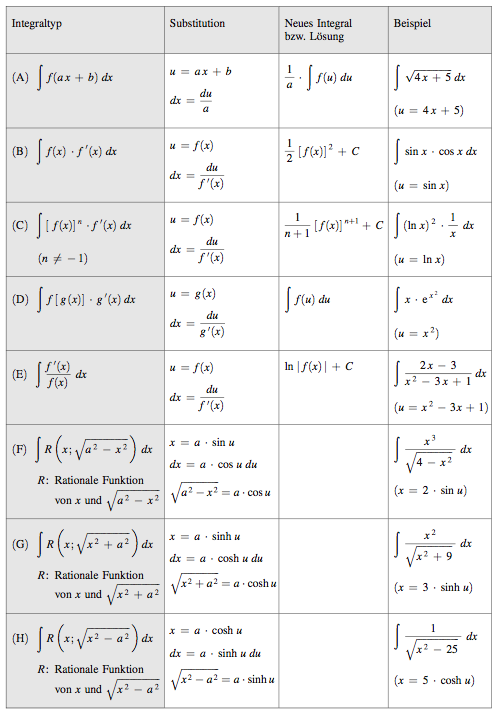
\includegraphics[width=1\linewidth]{img/int1.png}
\end{figure}
\begin{figure}[H]
 	\centering
  	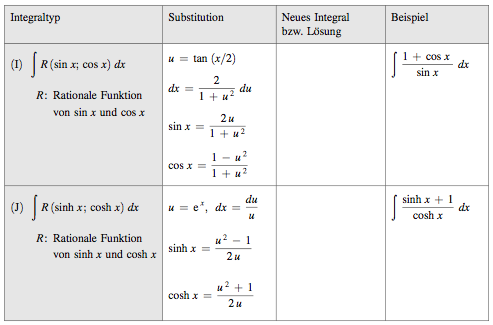
\includegraphics[width=1\linewidth]{img/int2.png}
\end{figure}


\newpage


\begin{warmup}
\subsection{Wertetabellen}

\todo Evt. macht für sin, cos ein Bild mehr sinn.

\begin{tabular}{|c|c|}
\toprule
$x$ & $\sin(x)$\\
$\arcsin(y)$ & $y$\\
\hline
\todo & \todo\\
\bottomrule
\end{tabular}

\begin{tabular}{c|c}
$x$ & $\cos(x)$\\
$\arccos(y)$ & $y$\\
\hline
\todo & \todo
\end{tabular}

\begin{tabular}{c|c}
$x$ & $\tan(x)$\\
$\arctan(y)$ & $y$\\
\hline
\todo & \todo
\end{tabular}

\begin{tabular}{c|c}
$x$ & $\sinh(x)$\\
$\arcsinh(y)$ & $y$\\
\hline
\todo & \todo
\end{tabular}

\begin{tabular}{c|c}
$x$ & $\cosh(x)$\\
$\arccosh(y)$ & $y$\\
\hline
\todo & \todo
\end{tabular}

\begin{tabular}{c|c}
$x$ & $\tanh(x)$\\
$\arctanh(y)$ & $y$\\
\hline
$1$ & $\frac{\pi}{3}$\\
$\sqrt{3}$ & $\frac{\pi}{4}$\\
\todo & \todo
\end{tabular}

\begin{warmup}
\section{Lineare Differentialgleichungen}

In diesem Fall haben wir eine Linearkombination von $y$ und dessen Ableitungen
$y^{(i)}$ und eventuell einen inhomogenen Teil $b$. Aufsteigend sortiert nach dem
Grad der Ableitung kann die DGL in die folgende Form gebracht werden:
\[
a_1(x) y + a_2(x)y' + a_3(x)y^{\prime\prime} + \cdots + a_n(x)y^{(k)} =
\underbrace{b(x)}_{\makebox[0pt]{\text{\tiny inhom. Teil}}}
\]

\todo ich habe gesehen, dass $a_1$ bis $a_n$ nicht nur Konstanten, sondern auch
Funktionsausdrücke $a_i(x)$ sein können: Was ändert sich dann? Was muss man
dann beachten? Kann ich dann noch so vorgehen?

Die Lösungsfunktion $y$ kann nach dem folgenden Schema bestimmt werden, wobei
wir zuerst die Menge der Homogenen Lösasdfasdfasdfasdf:
\todo Genauer beschreiben (evtl. Satz, Superpositionsprinzip)
\[
y = y_h + y_P
\]

\todo Anfangsbedingungen mitreinbringen

\begin{enumerate}[label=(\arabic*)]
  \item \textbf{Finden von $y_h$ durchs Lösen der homogenen DGL:} Dabei lösen
  wir die Differentialgleichung ohne den homogenen Teil. D.h. wir setzen
  $b(x)=0$ und finden die Lösungen für das homogenene Gleichungssystem:
  \[
a_1 y + a_2y' + a_3y^{\prime\prime} + \cdots + a_ny^{(k)} = 0
  \]
  \todo{Kann man hier Gleichungssystem sagen? Oder muss man Gleichung sagen?
  Connection zu Linalg wäre super, dort haben wir das (glaub ich) mit einem GS
  und dem Gaussalg. gelöst.}
  
  Die Lösungsmenge bildet einen Vektorraum der Dimension der Anzahl der
  verschiedenen  der DGL. Sei $k$ die Ordnung der DGL, dann suchen wir $k$
  Basisvektoren, die den Lösungsraum aufspannen.
  
  (Tipp: überprüfe am Ende, ob die Lösungen $\lambda_{i\ldots k}$ vom char.
  Polynom linear unabhängig sind.)
  
  \todo{Ist die Dimension von der Anzahl der verschiedenen vorhandenen
  Ableitungen oder von der Ordnung der DGL abhängig?}
  
  Die Basen für den Vektorraum können beliebig gewählt werden - es wurde aber
  herausgefunden, dass sich folgende Funktion als Basis (bzw. für $y$) besonders
  gut eignet:
  \[
  y:=e^{\lambda x} \quad \text{womit gilt:} \quad y^{(i)} =
  \lambda^{i}e^{\lambda x}
  \]
  
  D.h. wir können die obige DGL folgendermassen schreiben
  \[
  a_1 e^{\lambda x} + a_2\lambda e^{\lambda x} + a_3\lambda^2e^{\lambda x} +
  \cdots + a_n\lambda^{k}e^{\lambda x} = 0
  \]
  wobei wir $e^{\lambda x}$ ausklammern können
  \[
  e^{\lambda x}\underbrace{(a_1 + a_2\lambda  + a_3\lambda^2 + \cdots +
  a_n\lambda^{k})}_{\text{charakteristisches Polynom}} = 0
  \]
  
  Wir sehen, dass nur das charakteristische Polynom eine Nullstelle haben kann
  und suchen jetzt dementsprechend seine Nullstellen.
  
  (Tipp: Das charakteristische Polynom kann direkt dadurch gebildet werden,
  indem man bei der DGL einfach $a_jy^{(i)}$ jeweils mit $a_j\lambda^{i}$
  ersetzt und $b(x)=0$ setzt.)
  
  Um die Nullstellen zu erhalten suchen wir die Nullstellen (Satz von
  Vieta, Binomische Formeln etc.) Eventuell sehen wir die Faktorisierung in
  irreduzible Polynome auch direkt.
  
  \todo Satz von Vieta noch aufschreiben, Bin Formel 3. Grades!
  
  Seien $\lambda_{1\ldots k}$ die entsprechenden Nullstellen, dann setzen wir
  diese in die Gleichung ein.
  
  \todo Woher weiss ich an welcher Stelle ich ein jeweiliges $\lambda_i$
  einsetzen darf?
  
  \todo Ich weiss nicht was die Schritte dazwischen sind um zum folgenden zu
  kommen:
  
  Wir können jetzt anhand der gefundenen Nullstellen $\lambda_{1\ldots k}$ die
  Funktion $y_h$ folgendermassen ermitteln, wobei die Konstanten $c_1$ bis
  $c_k$ frei wählbare skalare Vielfache sind:
  
  \todo $c_1$ bis $c_k$ sind beliebig wählbar richtig? Sie sind sozusagen
  die Skalierungsfaktoren der Basisvektoren, die den Nullraum aufspannen? Wie
  kann es sein, dass es noch eine partikuläre Lösung gibt ausserhalb des
  Nullraumes? Wo gibt es im Definitionsraum noch mehr Dimensionalität?
  \[
  	y_h = c_1\cdot e^{\lambda_1x} + c_2\cdot e^{\lambda_2x} + \cdots + c_k\cdot
  	e^{\lambda_k x}
  \]
  Wollen wir eine \todo (reelle? oder was genau?) Lösung für $y$ erhalten, dann
  ersetzen wir die $e^{\lambda_i x}$-Terme mithilfe der Euler'schen Identität,
   wobei $\lambda_i$ jeweils als $\lambda_i=a_i + b_ii$ geschrieben werden kann:
  \begin{align*}
  e^{\lambda_i x} &=
  e^{(a_i + b_i i)x} = e^{a_ix}\cdot e^{b_ixi}=e^{a_ix}\cdot \cis(b_ix)\\
  &= e^{a_ix} \cdot(\cos(b_ix)+i\sin(b_ix))
  \end{align*}
  
  Somit sieht dann $y_h$ folgendermassen aus
  \begin{align*}
  y_h = &\quad c_1 e^{a_1x} \cdot (\cos(b_1x)+i\sin(b_1x))\\
      &+ c_2 e^{a_2x} \cdot (\cos(b_2x)+i\sin(b_2x))\\
      & \qquad \vdots\\
      &+ c_k e^{a_kx} \cdot (\cos(b_kx)+i\sin(b_kx))\\
  \end{align*}
  
  \todo Schreiben wie wir $y$ in eine Form ohne $i$ bringen mithilfe des
  Satzes der sagt, dass $i$ verschwinden muss. So etwas ähnliches wie die DGL
  hat nur relle Koeffizienten, also muss es auch $y_h$ haben\ldots
  
  Damit haben wir nun $y_h$ endgültig bestimmt.
  
\item \textbf{Finden von $y_P$ durch  \ldots \todo wie genau?}

  $y_P$ wird gefunden, indem wir erraten (Ansatz der rechten Seite, Variation
  der Konstanten), was $y_P$ ungefähr sein könnte.
\end{enumerate}
  
\newpage

\textbf{Ansatz der rechten Seite}

Den inhomogenen Teil $b(x)$ kann man als Störfunktion betrachten, der die
\ldots \todo beeinflusst.

$a,b,c,d\in \R$ \quad $\mu,\nu\in\R$ \quad $n\in \N$

\begin{tabular}{cc}
\toprule
\textbf{Störfunktion} $b(x)$ & \textbf{Ansatz für} $y_p(x)$\\
\midrule
$ae^{\mu x}$ & $be^{\mu x}$
\\
\hline
$\begin{matrix}
a\sin(\nu x)\\
b\cos(\nu x)
\end{matrix}$
& $c\sin(\nu x) + d \cos(\nu x)$
\\
\hline
$\begin{matrix}
ae^{\mu x}\sin(\nu x)\\
be^{\mu x}\cos(\nu x)
\end{matrix}$
&
$e^{\mu x}(c\sin(\nu x) + d\cos(\nu x))$
\\
\hline
$P_n(x)e^{\mu x}$ & $R_n(x)e^{\mu x}$
\\
\hline
$P_n(x)$ & $R_n(x)$
\\
\hline
$\begin{matrix}
P_n(x)e^{\mu x}\sin(\nu x)\\
Q_n(x)e^{\mu x}\cos(\nu x)
\end{matrix}$
&
$e^{\mu x}\left(
R_n(x)\sin(\nu x) +
S_n(x)\cos(\nu x)
\right)$\\
\bottomrule
\end{tabular}

\todo Kann man allgemein sagen was man macht wenn die Störfunktion nur $P_n(x)$
is?

\Bem Liegt eine Linearkombination der Störfunktionen vor, so hat man auch als
Ansatz eine entsprechende Linearkombination zu wählen.

\Bem Falls $\lambda=\mu + i\nu$ eine $m$-fache Nullstelle des charakteristischen
Polynoms (siehe Bestimmung von $y_h$) ist, so muss man den Ansatz für $y_p(x)$
mit dem Faktor $x^m$ multiplizieren. 

\todo Wie war hier genau der Zusammenhang? Es hatte mit Eigenvektoren und
Resonanz zu tun.

\todo Woran scheitert man wenn man den Ansatz falsch gewählt hat? Woran merkt
man dass man gescheitert ist?

Hat man einen Ansatz gewählt, leitet man $y_p(x)$ bis zur höchsten Ordnung $k$
der ursprünglichen DGL ab und setzt dann, die jeweiligen $y^{(i)}_p(x)$ in der
Differentialgleichung für $y^{(i)}$ ein. Die durchs Einsetzen erhaltene
Differentialgleichung fasst man dan schön zusammen, dafür gibt es zwei
Vorgehensweisen:
\begin{itemize}
  \item Nach den unbekannten Variablen: nach den unbekannten Variablen (z.B.
  Koeffizienten der Polynome, oder wie oben auch noch nach $c$, $d$) die durch
   den gewählten Ansatz entstanden
sind.
\item Nach Potenzen von $x$ oder der Form der Störfunktion: so dass man einen
 Koeffizientenvergleich oder ähnliches machen kann.
\end{itemize}

In beiden Fällen erhält man dan eine Gleichung, je nach dem kann man dann
entweder Werte für $x$ einsetzen, oder die Formen und Werte vergleichen (z.B.
Koeffizientenvergleich bei Polynomen). Diese erhaltene Gleichung ist erfüllt für
alle $x$ innerhalb des Definitionsbereichs. Wir dürfen deshalb beliebige
(zulässige) Werte aus dem Definitionsbereich für $x$ einsetzen, und erhalten
jeweils eine wahre Aussage. Wir setzen dabei höchstens so viele verschiedene
Werte für $x$ ein, wie wir unbekannte Variablen haben, so dass wir genau so
viele Gleichungen/Aussagen entstehen, und diese z.B. mit dem Gauss'sche
Eliminationsverfahren gelöst werden können.

\sep

\Bsp (Midterm Aufgabe 3)
\[
\text{DGL:} \qquad y^{\prime\prime\prime}-3y^{\prime\prime}+y'-3y = \frac{x^3}{3}
\]
\textbf{Gewählter Ansatz für $y_p$:} $y_p$ muss ein Polynom 3. Grades sein.

\textbf{Ableitungen von $y_p$:} Wir bilden zuerst alle Ableitungen des
allgemeinen Polynomes 3 Grades, das wir für $y_p$ als Ansatz gewählt haben.
\begin{align*}
y_p   &= ax^2+bx+c\\
y_p'  &= 2ax + b\\
y_p^{\prime\prime} &= 2a\\
y_p^{(3)} &= 0
\end{align*}

\textbf{Einsetzen der Ableitungen:} Wir setzen den Ansatz $y_p$ die erhaltenen
Ableitungen $y_p^{(i)}$ für $y^{(i)}$ in die ursprüngliche DGL ein:
\[
0 -6a + 2ax + b -3ax^2 -3bx -3c = \frac{x^2}{3}
\]

\textbf{Zusammenfassen der nach Potenzen von $x$:} Nun fassen wir die Potenzen
von $x$ zusammen, um einen Koeffizientenvergleich zu machen:
\[
(-3a)\cdot x^2	+ (2a-3b)\cdot x + (b-6a-3c) = \frac{x^3}{3}
\]

\textbf{Bestimmen der Unebkannten durch Koeffizientenvergleich:} Die
vorangehende Form erlaubt uns einfach folgendes Gleichungssystem zu bilden.
\[
\begin{array} {|rcl|} 
-3a &= &\frac{1}{3}\\
2a -3b &= &0\\
b -6a -3c &= &0\\
\end{array}
\]
Daraus ergeben sich für unsere Unbekannten die Lösungen $a=-\frac{1}{9}$,
$b=-\frac{2}{27}$ und $c=\frac{8}{17}$.

Damit kann die partikuläre Lösung der DGL folgendermassen geschrieben werden
\[
y_p = -\frac{1}{9}x^2 -\frac{2}{27}x + \frac{8}{17}.
\]

\sep 

\newpage
 Haben, wir $y_h$
  einmal gefunden, können wir $y_h$ einfach $k$-Mal ableiten, und die
  Ableitungen $y_h^{(i)}$ wie in der ursprünglichen DGL für $y$ einsetzen. Damit
  erhalten wir:
  \[
	a_1(x)y_h + a_2(x)y_h' + a_3(x)y_h^{\prime\prime} + \cdots + a_n(x)y_h^{(k)} =
	\underbrace{b(x)}_{\makebox[0pt]{\text{\tiny inhom. Teil}}}
  \]
\end{warmup}

\newpage

\section{TODOS}

Das gelbe Rechenbuch anschauen - Integration (Regeln, Shortcuts etc.)

-

Ableitungen von Trigonometrischen Funktionen, inkl $\sinh$, $\cosh$ etc.

- 

Trigonometrische Identitäten  (Genauso für sinh, cosh)

-

Wichtigste Werte der Trigonometrischen Funktionen, im speziellen von sinh und
cosh

-

Wichtig: Riemann Summen, Definition von Feinheit und Partition, Beispiel

-

Übersicht von Trigonometrischen Funktionen,
Definitions und Bild/Wertebereich, Graphen, Identitäten, Theoreme.

-

Höhere Binomische Formel

-

Trick, $x^2$ aus der Wurzel ziehen.

-

Ableitungen und Integrale gängiger Funktionen

-

\todo \todo \todo Unbedingt die Plots und die wichtigsten Funktionswerte von
$\cosh$, $\sinh$ und $\tanh$ aufschreiben!!!!!!!

\end{warmup}

\end{multicols*}
\end{document}
